\documentclass[
	a4paper,
	twoside,
	11pt,
	numbers=noenddot, 				% No dot after numbers for chapters, sections, etc.
	cleardoublepage=empty, 			% Left plain page before chapters
	%DIV=15,            			% Adjust this value for more/less text on pages
	BCOR=5mm 						% Binding correction
]{scrbook}

%%%%%%%%%%%%%%%%%%%%%%%%%%%%%%
%%%%%%%%%% Preamble %%%%%%%%%%
%%%%%%%%%%%%%%%%%%%%%%%%%%%%%%

% Kopf- und Fusszeile
\usepackage[automark,headsepline,]{scrpage2} 	% Package scrpage2 erlaubt es die Kopf- und Fußzeile zu gestalten. Optionen sind automark oder manualmark
\pagestyle{scrplain}				% Nur Seitenzahl in Fußzeile. Sonst bleibt Kopf- und Fußzeile leer. Mit "headings" wird Kopf- und Fußzeile eingebunden
\ofoot[]{} 							% Seitenzahl am Rand wird nur gesetzt wenn \pagemark eingefügt wird. Wenn es leer bleibt wird nichts geschrieben
\cfoot[\pagemark]{\pagemark} 		% Seitenzahlen in der Seitenmitte, wenn \pagemark eingefügt. Ansonsten keine Seite

\setlength{\parindent}{0pt} 		% Indent ist set to the given value

% Sprache
\usepackage[english, german]{babel}
\usepackage{verbatim} 				% Text in the env "comment" is interpreted as a comment

% mathematical packages
\usepackage{amsmath}
\usepackage{mathtools}
\usepackage{amssymb}
\usepackage{physics} 				% Usefull package for physical and mathematical formulas. Package-documentation: http://ftp.fau.de/ctan/macros/latex/contrib/physics/physics.pdf
%\usepackage{bbold}					% to write the unit element like lettes with \mathbb
\usepackage{dsfont}					% to write the unit element with \mathds, see: http://milde.users.sourceforge.net/LUCR/Math/mathpackages/dsfont-symbols.pdf

% package for including graphics
\usepackage{graphicx}
\usepackage{subfigure} 				% Package for setting two graphics side by side
\usepackage{epstopdf} 				% Convert eps-files to pdf-files
\graphicspath{{figures/}} 			% Path to all figures used in this document

\usepackage{bm}						% Make the argument bold
\usepackage{xcolor}					% Package for changing he color of letters, numbers and other things 
\usepackage{float}					% Improve interface of floating objects

\usepackage{enumitem} 				% change the level in enumerate-envirement

\usepackage[draft]{todonotes}   	% draft: notes showed, disable: not showed

% feynman and wick stuff
\usepackage{simplewick}				% drawing wick contractions above or below a set of operators. See http://ftp.riken.jp/tex-archive/macros/latex/contrib/simplewick/simplewick.pdf

% bibiography package and stylesetting
\usepackage[
	backend = biber, 
	bibencoding = utf8,
	style = alphabetic, 
	sorting = none, 
	autocite = plain, 
	language = autobib,
]{biblatex} 
\addbibresource{bibliography/masterthesis.bib}
\usepackage{csquotes}
\usepackage[colorlinks=true, linkcolor=black, citecolor=black, urlcolor=blue]{hyperref}
%\usepackage{hyperref}
%\usepackage[figure,table]{hypcap}               % to correct a problem with hyperref
%\hypersetup{
%	pdftitle = {},
%	pdfsubject = {},
%	pdfauthor = {},
%	pdfkeywords = {},
%	pdfcreator = {},
%	pdfproducer = {LaTeX with hyperref},
%	colorlinks = true,
%	linkcolor = blue,
%	anchorcolor = blue,
%	citecolor = blue,
%	filecolor = red,
%	menucolor = red,
%	pagecolor = red,
%	urlcolor  = blue,
%	breaklinks = true,
%	pdfstartview = FitV,
%	pdfhighlight = /I,
%	pdfpagelayout = OneColumn,
%	hypertexnames=true
%}


%%%%%%%%%%%%%%%%%%%%%%%%%%%%%%%%%%%%%%%%%
%%%%%%%%%% self-defined macros %%%%%%%%%%
%%%%%%%%%%%%%%%%%%%%%%%%%%%%%%%%%%%%%%%%%

\newcommand{\mt}[1]{\mathrm{#1}} %%% text in math-mode get normal like you aren't in math-mode

%%% braket notation in the hilbertspace of operators (Liouville space) %%%

\newcommand{\oket}[1]{\big|{#1}\big)} % ket in operator space with automatic sizing
\newcommand{\toket}[1]{|\mt{#1})} % ket in operator space for writing inside normal text

\newcommand{\obra}[1]{\big({#1}\big|} % bra in operator space with automatic sizing
\newcommand{\tobra}[1]{(\mt{#1}|} % bra in operator space for writing inside normal text

\newcommand{\obraket}[2]{\big({#1}\big|{#2}\big)} % braket in operator space with automatic sizing
\newcommand{\tobraket}[2]{({#1}|{#2})} % braket in operator space for writing inside normal text

\newcommand{\odyad}[2]{\oket{#1}\obra{#2}} % dyad in operator space with autometic sizing
\newcommand{\tdyad}[2]{\toket{#1}\tobra{#2}} % dyad in operator space for writing inside normal text

\newcommand{\ie}{i.\,e.}

%\newcommand{\ev}[1]{\left\langle{#1}\right\rangle} 											% expactation value
%\newcommand{\erwartungswert}[3]{\left\langle {#1}\right|{#2}\left|{#3}\right\rangle} 		% ausführlicher erwartungswert mit zuständen
%\newcommand{\kom}[2]{\Big[{#1},{#2}\Big]} 													% commutator
%\newcommand{\antikom}[2]{\Big\{{#1},{#2}\Big\}} 											% anticommutator
%\newcommand{\integral}[4]{\int\limits_{{#1}}^{{#2}}{#3}\ {#4}} 								% integral: #1->lower limit; #2->upper limit; #3->differential operator; #4->integrand
%\newcommand{\scalarproduct}[2]{\left({#1}|{#2}\right)} 										% scalar product super operator
%\newcommand{\opnorm}[1]{\left({#1}|{#1}\right)} 											% norm super operator
%\newcommand{\evso}[3]{\left({#1}\right|{#2}\left|{#3}\right)} 								% expactation value super operator
%\newcommand{\projectionoperator}[2]{\frac{\left|{#1}\right)\left({#2}\right|}{\opnorm{#2}}} % projectionoperator super operator
%\newcommand{\opket}[1]{\left|{#1}\right)} 													% operator ket
%\newcommand{\opbra}[1]{\left({#1}\right|} 													% operator bra
%\newcommand{\trace}[1]{\mathrm{Tr}\left\{{#1}\right\}} 										% trace
\newcommand{\green}[2]{\big\langle\big\langle{#1};{#2}\big\rangle\big\rangle} 				% Definition of Green-function with angle brackets
%\newcommand{\totalDif}[1]{\frac{\mathrm{d}}{\mathrm{d}{#1}}} 								% totale differentiation
%\newcommand{\partialDif}[1]{\frac{\partial}{\partial{#1}}} 									% partielle differentiation
%\newcommand{\longkom}[2]{\Big[{#1},\vphantom{\Big]}\notag\\\vphantom{\Big[}&{#2}\Big]} 		% commutator with linebreak between #1 und #2
%\newcommand{\longev}[2]{\Big\langle{#1}\\ &{#2}\Big\rangle}									% expectation value with linebreak between #1 and #2

% Vectors and matricies
%\newcommand{\bvec}[1]{\textbf{#1}} 															% vector bold letter
\newcommand{\oneTwoVec}[2]{\begin{pmatrix}#1 & #2\end{pmatrix}} 							% two componand row vector
\newcommand{\twoOneVec}[2]{\begin{pmatrix}#1\\#2\end{pmatrix}} 								% two componand column vector
\newcommand{\twoTwoMatrix}[4]{\begin{pmatrix}#1 & #2\\#3 & #4\end{pmatrix}} 				% 2x2 matrix

% Fourier transformation
%\newcommand{\fouriertrafo}[4]{\int \frac{\mathrm{d}^{#4}{#3}}{(2\pi)^{#4}}\, {#1}({#3},\tau) e^{#2}} % Fouriertrafo into momentum space (#1: function; #2: argument of e; #3: momentum letter; #4: dimension)

% definition of mathematical functions
\DeclareMathOperator{\sign}{sign}
%\DeclareMathOperator{\Real}{Re}
%\DeclareMathOperator{\Imag}{Im}

%%%%%%%%%%%%%%%%%%%%%%%%%%%%
%%%%%%%%%% Layout %%%%%%%%%%
%%%%%%%%%%%%%%%%%%%%%%%%%%%%








%%%%%%%%%%%%%%%%%%%%%%%%%%%%%%%%%%%%%%%%%%%%%%%
%%%%%%%%%% Beginning of the document %%%%%%%%%%
%%%%%%%%%%%%%%%%%%%%%%%%%%%%%%%%%%%%%%%%%%%%%%%

\begin{document}

\pagestyle{empty}					% no pagestyle -> no heading, no numbering
\selectlanguage{german}				% document language set to german

%%% Your personal titlepage in german
%%% Can be used for diplomathesises
%%%
%%% adjust all the red colored text and remove the color tags

\begin{titlepage}
  \rmfamily
  \begin{center}
    { \Large
      \hrule
      \vspace{1em}
      \begin{center}

        \begin{minipage}[hbt]{4cm}
          \centering
          \includegraphics[draft=false, width=3cm]{logos/KITlogo_transparent.eps}
        \end{minipage}
        \begin{minipage}[hbt]{11cm}
		\vspace{1ex}          
          Fakult"at f"ur Physik

          Institut f"ur Theorie der Kondensierten Materie
        \end{minipage}
      \end{center}
      \vspace{1em}
      \hrule 
    } 
    \vspace*{\stretch{11}}
    { 
      \LARGE\bfseries
      Quantum Transport in Spin Density Systems with the Memory-Matrix-Formalism\\
      %Quantentransport in Spindichtesystemen mit dem Memory-Matrix-Formalismus\\       
    }
    \vspace*{\stretch{14}}
    {
      %\includegraphics[width=10cm]{Titlepage/cover}\\
    }
    \vspace*{\stretch{8}}
    { \Large
      Masterthesis \\
      \vspace*{\stretch{0.5}}
      von \\
      \vspace*{\stretch{0.5}}
      Martin Lietz\\
    }
    \vspace*{\stretch{2}}
    { \large 
      27.\,Mai\,2017 bis 27.\,Mai\,2018\\
    }
    \vspace*{\stretch{5}}
    { \large
      \begin{tabular}{r@{\hspace{2em}}l}
        Referent:     & Prof.\,Dr.\,J"org Schmalian\\
        Korreferent:  & Prof.\,Dr.\,Alexander Shnirman
      \end{tabular}
    }
  \end{center}
  \vspace*{\stretch{1}}
\end{titlepage}
\cleardoublepage
		% titlepage in german
%\input{misc/titlepage_english}		% titlepage in english

\frontmatter						% activate roman numbering
\pagestyle{plain}

\cleardoublepage
\input{misc/assertion_german}		% assertion in german

\selectlanguage{english}			% document language set to english
\cleardoublepage
%
%
\chapter*{Acknowledgment}
%
%
I would firstly like to thank my advisior Prof.\,Dr.\,J\"org Schmalian for offeringme the opportunity to write my master thesis at his institute.
The door to Prof.\,Schmalian's office was always open whenever I ran into trouble at my research.
All the fruitful discussions have influenced my point of view to think about phyisics.
Furthermore, I would to thank Prof.\,Schmalian for the great support apart from reasearch topics.

\vspace{1em}
\noindent I would also like to acknowledge Prof.\,Dr.\,Alexander Shnirman as the second reader of this thesis.

\vspace{1em}
\noindent I would also like to thank all the people at the institute of condensed matter theory (TKM) at the KIT for the hearty welcome, great support and the nice time.

\vspace{1em}
\noindent Finally, I must express my very profound gratitude to may parents, my sister and my love Vanessa for providing me with unfailing support and continous encouragement throughout my years  of study and through the process of researching and writing this thesis.
This accomplishment would not have been possible without them. 

\vspace{2em}
\noindent Thank you.

\vspace{1em}
\noindent Martin Lietz		% help from colleagues and friends

\cleardoublepage
\tableofcontents					% table of contents

\pagestyle{scrheadings}				% activate heading and numbering
\mainmatter							% activate	arabic numbering

% includeing chapters
\begingroup
\allowdisplaybreaks
\cleardoublepage
%
%
\chapter{Introduction}
\label{ch:introduction}
%
%
The electrical conductivity or resistance is a fundamental characteristic and an accessable observable of metals.
The response of electrons as a consequence of an external applied electrical field is measured by the conductivity and its magnitude is finite due to internal processes.
A first physical explanation describing this circumstances was published by Drude \cite{Drude} in the year 1900.
He supposed the electrons to be free particles moving around in the metal.
As a consequence of scattering, the electrons are assumed to possess a finite relaxation time $\tau$.
The passing time between to scattering events is denoted by this characteristical variable.
At low temperatures, the electrical conductivity is determined by scattering between electrons and impurities.
The fact, that non-conservation of momentum due to relaxation and a finite electrical conductivity are directly associated, is demonstrated by Drude's theory.
The results of this phenomenological theory are exactly confirmed by using the technique of quantum field theory without considering quantum correction to describe the electrons \cite{Bruus&Flensberg}.
Landau's Fermi liquid theory is the well proven quantum mechanical describtion for metals.
%Metals are well described by Landau's Fermi liquid theory in quantum mechanics.
A quadratic temperature dependence of the resistance $\rho(T) = \rho_{0} + A \cdot T^{2}$, where $\rho_{0}$ is the saturation resistance from impurity scattering at low temperatures \cite{Bader,Pal} is generated by taking into account electron-electron interaction as well as umklapp scattering.
This temperature dependence is modified by quantum mechanical corrections, like weak localization \cite{Altshuler} and the Kondo effect \cite{Kondo}.
A logarithmical increase of the resistance at small temperatures $T < T_{\mt{K}} \approx 1-10\,\mt{K}$ \cite{Kouwenhoven&Glazman} due to electron scattering with localizied magnetic impurities is described by the Kondo effect.
These modifications in the temperature dependence of the resistance are delineated well by Landau's Fermi liquid theory considering quantum corrections.
A non-Fermi liquid behaviour, that is characterizied in a linear temperature dependence of the resistance $\rho(T) = \rho_{0} + A \cdot T$ \cite{Loehneysen}, is  discovered in alloys, like $\mt{CeCu}_{5.9}\mt{Au}_{0.1}$ and $\mt{CeCu}_{5.8}\mt{Ag}_{0.2}$.

The origin of this strange and unexpected behaviour is a quantum phase transition of second order.
In comparison to normal phase transitions, which result from thermal fluctuations, quantum phase transitions are generated by quantum fluctuations.
The phase diagram of such a quantum phase transition is characterizied by a quantum critical point at temperature $T=0$ and a critical tuning parameter $\mt{g}=\mt{g}_{\mt{c}}$.
This tuning parameter has to be a physical parameter, like external pressure, an external applied field or the chemical composition.
It is not possible to reach the absolute zero, but this does not mean that the existence of the quantum critical point and the corresponding quantum fluctuations can not be measured.
At temperatures of several mK, the magnitude of quantum fluctuations is comparable to thermal fluctuations.
The interplay between fermionic Landau quasiparticles and bosonic fluctuations constitute the physical origin of these quantum fluctuations.
The behaviour of quasiparticles becomes critical and as a conseqence of that they acting back to the bosonic fluctuations \cite{Abrahams&Schmalian&Woelfle}
A strong coupling carried by bosonic fluctuations emerges between fermions.

An antiferromagnetic quantum phase transition is generated in the heavy-fermion compounds $\mt{CeCu}_{5.9}\mt{Au}_{0.1}$ and $\mt{CeCu}_{5.8}\mt{Ag}_{0.2}$.
A microscopical description is presented by Abanov et.\,al. \cite{Abanov&Chubukov&Schmalian} in the two dimensional spin-fermion-model containing fermionic quasiparticles and spin density waves.
Spin fluctuations are created at the vicinity of the quantum critical point as a result of permanent particle-holes excitations.
The propagation of these fluctuations is described by the dynamical magnetic susceptibility.
A sharp peak at a large momentum vector $\vb{Q}$ is visable in its spectrum.
As a consequence, a strong interaction between fermions on the Fermi surface seperated by this vector is caused by spin fluctuations.
These certain points on the Fermi surface are called hot spots.

Patel and Sachdev \cite{Patel&Sachdev} make use of the spin-fermion-model modified with an \linebreak anisotropic parapolical fermionic dispersion to discribe the linear temperature dependence of the resistance.
Their computation is based on the memory-matrix-formalism that was firstly pupblished by Mori \cite{Mori} in the year 1965.
The memory-matrix-formalism is grounded on two fundamental ideas: 
1) The ensemble density is seperated into two parts.
One of them contains all the \emph{relevant} amounts determining the mean value of specific observables, while the remaining amounts are denoted as \emph{irrelevant} \cite{Zwanzig}.
2) The memory function $\mt{M}(z)$ decays exponentially in time, $\mt{M}(z) \sim \exp(-\flatfrac{t}{\tau_{\mt{c}}})$, where $\tau_{\mt{c}}$ is the correlation time.
The time evolution of an autocorrelation function is determined by the memory function containing the history of the correlation function \cite{Berne&Boob&Rice}.
In general, the time evolution is described by the memory-matrix-formalism for small time scales.
The memory function decays very slow to zero in the case of conserved quantities.
The time evolution is consequently detemined for large times or small frequencies.
This circumstance is used by Patel and Sachdev to compute the static electrical conductivity in the spin-fermion-model perturbed by a random potential term for fermions and a random-mass term for the bosonic field \cite{Patel&Sachdev}.
A linear resistance is shown using this treatment in both cases.

Beside these two effect, umklapp scattering has also to be taken into account as a possible origin for the linear temperature behaviour of the resistance.
The calculation of the static electrical conductivity similar to the treatment of Patel and Sachdev is presented in this thesis.

\paragraph{Outline of this thesis}$\:$\vspace{3.5ex}

In chapter \ref{ch:infinite conductivity} it is shown that the static electrical conductivity is generally infinite in a system that conserve momentum and do not conserve current. 
A short review over the memory-matrix-formalism is given.
Two fundamental conditions are therefore required: 
1) The Hamiltonian is invariant with respect to time reversal symmetry.
2) The corresponing variables are momentum and current.
Both quantities are assumed to have the same sign under time reversal symmetry.

The spin-fermion-model is introduced in chapter \ref{ch:spin fermion model}.
It is used in our later calculation in chapter \ref{ch:calculation}.
An overview over the principles of quantum phase transitions and appearing characteristic parameters is given.
The temperature dependence of the correlation length is discussed.
The spin-fermion-model is discussed in detail: the propagator of spin fluctuations and the appearance of damping are explained.
Furthermore, the basic concepts of the hot spots theory is presented.
The conservation of momentum and current is illustarted for the spin-fermion model in two cases:
1) unperturbed and 
2) perturbed by umklapp scattering.

In chapter \ref{ch:calculation}, the calculation of the static electrical conductivity is presentet for the spin-fermion-model pertubated by umklapp scattering.
This is divided into two parts.
The temperature dependence of the susceptibility $\chi_{\mt{JP}}$ is determined and the Green function $\mathcal{G}_{\dot{\mt{P}}\dot{\mt{P}}}(\vb{k},z)$ is calculated.
In both cases, the diagrammatic pertubation theory is utilizied, whereas in the latter the integral is analyzied approximately.

Chapter \ref{ch:memory matrix formalism} gives a detailed overview over the memory-matrix-formalism.
The mathematical framework is defined by introducing the Liouville space.
Afterwards, an explicite expression of the autocorrelation function is derivated depending on the memory function $\mt{M}(z)$.
The Evidence that dissipative effect in $\mt{M}(z)$ disappear is proved under the conditions: 
1) The Hamiltonian is invariant with respect to time reversal symmetry.
2) The corresponding operators are assumed to have the same sign under time reversal symmetry.
Finally, the expression to calculate the static conductivity is derived.

\paragraph{Notation}$\:$\vspace{3.5ex}

In this masterthesis, we chose units where $\hbar = k_{\mt{B}} = 1$ and with that $\beta = T^{-1}$.
The intergation over the first two dimensional Brillouin zone and the sums over spatial directions or the fermion species a and b is abbreviated with the symbols:
%
\begin{align}
	&\int_{\vb{k}} := \int\limits_{\mt{BZ}} \frac{\dd[2]{\vb{k}}}{(2\pi)^{2}}
	\\
	&\sum\limits_{\mu} := \sum\limits_{\mu = 1}^{3} \qq{equally} \lambda
	\\
	&\sum\limits_{\alpha} := \sum\limits_{\alpha = a,b} \qq{equally} \beta \qq{and} \gamma
	\\
	&\sum\limits_{\alpha\neq\beta} := \sum\limits_{\substack{\alpha = a,b \\ \alpha\neq\beta}} \sum_{\beta = a,b}
\end{align}
%
Furthermore, these integrals are usefull in our calculation \cite{Bronstein}:
%
\begin{align}
	\int \dd{x} \frac{1}{(z^{2} + 1)^{2}} = \frac{1}{2}\Big[\frac{z}{z^2 + 1} + \tan[-1](z)\Big]
	\label{eq:integral1}
	\\
	\int\limits_{0}^{\infty} \dd{x} \frac{x}{a^{2} + x^{2}} \cdot \frac{x}{y^{2} + x^{2}} = \frac{\pi}{2} \frac{1}{a + |y|}
	\label{eq:integral2}
\end{align}
%





































%
\cleardoublepage
%
%
%
\chapter{Infinite Static Conductivity in Translation Invariant Systems}
\label{ch:infinite conductivity}
%
%
%
Ever since Drude published his theory about the electrical conductivity in metals \cite{Drude} at the beginning of the last century, it is well known that non-conversion of electron momentum in a system is required for finite electrical conductivity.
In Drude's model, the electrons possess a mean scattering time $\tau_{\mt{el}}$ representing the mean time between two scattering events of an electron and a lattice atom.
At each scattering event, the electrons transfer momentum to the lattice atoms, which is the reason electron momentum is not a conserved quantity.
In the case of conserved momentum, if an electrical field is exemplary applied, it accelerates electrons up to an infinite velocity, causing infinite conductivity.

In the following section, a momentum conserving system is considered and the electrical conductivity is computed using the memory-matrix-formalism, where an infinite conductivity is expected.
Beforehand, a short overview over the memory-matrix-formalism is given, followed by detailed and explicite deviations in chapter \ref{ch:memory matrix formalism}.
%
%
\section{An Overview over the Memory-Matrix-Formalsim}
\label{sec:overview MMF}
%
%
Let us assume a physical dynamical variable $\mt{A}(t)$ in an arbitrary system and an arbitrary pertubation too	.
Our interest is now the time evolution of $\mt{A}(t)$ depending on the pertubation.
Completely general, a physical dynamical variable can be splitted into two parts, a secular one and a non-secular one, which is shown in \cite{Mori}.
The latter represent processes like fluctuations or initial transient processes, which have in common a short lifetime comparing to the secular processes.
The dynamic and time evolution of $\mt{A}(t)$ is therefore dominated by secular processes.

This seperation enables a simple but clever geometrical interpretation, where dynamical variables are considered to be vectors in a vector space.
The direction of the variable $\mt{A}(t)$ is denoted as the A-axis, considering a unpertubated system in equilibrium.
Switching on a pertubation, the system is moved out of the equilibrium state and as a consequence the direction of $\mt{A}(t)$ is modified.
The projection of $\mt{A}(t)$ onto the A-axis is identified with the secular part, while the non-secular part is the part perpendicular to the projection 

First of all, the mathematical framework for this vector space has to be established.
In quantum mechanics, the Liouville space, also called as operator space, is the respective vector space of the memory-matrix-formalism.
As indicated by the name \emph{operator space}, the vectors of the Liouville space are operators, all of which being Hermitian.
The basis of the Liouville space is signified as $\{\toket{\mt{A}_{i}}\}$, where $i = 1,2,3,\dots,n$, and the corresponding dual space basis is denoted as $\{\tobra{\mt{A}_{i}}\}$.
To complete the definition of any vector space, a scalar product is required.
The following one is chosen:
%
\begin{align}
	\obraket{\mt{A}_{i}(t)}{\mt{A}_{j}(t')} = \frac{1}{\beta} \int\limits_{0}^{\beta} \dd{\lambda} \expval{\mt{A}_{i}^{\dag}(t) \mt{A}_{j}(t'+i\lambda)}.
	\label{eq:scalar product Liouville space}
\end{align}
%
The normal time evolution $\mt{A}_{i}(t) = e^{i\mt{H}t/\hbar} \mt{A}_{i}(0) e^{-i\mt{H}t/\hbar}$ of an operator should be valid so that $\mt{A}_{i}(i\lambda) = e^{-\lambda\mt{H}} \mt{A}_{i}(0) e^{\lambda\mt{H}}$ can be used.
If secular processes are neglected, the choice of the scalar product is determined under the aspect that as a consequence the time evolution of $\mt{A}(t)$ given the most probably path, see \cite{Mori}.
In quantum mechanics, the dynamic of an operator is ususally described by the Heisenberg equation of motion, which is transformed using the dyad product into the Liouville space
%
\begin{align}
	\oket{\dot{\mt{A}}_{i}(t)} = \frac{i}{\hbar} \oket{\comm{\mt{H}}{\mt{A}_{i}(t)}} = i \mt{L} \oket{\mt{A}_{i}(t)}.
	\label{eq:HEM in LS}
\end{align}
%
Here the Hermitian Liouville operator, ${\mt{L} = \hbar^{-1} \comm{\mt{H}}{\mt{\bullet}}}$, is introduced, which is defined by his action onto an arbitrary operator.
The formal solution of this equation is given by $\toket{\mt{A}_{i}(t)} = \exp(it\mt{L}) \cdot \toket{\mt{A}_{i}(0)}$, where the time evolution of an operator is therefore given by the Liouville operator.
For our approach a further operator is required in the Liouville space, namely the projection operator.
A set of arbitrary operators $\{\mt{C}_{i}\}$ is therefore defined.
The choice of them is different for each observed problem and unimportant at the moment.
The definition of the projection operator in Liouville space follows directly from the projection operator defined in the commonly used Hilbert space in quantum mechanics.
%
\begin{align}
	\mt{P} = \sum\limits_{i,j} \frac{\oket{\mt{C}_{i}(0)} \obra{\mt{C}_{j}(0)}}{\obraket{\mt{C}_{i}(0)}{\mt{C}_{j}(0)}} 
	\label{eq:projection operator}
\end{align}
%
The projection operator acting on some vector in Liouville space yields the projection onto the subspace spanned by the operator $\mt{C}_{i}$.
Thus, the operator $\mt{Q} = 1 - \mt{P}$ yields the corresponding part projected out of the subspace.
Furthermore, the projection operator is Hermitian and fullfills the two properties $\mt{P}^{2} = \mt{P}$ and $\mt{PQ} = \mt{QP} = 0$.
This completes the required mathematical basis of the memory-matrix formalism.

Correlation functions are the natural approach to describe the reaction of a dynamic variable on a pertubation.
In quantum mechanics, the correlation function is defined in Kubo's linear response theory as an integral over an expectation value of two operators, one of them being the investigated operator, and the other one being the coupling operator from the pertubation Hamiltonian.
In the Liouville space, the correlation function is defined as
%
\begin{align}
	\mathcal{C}_{ij}(t) := \obraket{\mt{A}_{i}(t)}{\mt{A}_{j}(0)} = \frac{1}{\beta} \int\limits_{0}^{\beta} \dd{\lambda} \expval{\mt{A}_{i}^{\dag}(t) \mt{A}_{j}(i\lambda\hbar)},
	\label{eq:correlation function in LS}
\end{align}
%
using the definition of the scalar product \eqref{eq:scalar product Liouville space}  in the second step.
Expressing the time evolution of $\mt{A}_{i}(t)$ with the Liouville operator, using the Laplace transformation and a few conversions yields an algebraic matrix equation of the correlation function, which has the form
%
\begin{align}
	\sum\limits_{l} \Big[\omega \delta_{il} - \Omega_{il} + i \Sigma_{il}(\omega)\Big] \mathcal{C}_{lj}(\omega) = \frac{i}{\beta} \chi_{ij}(0),
	\label{eq:algebraic equation correlation function}
\end{align}
%
where the abbreviations 
%
\begin{align}
	\Omega_{il} := i \beta \sum\limits_{k} \obraket{\dot{\mt{A}}_{i}}{\mt{C}_{k}} \chi_{kl}^{-1}(0)
	\qq{and}
	\Sigma_{il}(\omega) := i \beta \sum\limits_{k} \obra{\dot{\mt{A}}_{i}} \mt{Q} \frac{1}{\omega - \mt{QLQ}} \mt{Q} \oket{\dot{\mt{C}}_{k}} \chi_{kl}^{-1}(0)
	\label{eq:Omega&Sigma}
\end{align}
%
are introduced.
Both sums over $l$ and $k$ run over the set of operators, defined by the projection operator.
Similiarly, the indices $i$ and $j$ have to be chosen from this set of operators so that \eqref{eq:algebraic equation correlation function} yields $n^{2}$ equations, if $n$ is the number of operators in the set.
Both abbreviations can be combined to a function $M_{il}(\omega) := \Sigma_{il}(\omega) +i \Omega_{il}$, called the memory function.
In this function, $\Sigma_{il}(\omega)$ takes the role of the quantum mechanical self energy, while $\Omega_{il}$ represents dissipative effects.
$\Omega_{il}$ vanishes under to condictions.
The model Hamiltonian has to be invariant under time reversal symmetry.
Furthermore, both operators, $\mt{A}_{i}$ and $\mt{C}_{k}$, have to be the same sign with respect to time reversal symmetry.
This assertion is proven in great detail in \ref{subsec: time reversal symmetry}.
In folloes that the memory function is solely determined by $\Sigma_{il}(\omega)$.

The structur of $\Sigma_{il}(\omega)$ resembles the one of the Laplace transformed correlation function, comparing equation \eqref{eq:correlation function frequency space}, with two differences.
The expectation value is performed with respect to the operators like $\mt{Q}\toket{\dot{\mt{A}}_{i}}$ instead of $\toket{\mt{A}_{i}}$, while only the reduced Liouville operator QLQ is considered.
The latter projects at the part of the full Liouville operator, which causes the intrinsic fluctuations of the operator $\mt{A}$.
In other words, the operator QLQ describes the internal dynamics of all other degrees of freedom of the system, called the \emph{bath}, excluded A.
The coupling to the bath is characterizied by the vector $\mt{Q}\toket{\dot{\mt{A}}_{i}}$ and is clearly changing the dynamic behaviour of A.
%
%
\section{Electrical Conductivity in a Momentum Conserving System}
\label{sec:conductivity conserved momentum}
%
%
%
\begin{figure}[t]
	\centering
	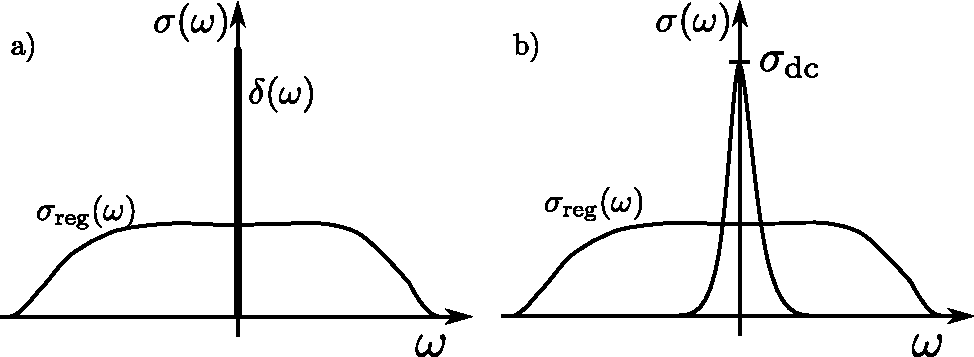
\includegraphics[width=0.9\textwidth]{conductivity.pdf}
	%\subfigure[infinite conductivity considering unbroken translation symmetry]{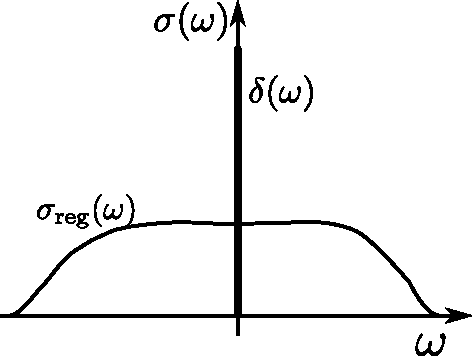
\includegraphics[width=0.45\textwidth]{conductivity_delta_peak.pdf}}
	%\subfigure[finite conductivity considering broken translation symmetry]{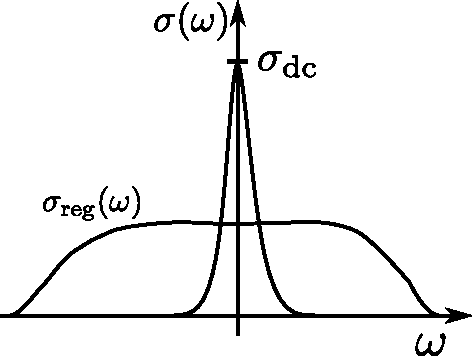
\includegraphics[width=0.45\textwidth]{conductivity_drude_peak.pdf}}
	\caption{
Figure a) and b) shown the static electrical conductivity in a un-pertubated and pertubated system, respectively.
In a system with unbroken translation symmetry, the relaxation of momentum is impossible to other degrees of freedom. 
As a consequence, the static conductivity is infinite. This is illustrated in a).
Switching on a pertubation as umklapp scattering, the translation symmetry is broken.
The static conductivity becomes finite due to the relaxation of momentum to other degrees of freedom.
In both figures, the regular conductivity, caused by fluctuation e.\,g., is denoted as $\sigma_{\mt{dc}}$.
	}
	\label{fig:conductivity broken and unbroken translation symmetry}
\end{figure}
%
In the following section, the electrical conductivity is computed for a system, where momentum is conserved, using the memory-matrix-formalism.
An infinite conductivity is expected due to the fact that electrons do not transfer any momentum to other degrees of freedom.
Besides conserving momentum, the observed system has to satisfy some additional requirements.
Firstly, the current has to be an unconserved quantitiy.
Furthermore, the scalar product $\tobraket{\mt{J}}{\mt{P}}$ of current and momentum has to be non-zero.
In other words, both quantities possess a finite overlap.
These two quantities should also generate the subspace into the projection operator projects.
The sum in \eqref{eq:projection operator} summerizes over all operators $\mt{C}_{i}$, where the choice has now to be done with respect to the electrical conductivity.
As electrical conductivity is determined by momentum and current, these are chosen as operators.
The last requirement is for the Hamiltonian to be invariant under time reversal symmetry, which is our last requirement.

Nevertheless, one remark has to be made for computing the conductivity.
Due to the fact that the Hamiltonian is invariant under time reversal symmetry and the subspace is generated by J and P, which have same signature under time reversal symmetry, no dissipative effects exist.
The quantity $\Omega$, defined in \eqref{eq:Omega&Sigma}, is therefore zero.

In the strictly general sense, the electrical conductivity is given by the current-current correlation function $\mathcal{C}_{\mt{JJ}}(\omega)$ (see \cite{Chycholl2}).
The static case is obtained by taking the small frequency limit, $\omega \to 0$, of the conductivity.
%
\begin{align}
	\sigma_{\mt{dc}} = \lim\limits_{\omega \to 0} \sigma(\omega) = \lim\limits_{\omega \to 0}\, \beta\,\mathcal{C}_{\mt{JJ}}(\omega)
	\label{eq:general static condictivity}
\end{align}
%
The current-current correlation function is given by equation \eqref{eq:algebraic equation correlation function}, which is in the case of the J-P subspace a $2\times2$ matrix equation.
The quantity $\Sigma$ is simplified by two aspects.
Firstly, the momentum is conserved, which means the time derivative of P is zero and therefore all expectation values are trivially zero where $\dot{\mt{P}}$ is a taken vector.
The remaining expectation values of $\Sigma$ contains only the current J, but these ones are vanishing as well.
The operator QLQ describes the intrinsic fluctuation of $\toket{\mt{J}}$, which are assumed to be zero.
Furthermore, the operator Q acting on $\toket{\mt{J}}$ yields the coupling to these intrinsic fluctuation and, leading to $\mt{Q}\toket{\mt{J}} = 0$.
The obtained matrix equation has a very simple form and the current-current correlation function can be directly read out as
%
\begin{align}
	\mathcal{C}_{\mt{JJ}}(z) = \frac{i}{\omega} \beta^{-1} \chi_{\mt{JJ}}(\omega=0) = \frac{i}{\omega} \mathcal{C}_{\mt{JJ}}(t=0),
	\label{eq:correlation function unpertubated system}
\end{align}
%
where relation \eqref{eq:relation between C, Phi and chi} is being used.
The correlation function at time $t = 0$ is given by the scalar product $\tobraket{\mt{J}(0)}{\mt{J}(0)}$ (see \eqref{eq:correlation function in LS}).
Due to the fact that current and momentum are two closely connected quantities, this is also valid for their correlation functions
For this reason, the current-current correlation function is expresed with respect to the momentum-momentum correlation function.

The vector operator $\toket{\mt{J}(0)}$ is seperated into two pieces, one parallel and one perpendicular part, which are labeled as $\oket{\mt{J}_{\mid\mid}}$ and $\oket{\mt{J}_{\bot}}$, respectivily.
As discussed above, every variable generally consists of a secular and non-secular part, which does not mean that both parts need to exist in the observing model.
The non-secular part is represented by the perpendicular component of $\toket{J}$.
In the experiement, these processes are obseved as a constant slowly fluctuating background, known as noise.
The secular part is represented by the parallel component of $\toket{J}$, which is responsible for the electrical condictivity and is visable as a peak in the measurement, depicted in figure \ref{fig:conductivity broken and unbroken translation symmetry}.

Drude's theory of conductivity yields a direct proportionality between J and P (see for example \cite{Gross&Marx}).
Since momentum is conserved and current is unconserved, in the investigated system this proportionality can't be valid.
Nevertheless, both quantities possess a finite overlap, which means that a part of the current is conserved and therefore parallel to the momentum.
This part is the parallel component of J and given by the projection von $\toket{\mt{J}}$ onto $\toket{\mt{P}}$.
%
\begin{align}
	\oket{\mt{J}_{\mid\mid}} = \mathcal{P}\oket{\mt{J}} = \frac{\odyad{\mt{P}}{\mt{P}}}{\obraket{\mt{P}}{\mt{P}}} \oket{\mt{J}} = \frac{\chi_{\mt{PJ}}}{\chi_{\mt{PP}}} \oket{\mt{P}}
	\label{eq:parallel current as projection}
\end{align}
%
Seperating both current operator in $\tobraket{\mt{J}(0)}{\mt{J}(0)}$ yields four new correlation functions, where the mixed ones are zero, since $\oket{\mt{J}_{\mid\mid}}$ and $\oket{\mt{J}_{\bot}}$ are perpendicular to each other by construction.
For the operators in the parallel correlation function, $\tobraket{\mt{J}_{\mid\mid}(0)}{\mt{J}_{\mid\mid}(0)}$ equation \eqref{eq:parallel current as projection} is used.
In this equation, the correlation function of the parallel components is represented as a momentum-momentum correlation function.
Inserting the obtained expression for the current-current correlation function in \eqref{eq:correlation function unpertubated system} the conductivity is given by 
%
\begin{align}
	\sigma (\omega) = \frac{\vert\chi_{\mt{PJ}}\vert^{2}}{\vert\chi_{\mt{PP}}\vert} \frac{i}{\omega}  + \sigma_{\mt{reg}}(\omega),
\end{align}
%
where the momentum-momentum correlation function is expressed as static susceptibility (see \eqref{eq:relation between C, Phi and chi}), and the regular conductivity $\sigma_{\mt{reg}}(\omega) = i(\omega \beta)^{-1} \tobraket{\mt{J}_{\bot}}{\mt{J}_{\bot}}$ is introduced, which representes the noise (see figure \ref{fig:conductivity broken and unbroken translation symmetry}).

In the above equation the quantity $\omega$ is a complex number.
Since $\omega$ has to be a real number for a physical interpetation, it is transformed on the real axis using analytical continuation.
The conductivity is then given by
%
\begin{align}
	\sigma(\omega) = \frac{\vert\chi_{\mt{PJ}}\vert^{2}}{\vert\chi_{\mt{PP}}\vert} \bigg(\PV{\frac{i}{\omega}} + \pi \delta(\omega) \bigg) + \sigma_{\mt{reg}}(\omega)
	\label{eq:conductivity unpertubed system}
\end{align}
%
where $\frac{1}{\omega + i\eta} = \PV{\frac{1}{\omega}} - i\pi\delta(\omega)$ is used and $\PV$ symbolizies the prinzipel value.
Taking now the small frequency limit $\omega \to 0$ the $\delta$-distribution is the dominant term and the static conductivity becomes infinite, which is the exactly expected result.
The static electrical conductivity is infinite in a momentum conserving system, thus conductivity is getting finite if the momentum is not a conserved quantity any more.
The respective underlying symmetry is translation symmetry.
For breaking this symmerty, many possibilities are available, but in the following computation only one of them, namely umklapp scattering, is considered.

In the next chapter, the observed spin-fermion model is introduced.
Beforehand, quantum phase transitions are reviewed.
The conservation of momentum and non-conversation of current is further constituted.
Finally, umklapp scattering is introduced for breaking translation symmetry and unconserving momentum.
























 %done
%
\cleardoublepage
%
%
%
\chapter{Spin-Fermion-Model}
\label{ch:spin fermion model}
%
%
%
In the following chapter the spin-fermion-model for a metal exhibiting a antiferromagnetic quantum phase transition is introduced as presented in \cite{Abanov&Chubukov&Schmalian}.
Beside fermionic particle-hole-exitetaions in the vicinity of the quantum critical point bosonic spin fluctuations arise in this low energy theory, which enable a attractive interaction between electrons.
This chapter isn't displayed a detailed mathematical or microscopic derivation of the spin-fermion-model, but rather it is based on a qualitative description to justified its form.
For that a shortly overview over quantum phase transitions are established as suggested in \cite{SachdevQCP}.
In particular, we focus one's attention on the arising spin fluctuations, agrue them carry large momenta and introduced the damped spin density propagator and their perodicity.
Further we present the basic concepts of hot-spot theory, which are points on the Fermi surface in 2D emerged since the magnetic Brillouin zone cutting the Fermi surface.
Besides we review explicitly the conservation of momentum and non-conservation of current for the observing Hamiltonian.
For breaking translation symmetry umklapp scattering is introduced and we prove that this is unconserving momentum.
%
%
\section{The Spin-Fermion-Model at the Onset of the Antiferromagnetic Quantum Phase Transition}
\label{sec:spin-fermion-model}
%
%
Many metals exhibit an antiferromagnetic phase transition at a characteristic temperature $\mt{T}_{\mt{N}}$, called N\'eel-temperature.
The random ordered spins of lattice atoms ordering in consequence of thermal fluctuations along one axis, where the nearest neighbors are always aligned in opposite direction.
This temperature can be changed by tuning a certain parameter like pressure or doping, for example.
A schematic and simplified phase diagram is depicted in figure \ref{fig:phase diagram}.
%
\begin{figure}[t]
	\centering
	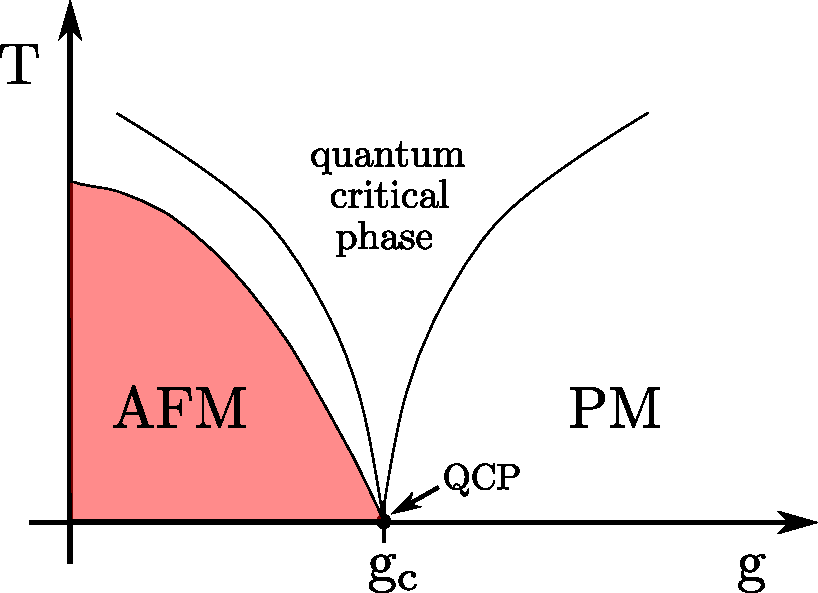
\includegraphics[width=0.7\textwidth]{phase_diagram.pdf}
	\caption{
This figure shows a schematic and simplified phase diagram for metals transition from a paramagnetic (PM) into an antiferrmagnetic (AFM) phase depending on a tunung parameter g.
The phase line of the AFM phase ends decreasing temperature down to $T = 0$ in a quantum critical point (QCP) at $\mt{g} = \mt{g}_{\mt{c}}$.
At this point the phase transition is only caused by quantum fluctuations.
At $T > 0$ thermal fluctuactions more and more dominates the phase transition.
Nevertheless quantum fluctuations influences the physical behaviour in a lagre regime, labeled as quantum critical phase.
	}
	\label{fig:phase diagram}
\end{figure}
%
Decreasing tempearutre the phase line between both magnetic phases reach a certain value for the tuning parameter g at $T = 0$, labeled with $\mt{g}_{\mt{c}}$.
This point is called quantum critical point and in comparsion with the phase transition at finite temperature quantum fluctuations are the origin of this phase transition.

Before starting with a qualitative derivation of the spin-fermion-model a short and rudimentary describtion of quantum phase transition is given.
This overview is required for the analytical discussion of our computation later.
However, the reason for phase transitions is always level crossing between the ground and an excited state.
Due to the fact that level crossing is forbidden a band gap $\Delta$ arises.
This band gap is therefore a characteristic energy scale of the quantum phase transition.
Considering only phase transitions of second order the characteristic energy scale $\Delta$ is proportional to the tuning parameter as
%
\begin{align}
	\Delta \sim \mt{J} |\mt{g} - \mt{g}_{\mt{c}}|^{z \nu},
	\label{eq:energy scale Delta}
\end{align}
%
where $z\nu$ is a critical exponent and J a energy scale of a microscopic coupling \cite{SachdevQCP}.
Beside a characteristic energy scale quantum phase transitions also possesses a characteristic length scale $\xi$, called correlation length, which diverges right at the quantum critical point.
%
\begin{align}
	\xi^{-1} \sim \Lambda |\mt{g} - \mt{g}_{\mt{c}}|^{\nu},
	\label{eq:correlation length xi}
\end{align}
%
where $\nu$ is again a critical exponent and $\Lambda$ an arbitrary inverse length scale like a momentum cut-off, for example.
Inserting \eqref{eq:correlation length xi} in \eqref{eq:energy scale Delta} yields a directly relation between both characteristic quantities.
For finite temperatures, $T > 0$, a second energy scale is given by $k_{\mt{B}} T$, where $k_{\mt{B}}$ is the Botzmann constant.
Comparing both energy scales yields a proportionality between temperatur and correlation length as
%
\begin{align}
	T \sim \xi^{-z}.
	\label{relation temperature and correlation length}
\end{align}
%
Further this explaines the curved conical boundary phase lines of the quantum critical phase in figure \ref{fig:phase diagram}.
In the case of small temperatures the critical exponent $z$ attains the value $z = 2$, so that the phase lines are shaped like a square root.
Increasing temperature the phase boundary lines are linear, since the critical exponent changing to $z = 1$ \cite{Patel&Sachdev}.
Inside this regime the physical behaviour of the metals is determined by quantum fluctions.

Knowing the physical origin of quantum phase transitions the spin-fermion-model can be introduced.
Instead of an microscopic and detailed mathematical describtion we want focus our introduction on qualitative arguments motivating the model.
The spin-fermion-model describes metals in the vicinity of a magnetic quantum critical point considering fermionic quasiparticles and bosonic spin density waves.
Thereby, the propagator is determined by the usual free fermionic Green function.
Spin fluctuations are constituted as collective modes and their propagator is characterized by the dynamical magnetic susceptibility.
%
\begin{align}
	\mathcal{D}_{\mu}(\vb{q}, \omega) = \sum\limits_{\vb{Q}} \frac{1}{(\vb{q}+\vb{Q})^{2} + \xi^{-2} - (\flatfrac{\omega}{v_{\mt{S}}})^{2}},
	\label{eq:undamped spin propagator}
\end{align}
%
where $\mu$ is the spatial direction of the spin density wave, $\xi$ the magnetic correlation length and $v_{\mt{S}}$ the spin wave velocity.
The spin wave velocity is of the same order as the Fermi velocity since spin fluctuations originate due to fermions in the vicinity of the Fermi surface.
Furthermore, the magnetic susceptibility possesses a peak at the momentum vector $\vb{Q} = (\pi, \pi)$.
This implicates a strong coupling interaction between momentum vectors $\vb{k}$ and $\vb{k} + \vb{Q}$.

Phase transitions are always associated by an order parameter equally the investigated antiferromagnetic phase transition, where the local magnetization measured by the spin expectation value $\expval{\vb{S}(\vb{r}_{i})}$ is the corresponding order parameter.
Naturally, we have to summerarize over all spins located at a certain position $\vb{r}_{i}$.
The order parameter is finite in the antiferromagnetic ordered phase and reaches zero in the paramagnetic disordered phase.
Further, the expectation value of the spin operator is spatially modulated according to $\expval{\mt{S}_{\mu}} \sim \exp({i\vb{Q}\vb{R}})$, where $\vb{R}$ is some lattice vector \cite{Weiss}, and therefore the order parameter and equally the propagator are periodical quantities.
In reciprocal space this is reflected in the periodicity  of the magnetic Brillouin zone spanned by the vector $\vb{Q}$.

Our describtion of the antiferromagnetic quantum phase transition in the spin-fermion-model is based on a few fundamental assumptions, comparatively to \cite{Abanov&Chubukov&Schmalian}.
We assume spin fluctuations arise over a large range of the tuning parameter and, futhermore, other low-energy collective degrees of freedom, independent on spin excitations, are neglectable.
Starting by large values of the tuning parameter g in the paramagnetic phase, the physical behaviour is described by Landau's Fermi liquid theory.
Decreasing the tuning parameter and getting closer to the quantum critical point changes the behaviour to a the Non-Fermi liquid.
Assuming only one type of fermions the arising collective modes are originated due to permanent interaction between particles and holes.
These bosonic spin excitations determine the physics in the vicinity of the quantum critical point and turning into smooth modes.
Therefore, we assume that only one dominant channel exist for fermion-fermion interaction with energies smaller than a certain energy cut-off $\Lambda$.
Further we introduce on collective spin mode which containts this interaction.

In the vicinity of the quantum critical point the (magnetic) correlation length $\xi$ and the coupling constant $\lambda$ diverges
Therefore the correlation length is much larger than the lattice constant, $\xi \gg a$, and the coupling constant is much larger than the band gap, $\lambda gg \Delta$, where the band gap as associated with the energy of spin excitations.
In the limit of large distance and small energies/temperatures a mircoscopic consideration of the lattice Hamiltonian is unnecessary.
In this low-energy theory spin fluctuations are described as a three component bosonic field $\Phi_{\mu}(\vb{x}, \tau)$ befined as a sum over all spin oparators analysed in the neighbourhood of the spin's site $i$, $\Phi_{\mu}(\vb{x}, \tau) \sim \sum_{i \in \Gamma(\vb{r}_{i})} \mt{S}_{\mu}(\vb{r}_{i})$, where $\mu$ is the spatial direction of the field and $\Gamma(\vb{r}_{i})$ represent the neighbourhood around the spin position $\vb{r}_{i}$ \cite{SachdevQCP}.
The magnitude of the bosnic field is chosen arbitrary and the field itself is considered as a real field.
The obtained effective Hamiltonian for the spin fluctuations in the low-energy theory is then given by
%
\begin{align}
	\mt{H}_{\Phi} &= 
	 	\sum\limits_{\mu} \int_{\vb{k}}\, \Big[
	 	-\frac{\vb{k}^{2}}{2} - \frac{r}{2}\Big] \Phi_{\mu}(\vb{k},\tau) \Phi_{\mu}(-\vb{k},\tau)
		+
		\frac{v_{\mt{S}}^{2}}{2} \pi_{\mu}(\vb{k},\tau) \pi_{\mu}(-\vb{k},\tau),
	\label{eq:Hamiltonian spin fluctuation}
\end{align}
%
where $r$ is a control parameter and corresponds to the squared inverse correlation length, $r = \xi^{-2}$.
The integral extends over the first Brillouin zone and the sum runs over the spatial direction of the bosonic field.

Further we have to take into account that the spin densiy waves are damped in consequence of the interaction with fermions.
The spin itself doesn't possess an own damping source.
The whole damping is governed by decaying of particel-holes-pairs and the full renormalized particel-hole bubble corresponds to the inverse lifetime of spin fluctuations.
The interation Hamiltonian between spin density waves and fermions is given by
%
\begin{align}
	\mt{H}_{\Psi\Phi} &= 
		-\lambda \sum\limits_{\mu} \int_{\vb{k}} \int_{\vb{q}}\,
		\Phi_{\mu}(\vb{k}-\vb{q}, \tau)
		\bigg[
			\Psi_{\mt{a}}^{\dag}(\vb{k},\tau) \cdot \sigma_{\mu} \cdot \Psi_{\mt{b}}(\vb{q},\tau)
			+
			\Psi_{\mt{b}}^{\dag}(\vb{k},\tau) \cdot \sigma_{\mu} \cdot \Psi_{\mt{a}}(\vb{q},\tau)
		\bigg],
	\label{eq:Hamiltonian interaction}
\end{align}
%
where $\lambda$ is the coupling constant, both integrals extend over the first Brillouin zone and the sum runs over all spatial directions of the bosonic field.
The index a and b at the fermionic fields $\Psi$ represent the two different Fermi surfaces in the obtained model which is explained below presently.
The imaginary part of the susceptibility has to be computed in the low-energy limit with the tools of the quantum field pertubation theory.
An explicite calculation is presented in the appendix \ref{app:particel-hole-bubble}.
Further, assuming the dynamic of the spin fluctuations is governed by the low-energy fermions the $\omega^{2}$-term in the susceptibility \eqref{eq:undamped spin propagator} is neglectable \cite{Abanov&Chubukov&Schmalian} and at the vicinity of the quantum critical point the correlation length diverges, so $\xi^{-2} \to 0$.
Then the damped magnetic susceptibility is then given by
%
\begin{align}
	\mathcal{D}_{\mu}(\vb{q}, i\omega_{n}) = \sum\limits_{\vb{Q}} \frac{1}{(\vb{q}+\vb{Q})^{2} + \gamma|\omega_{n}|},
	\label{eq:undamped spin propagator}
\end{align}
%
where $\omega_{n}$ represent the bosonic Matsubara frequency.
Due to the fact that damping of spin fluctuations is strongly connected to fermions their are no independent degrees of freedom.
The damped susceptibility constitutes the interaction between fermions on the Fermi surface seperated by the large vector $\vb{Q}$.
These points on the Fermi surface are labeled as hot-spots in two dimensions, which we want to discuss next.
%
\begin{figure}
	\centering
	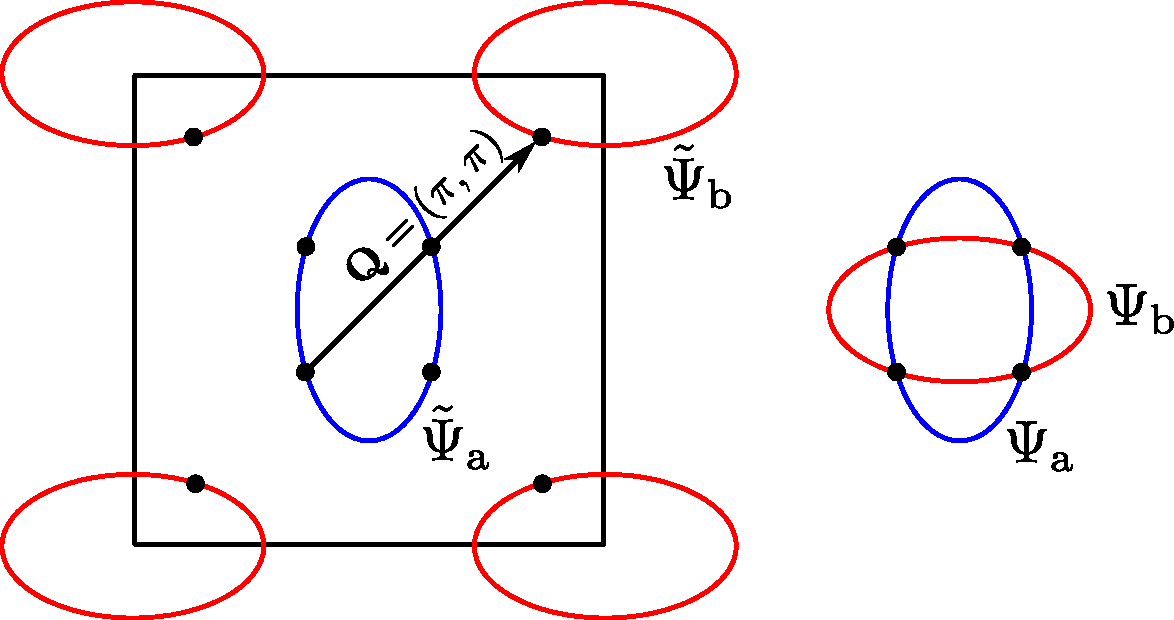
\includegraphics[width=0.7\textwidth]{hotspots.pdf}
	\caption{
One the left hand side the Brillouin zone is depicted containing the Fermi surface of both species of fermions, $\tilde{\Psi}_{\mt{a}}$ and $\tilde{\Psi}_{\mt{b}}$.
While the fermions $\tilde{\Psi}_{\mt{a}}$ are located with an anisotropic parapolical dispersion at the origin $(0,0)$, the fermions $\tilde{\Psi}_{\mt{b}}$ are located with a $\flatfrac{\pi}{2}$-rotated anisotropic parapolical dispersion at the corners of the Brillouin zone, $(\pi,\pi)$ for example.
The vector $\vb{Q}$ connects certain points on the Fermi surface, called hotspots and represented with dots. 
As a result of this an attraction between these fermions occurs.
On the right hand side the fermions $\tilde{\Psi}_{\mt{a}}$ are shifted to the corner at $(\pi,\pi)$.
The convienence of this represantation is that the coupling between fermions and spin fluctuations is local and independent of the position.
	}
	\label{fig:hotspots}
\end{figure}
%
In comparison to a normal metals these new interaction of spin fluctuations seperates the Fermi surface in "hot" and "cold" manifolds.
Considering a point $\vb{k}$ on the Fermi surface of a $d$-dimensional system, so the fermion has zero energy.
The spin density wace connects this point to another point $\vb{k}+\vb{Q}$.
We require that this point has to be also on the Fermi surface, which is our second constraints.
Both contraints yield a $d-2$-dimension manifold for a $d$-dimensional system.
In the case of $d=2$ the "hot" manifold is called a hot-spot.
Another visualization of "hot" manifolds offers the magnetic Brillouin zone spanned by the vector $\vb{Q}$.
The intersections of the magnetic Brilouin zone and the Fermi surface are eauivalent to the "hot" manifolds.

In our investigated model the fermions are considered as free up to the interaction with the spin fluctuations.
We assume two species of fermions, $\tilde{\Psi}_{\mt{a}}$ and $\tilde{\Psi}_{\mt{b}}$, with an anisotropic parabolic dispersion, as suggested in \cite{Patel&Sachdev} and depicted on the left hand side in figure \ref{fig:hotspots}.
This isn't a discrepancy to our previous constraint, assuming one fermion since both species of fermions are electrons and differ only in their dispersion.
The fermions $\tilde{\Psi}_{\mt{a}}$ and $\tilde{\Psi}_{\mt{b}}$ are located on an ellipse around the origin $(0,0)$ and $(\pi,\pi)$, respectivily.
Both ellipses are seperated by the vector $\vb{Q} = (\pi,\pi)$ and rotated by $\flatfrac{\pi}{2}$ to each other.
For achieving a continuum theory the ellipse centered around $(\pi,\pi)$ is shifted by the vector $\vb{Q}$ to the origin.
Therefore new fermionic fields, $\tilde{\Psi}_{\mt{a}}(\vb{r}) = \Psi_{\mt{a}}(\vb{r})$ and $\tilde{\Psi}_{\mt{b}}(\vb{r}) = \Psi_{\mt{b}}(\vb{r}) \exp(i\vb{Q}\vb{r})$, are introduced.
The new dispersion of the fermions $\Psi_{\mt{a}}(\vb{r})$ and $\Psi_{\mt{b}}(\vb{r})$ is depicted on the right hand side in figure \ref{fig:hotspots}
The enormous advantage is that the coupling between the fermions caused by spin density waves is local and indipendent of the position.
In reciprocal space, the free continuum Hamiltonian of the fermions $\Psi_{\mt{a}}(\vb{r})$ and $\Psi_{\mt{b}}(\vb{r})$ is given by
%
\begin{align}
	\mt{H}_{\Psi} &= 
	 	\int_{\vb{k}}\,
	 	\bigg[
	 		\epsilon_{\mt{a}}(\vb{k})
	 		\psi_{\mt{a}}^{\dag}(\vb{k},\tau)
	 		\psi_{\mt{a}}(\vb{k},\tau)
	 		+
	 		\epsilon_{\mt{b}}(\vb{k})
	 		\psi_{\mt{b}}^{\dag}(\vb{k},\tau)
	 		\psi_{\mt{b}}(\vb{k},\tau)
	 	\bigg],
	 \label{eqHamiltonian electrons}
\end{align}
%
where the intergal extends over the first Brillouin zone and $\epsilon_{\mt{a}}(\vb{k})$ and $\epsilon_{\mt{b}}(\vb{k})$ are the anisotropic parabolical dispersions, corresponding to the fermion species a and b, given by
%
\begin{align}
	\epsilon_{\mt{a}}(\vb{k}) = \frac{k_{x}^{2}}{2m_{1}} + \frac{k_{y}^{2}}{2m_{2}} - \mu_{0}
	\qq{and}
	\epsilon_{\mt{a}}(\vb{k}) = \frac{p_{x}^{2}}{2m_{2}} + \frac{p_{y}^{2}}{2m_{1}} - \mu_{0},
	\label{eq:dispersion relations}
\end{align}
%
where $\mu_{0}$ is the chemical potential.
%
%
\section{Prove of Momentum Conservation and Breaking Translation Symmetry by Umklapp Scattering}
\label{sec:umklapp scattering}
%
%



















 %done
%
\cleardoublepage
%
%
%
\chapter{Static Conductivity in the Spin Fermion Model considering Umklapp Scattering}
\label{ch:calculation}
%
%
%
The static electrical conductivity $\sigma_{\mt{dc}}$ is computed in this chapter, using the memory-matrix-formalsim.
The underlying model is the spin-fermion-model (see chapter \ref{ch:spin fermion model}), including umklapp scattering that breaks translation symmetry.
In this chapter, our focus lies on the physical analysis of the obtained expression for the conductivity.
An explicite computation is demonstrated in appendix \ref{appch:static susceptibility} and \ref{appch:green function}.

%
%
%\section{Static Conductivity's Derivation}
%\label{sec:deviation conductivity}
%
%
Two physical objects, fermions near the Fermi surface and spin fluctuations, are considered in the spin-fermion-model as introduced in the previous chapter.
Spin fluctuations are generated at the vicinity of an antiferromagnetic quantum critical point due to particle-holes-excitations.
Fermions, located at the point $\vb{k}$ and $\vb{k}+\vb{Q}$ on the Fermi suface, are connected to each other because of these fluctuations.
The momentum conservation of the spin-fermion-model Hamiltonian has been shown in the previous chapter.
The static electrical conductivity is thus infinite as it is poven in chapter \ref{ch:infinite conductivity}.
Considering umklapp scattering, the translation symmetry is broken and the momentum is unconserved.
As a conseuqence the static conductivity becomes finite.
This calculation is presented here.

The memory-matrix-formalism is used in chapter \ref{ch:memory matrix formalism} to derivate the following formula for the static electrical conductivity, including the spin-fermion-model as well as umklapp scattering.
%
\begin{align}
	\sigma_{\mt{dc}} = \lim\limits_{z \to 0} \frac{z \cdot |\chi_{\mt{JP}}(\omega = 0)|^{2}}{\mathcal{G}_{\dot{\mt{P}}\dot{\mt{P}}}(\vb{k}, z)}
	\label{eq:static conductivity formula}
\end{align}
%
Here, $z$ is a complex frequency and $\chi_{\mt{JP}}(\omega = 0)$ is the static susceptibility between current and momentum.
The Green function in the denominator is given by
%
\begin{align}
	\mathcal{G}_{\dot{\mt{P}}\dot{\mt{P}}}(\vb{k}, z) = \int\limits_{0}^{\infty} \dd{t} e^{izt} \expval{\comm{\dot{\mt{P}}(t)}{\dot{\mt{P}}(0)}_{-}}_{0},
	\label{eq:Green function}
\end{align}
%
where the usual quantum mechanical commutator is used, indicated with the minus sign at the squared brackets.
The expectation value is evaluated with respect to the unpertubative Hamiltonian H, visualized with the index 0.
The interaction between fermions and spin fluctuations is included in the Hamiltonina H.
The time derivative of momentum is given by equation \eqref{eq:time derivative momentum finite}.

The possible temperature dependence of the Green function $\mathcal{G}_{\dot{\mt{P}}\dot{\mt{P}}}(\vb{k}, z)$ and the static susceptibiliy $\chi_{\mt{JP}}(\omega = 0)$ is investigated.
The latter is expected to be temperature independent.
This calculation is shown in detail in the appendix \ref{appch:static susceptibility}, using the diagrammatic pertubation technique.
The considered diagrams are the electron-pair bubble for each species of fermions, depicted in figure \ref{fig:static susceptibility}.
Therefore, the obtained expression of the susceptibility is given by
%
\begin{align}
	\chi_{\mt{PJ}}(\omega = 0) = \frac{\sqrt{m_{1} m_{2}}}{\pi} T \cdot \ln(e^{\flatfrac{\mu}{T}} + 1),
	\label{eq:static susceptibility computed}
\end{align}
%
where the chemical potential is denoted as $\mu$.
The logarithm is approximated in the limit of small temperatures ($\mu \gg T$) to $\ln(e^{\flatfrac{\mu}{T}} + 1) \rightarrow \flatfrac{\mu}{T}$.
The temperature cancels when this expression is inserted and the static susceptibility is given by constant parameters, $\chi_{\mt{PJ}}(\omega = 0) = \flatfrac{\mu\sqrt{m_{1} m_{2}}}{\pi}$.
The chemical potential is assumed to be temperature independent in the observed regime.

%
\begin{figure}
	\centering
	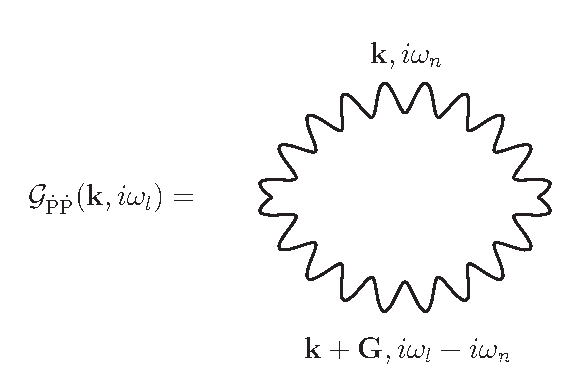
\includegraphics[width=0.4\textwidth]{spin_wave_bubble.eps}
	\caption{
The zeroth order bubble diagram is shown for spin density fluctuations.
The wavy lines symbolizes the spin density wave, denoted as $\mathcal{D}_{\mu}(\vb{k},i\omega_{n})$.
The momentum of lower line is modified by the vector $\vb{G}$, originated from umklapp scattering.
	}
	\label{fig:spin wave bubble}
\end{figure}
%
The only temperature dependence of the static electrical conductivity emerges hence by the Green function $\mathcal{G}_{\dot{\mt{P}}\dot{\mt{P}}}(\vb{k}, z)$.
Only the free bubble diagram is considered when calculating the Green function with diagrammatic pertubation theory, which is depicted in figur \ref{fig:spin wave bubble}.
Higher order terms in the diagrammatic treatment are corrections of the bubble diagram.
Therefore the conductivity or resistance is only determined by spin fluctuations.
Resistance is a consequence of fermionic coupling to other degrees of freedom, obtained as finite fermionic lifetime.
It is thus proportional to the imaginary part of the retarded Green function $\mathcal{G}_{\dot{\mt{P}}\dot{\mt{P}}}^{\mt{ret}}(\vb{k}, z)$.
Appendix \ref{appch:green function} shows the detailed computation of the expression of the retarded Green function.
%
\begin{align}
	\Im{\mathcal{G}_{\dot{\mt{P}}\dot{\mt{P}}}^{\mt{ret}}(\vb{k}, \omega)} &= 
		-\frac{4 \gamma^{2} \beta \omega}{\pi}
		\sum\limits_{\vb{Q}_{1}, \vb{Q}_{2}}
		\sum\limits_{\vb{G}}
		\vert \mt{J}_{\vb{G}} \vert^{2}
		\int\limits_{0}^{\infty} \dd{\epsilon}
		\frac{\epsilon^{2} e^{\beta \epsilon}}{(e^{\beta \epsilon} - 1)^{2}}
		\notag \\
		&\times
		\int_{\vb{k}} G_{j}^{2} \cdot
		\frac{1}{(\vb{k}+\vb{G}-\vb{Q}_{1})^{4} + \gamma^{2} \epsilon^{2}} \cdot
		\frac{1}{(\vb{k} + \vb{Q}_{2})^{4} + \gamma^{2} \epsilon^{2}}
\end{align}
%
The integral is extended over the first Brillouin zone.
The periodicity of the spin susceptibility and pertubation is considered by the sums over $\vb{Q}_{i}$ ($i=1,2$) and $\vb{G}$, respectivily.
In both cases these are reciprocal lattice vectors.
Spatial direction of the momentum is represented by the index $j$ and $\beta^{-1} = T$.
The obtained integrals are now investigated with respect to different cases since their are not exactly solvable.
%
%
%\section{Analysis of the static conductivity}
%\label{sec:analysis conductivity}
%
%

The intergal converges if the magnitude of one of the momentum terms, $\vb{k}+\vb{G}-\vb{Q}_{1}$ or $\vb{k} + \vb{Q}_{2}$, is large.
Since both terms are of the power of four, the integral is a fast decreasing function in the large momentum limit.
The integral diverges, if these terms are zero and this happens in many constellations.
One of the most divergent one is assumed in the following approach.
The vector $\vb{k}$ is limited to the first Brillouin zone and the reciprocal lattice vectors are set to $\vb{G} = \vb{Q}_{1}$ and $\vb{Q}_{2} = 0$.
The choice of the reciprocal lattice vectors is arbitrary and it is therefore possible that the $j$-component of $\vb{G}$ is large.
This divergence is killed by the coupling parameter $\mt{J}_{\vb{G}}$ that is assumed to be fast decreasing for large $|\vb{G}|$.

The remaining momentum integral is now exactly integrable.
First of all, the momentum and frequency variables are transformed into dimensionles variables, using the transformation rules $\vb{k} = \vb{y} \cdot \sqrt{\gamma T}$ and $\epsilon = x \cdot T$, respectivily.
The new variable $\vb{y}$ is further transformed into plane polar coordinates.
The upper limit of the radius $|\vb{y}|$ is set to infinity, since the integrand is decreasing fast to zero for $|\vb{y}| \to \infty$.
As a consequence the angular integral is easily evaluated, yielding the factor $2\pi$.
The remaining integral is given by the following expression.
%
\begin{align}
	\Im{\mathcal{G}_{\dot{\mt{P}}\dot{\mt{P}}}^{\mt{ret}}(\vb{k}, z)} = 
		 -\frac{2 \cdot G_{j}^{2} \cdot \vert \mt{J}_{\vb{K}} \vert^{2}}{\gamma \cdot \pi^{2}} \cdot \frac{\omega}{T}
		\int\limits_{0}^{\infty} \dd{x}
		\frac{x^{2} e^{x}}{(e^{x} - 1)^{2}}
		\int\limits_{0}^{\infty} \dd{y}
		\frac{y}{\big(y^{4} + x^{2}\big)^{2}}
\end{align}
%
The $y$-integral is substituted one last time, using the transformation rule $y^{2} = z \cdot x$.
The obtained integral is evaluated to $\flatfrac{\pi}{4}$, using the integral formula \eqref{eq:integral1}.
Both limits, $x \to 0$ and $x \to \infty$, of the intergal over $x$ are investigated.
In the case of large $x$, the integral is decreasing fast to zero due to the ratio of the exponential functions.
The upper limit is thus set to one and the integrand is expanded for small values of $x$.
In first order the integrand is approximated to $\flatfrac{1}{x^{3}}$.
This is a highly divergent function in the limit $x \to 0$ and as a consequence the static conductivity is divergent as well.

The result of a divergent conductivity is surely incorrect in a system with broken translation symmetry.
In chapter \ref{ch:infinite conductivity}, it is shown that translation symmetry and the consequent conserved momentum causes an infinite conductivity in the static limit.
Chapter \ref{ch:spin fermion model} shows, that momentum is conserved in the unpertubated spin-fermion-model \eqref{eq:time derivative momentum}, while it is unconserved considering umklapp scatering \ref{eq:time derivative momentum finite}.
As a concequence, a finite static conductivity is expected instead of divergence.

The origin of this discrepancy is supposed to be in the choice of the control parameter $r$.
The paramter $r$ is assumed to be zero, since its proportional to $\xi^{-2}$ and the correlation length $\xi$ diverges at the quantum critial point.
This assumption is incorrect in the sence that the system is not directly at the quantum cirtical point, but rather in the vicinity of him.
The system is supposed to be in the quantum critical phase, see figure \ref{fig:phase diagram}, at a point with tuning parameter $\mt{g} = \mt{g}_{\mt{c}}$ and temperature $ T > 0$.
While the temperature is decreased to get closer to the quantum critical point, the tuning parameter is fixed.
Considering a finite value of the control parameter $r$, the imaginary part of the retareded Green function is given by
%
\begin{align}
	\Im{\mathcal{G}_{\dot{\mt{P}}\dot{\mt{P}}}^{\mt{ret}}(\vb{k}, z)} &= 
		-\frac{4 \gamma^{2} \beta \omega}{\pi}
		\sum\limits_{\vb{Q}_{1}, \vb{Q}_{2}}
		\sum\limits_{\vb{G}}
		\vert \mt{J}_{\vb{G}} \vert^{2}
		\int\limits_{0}^{\infty} \dd{\epsilon}
		\frac{\epsilon^{2} e^{\beta \epsilon}}{(e^{\beta \epsilon} - 1)^{2}}
		\notag \\
		&\times
		\int_{\vb{k}} G_{j}^{2} \cdot
		\frac{1}{((\vb{k}+\vb{G}-\vb{Q}_{1})^{2} + r)^{2} + \gamma^{2} \epsilon^{2}} \cdot
		\frac{1}{((\vb{k} + \vb{Q}_{2})^{2} + r)^{2} + \gamma^{2} \epsilon^{2}}
\end{align}
%
The approach to solve the integrals is nearly the same as above.
Firstly, the convergence of large values of momenta is not changed, because of considering $r$.
One of the most divergent constellations is stil $\vb{G} = \vb{Q}_{1}$ and $\vb{Q}_{2} = 0$.
The divergence, generated by large values of $G_{j}$, is still killed since the coupling parameter $\mt{J}_{\vb{G}}$ decreases fast in the limit $|\vb{G}| \to \infty$.
The remaining momentum integral is of the same structure as above and exactly solvable.
Therefore, the momentum integral is firstly transformed into plane polar coordinates, $\vb{k} = (k\cos\phi, k\sin\phi)$.
The upper limit of $k$ is again set to infinity, since the integrand decreases fast to zero for $k \to \infty$ and the contributions are neglectaed.
%
\begin{align}
	\Im{\mathcal{G}_{\dot{\mt{P}}\dot{\mt{P}}}^{\mt{ret}}(\vb{k}, z)} &= 
		-\frac{\vert \mt{J}_{\vb{G}} \vert^{2} \cdot G_{j}^{2}}{\gamma \pi^{2}} \cdot 
		\frac{\omega}{T}
		\int\limits_{0}^{\infty} \dd{\epsilon}
		\frac{\epsilon^{2} e^{\beta \epsilon}}{(e^{\beta \epsilon} - 1)^{2}}
		\int\limits_{0}^{\infty} \dd{k}
		\frac{k}{((r + k^{2})^{2} + \gamma^{2} \epsilon^{2})^{2}}
	\label{eq:starting expression}
\end{align}
%
The angular integral is already performed and the obtained momentum integral is substituted using $z = \flatfrac{(r + k^{2})}{\gamma\epsilon}$.
In comparison to the case above, the lower limit is changed to $\flatfrac{r}{\gamma \epsilon}$.
Both cases are equivalent in the limit $r \to 0$.
The finite lower boundary guarantees the convergence of the remaining integral over $\epsilon$.
The integral over $z$ is performed, utilizing the integral formula \eqref{eq:integral1} again.
The dimensionless variable are introduced, using $x = \beta \epsilon$.
The obtained expression is given by
%
\begin{align}
	\Im{\mathcal{G}_{\dot{\mt{P}}\dot{\mt{P}}}^{\mt{ret}}(\vb{k}, z)} &= 
		-\frac{\vert \mt{J}_{\vb{G}} \vert^{2} \cdot G_{j}^{2}}{4 \gamma \pi^{2}} \cdot 
		\frac{\omega}{T}
		\notag \\
		\times &\int\limits_{0}^{\infty} \dd{x}
		\frac{1}{x} \frac{e^{x}}{(e^{x} - 1)^{2}} \cdot
		\bigg[\pi - \frac{2 \flatfrac{\tilde{r}}{x}}{(\flatfrac{\tilde{r}}{x})^2 + 1} - 2 \arctan(\flatfrac{\tilde{r}}{x})\bigg],
	\label{eq:figure behaviour integrand}
\end{align}
%
where the abbreviation $\tilde{r} = \flatfrac{r}{\gamma T}$ is introduced.
The integral over $x$ is not analytical exactly solvable.
However, the integral is finite in both limits, $x \to 0$ and $x \to \infty$.
The latter is surely statisfied due to the ratio of exponential functions is fast decreasing to zero and no other term is divergent.
In the limit $x \to 0$, the integrand is limited by $\flatfrac{4}{3\tilde{r}^{3}}$, which is only divergent for $\tilde{r} \to 0$.
The behaviour of the integrand is depicted on left hand side in figure \ref{fig:behaviour integrand}, where $\tilde{r} = 2$.
%
\begin{figure}[t]
	\centering
	\subfigure[Behaviour of the integrand in \eqref{eq:figure behaviour integrand}]{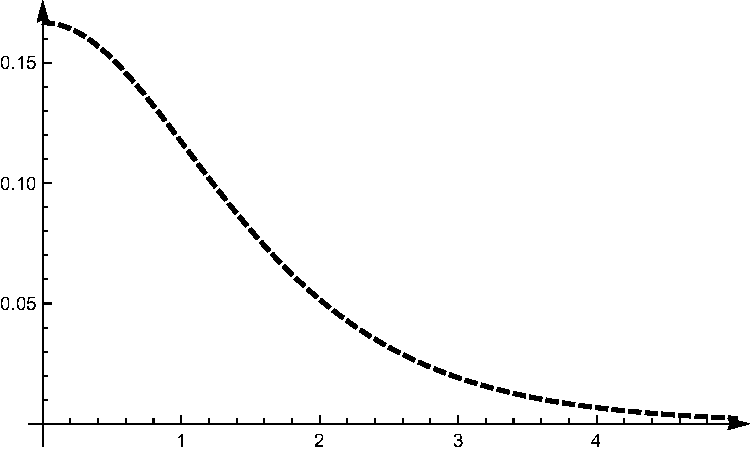
\includegraphics[width=0.49\textwidth]{behaviour_integrand.pdf}}
	\subfigure[Power dependence of the squared brackets multiplied by $\flatfrac{1}{x^{3}}$ in \eqref{eq:figure behaviour integrand}]{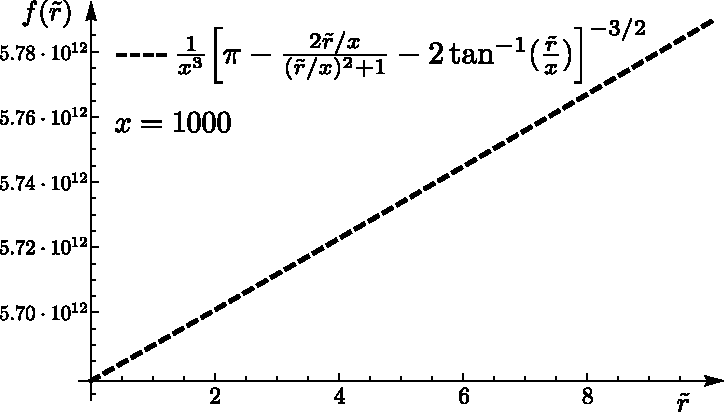
\includegraphics[width=0.49\textwidth]{dependence_integrand.pdf}}
	\caption{
On the left hand side, the behaviour of the integrand in equation \eqref{eq:figure behaviour integrand} is depicted for large und small values of $x$, where the factor $\tilde{r} = \flatfrac{r}{\gamma T}$ is set to 2.
The integrand function is convergent for large values due to the function decreases fast for large values of $x$.
For small values of $x$, the function takes a constanst value of $\flatfrac{4}{3\tilde{r}^{3}}$.
The integrand gets more divergent for small $x$, if the value $\tilde{r}$ decrease to zero.
The power dependence of the obtained momentum integral in \eqref{eq:figure behaviour integrand} is depicted on the right hand side, where $x=1000$.
Since the behaviour is linear, the investigated expression has the power of $-\flatfrac{3}{2}$.
	}
	\label{fig:behaviour integrand}
\end{figure}
%
A solution of the integral is evaluated determining the behaviour of the expression in squared brackets.
For large values of $x$, a linear $r$-dependence is given by the power of $-\flatfrac{3}{2}$.
This is depicted in the right hand side of figure \ref{fig:behaviour integrand}, where $x$ is set to $1000$.
An approximated expression is generated for the interand using the method of power counting.
The initial point of this approach is the momentum integral in euqtion \eqref{eq:starting expression}.
Numerator and differential yield in total the power of two, while the denominator generates the power of eight.
The integrand is a function proportional to $k^{-6}$ combing both powers.
The further approach is to investigate singularities of the integrand.
The limit $r \to 0$ or $\epsilon \to 0$ is seperately generated singularities in the function.
Both are considered with the power of three, since the power of them is half in comparison to the power of $k$ in equation \eqref{eq:starting expression}.
The integrand is therefore approximated by the following expression.
%
\begin{align}
	\Im{\mathcal{G}_{\dot{\mt{P}}\dot{\mt{P}}}^{\mt{ret}}(\vb{k}, z)} &\approx 
		-\frac{2 \vert \mt{J}_{\vb{G}} \vert^{2} \cdot G_{j}^{2}}{\gamma \pi^{2}} \cdot 
		\frac{\omega}{T}
		\int\limits_{0}^{\infty} \dd{x}
		\frac{x^{2} e^{x}}{(e^{x} - 1)^{2}}
		\frac{1}{(\tilde{r}^{2} + x^{2})^{\flatfrac{3}{2}}}
\end{align}
%
In figure \ref{fig:integrand exact vs approx}, the approximated expression is illustrated against the exact one.
The behaviour of both are nearly identical and the estimation is inspected to be valid.
The integrand decreases still fast to zero for $x \to \infty$, while the upper limit is set to some arbitrary cut-off $\Lambda$.
%
\begin{figure}[t]
	\centering
	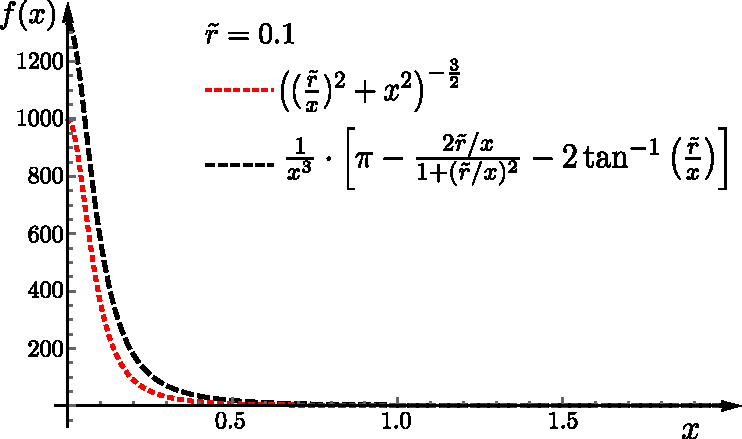
\includegraphics[width=0.6\textwidth]{original_vs_powercounting.pdf}
	\caption{
This figure shows the obtained expression of the momentum intgeral calculation (black curve, large strokes) in contrast to the obtained approximation using power counting technique (red curve, small strokes).
The used approximation is considered as good, since the characteristic of both curves is quite similar.
The value of $\tilde{r}$ is set to $0.1$.
	}
	\label{fig:integrand exact vs approx}
\end{figure}
%
The ratio of the exponential functions are then expanded for small values of $x$ up to the first non-vanishing order.
The remained integral is solved exactly while the solution of its is expanded for small $\flatfrac{\tilde{r}}{\Lambda}$.
%
\begin{align}
	\Im{\mathcal{G}_{\dot{\mt{P}}\dot{\mt{P}}}^{\mt{ret}}(\vb{k}, z)} &\approx 
		-\frac{2 \gamma \vert \mt{J}_{\vb{G}} \vert^{2} \cdot G_{j}^{2}}{\pi^{2} \Lambda} \cdot \frac{\omega T}{r^{2}}
\end{align}
%
To get the static electrical conductivity, this expression and the  approximated value of \eqref{eq:static susceptibility computed} is inserted into equation \eqref{eq:static conductivity formula}.
%
\begin{align}
	\sigma_{\mt{dc}}(T) = \frac{\mu\: m_{1}\: m_{2}\: \Lambda}{2\: \gamma\: \vert \mt{J}_{\vb{G}} \vert^{2}\: G_{j}^{2}} \cdot \frac{r^{2}}{T}
\end{align}
%
Beside the temperature itself, the only temperature dependent parameter is the control parameter $r$, which is proportional to the squard inverse correlation length, $r = \xi^{-2}$.
The correlation length is originated due to the fact that the system possesses a quantum phase transition and is temperature dependent is given by $\xi = T^{-1/z}$, as shown in chapter \ref{ch:spin fermion model}.
$z$ is a critical exponent and it is chosen in dependence of the temperature distance to the qantum critical point.
The corresponding temperature depencence of the control parameter is provided to $r = T^{2/z}$.
The resistance is determined by the inverse of the conductivity.
Considering only the temperature dependent parameters, the static resistance is given by
%
\begin{align}
	\rho_{\mt{dc}}(T) \sim T^{1-\flatfrac{4}{z}}.
	\label{eq:solution resistance}
\end{align}
%
Two possible choices are mentioned for the ciritcal exponent $z$.
In the vicinity of the quantum critical point at higher temperatures, $z$ is chosen to be one.
The $T$-dependence of the resistance is then given by $T^{-3}$.
In the limit $T \to 0$, this is highly divergent.
$z$ can be chosen to be 2 for lower temperatures.
Nevertheless, the $T$-dependence is evaluated to $T^{-1}$, which is still divergent in the limit $T \to 0$.

Our physial expectation is not confirmed with this divergent behaviour of the resistance.
Experiments of observed metals \cite{Loehneysen} are shown a linear temperature dependence of the resistance, $\rho(T) = \rho_{0} + A\: T$.
The behaviour of the resistance is therefore described incorrect using the obtained solution \eqref{eq:solution resistance}.
A possible origin of this disgrepancy between experiemnt and theory is maybe the diagrammatic pertubation theory.
In equation \eqref{eq:Green function}, the time evolution operator is expanded up to the first non-vanishing order.
This yields the free bubble diagram, while correction to the bubble are considered if the time evolution operator is expanded up to the next order.







%In Landau's Fermi liquid theory the resistance of a metal is given by $\rho(T) = \rho_{0} + A\: T^{2}$, where the residual resistance due to impurity scattering is represented by $\rho_{0}$.
%The $T^2$-dependence is originated by electron-electron scattering and umklapp-scattering \cite{Bader, Pal}


%In \cite{Loehneyesen} metals are investigated where a non-Fermi liquid behaviour 
%The consideration of umklapp scattering 

%Both results do not describe the physical results, presented in \cite{Loehneysen}.
%Here, 

%coincide 


















 %done
%
\cleardoublepage
%
%
%
\chapter{Memory-Matrix-Formalism}
\label{ch:memory matrix formalism} 
%
%
%
The memory-matrix-formalism is a technique to determine the correlation function between two observables.
In difference to other methods the Liouville space is considered.
The derivation of the memory-matrix-formalism is exhaustively demonstrated in this chapter, as suggested in \cite{Forster}.
At the beginning Kubo's relaxation function is introduced, since the correlation function is based on it in memory-matrix-formalism.
After the derivation the formula for the static electrical conductivity is determined for the spin-fermion-model pertubated by umklapp scattering.
%
%
\section{Kubo relaxation function}
\label{sec:kubo relaxation function}
%
%
A system in equlibrium, represented by the Hamiltonian $\mt{H}_{0}$, is considered.
The pertubation $\mt{H}_{1} = -\mt{B} \cdot F(t)$ is switched on at an arbitrary time $t'$.
The coupling to the system is determined by the operator B and the time evolution of the pertubation is described by $F(t)$, where $F(t)$ is assumed to be zero for times $t<t'$.
Our interest is now focused on the reaction of an operator A due to the pertubation.
The deviation in comparing to the equilibrum value is given by
%
\begin{align}
	\delta\expval{\mt{A}(t)} := \expval{\mt{A}}(t) - \expval{\mt{A}(t)}_{H_{0}} \approx \int\limits_{-\infty}^{\infty} \dd{t'} \chi_{\mt{AB}}(t-t') F(t')
	\label{eq:Kubo formula}
\end{align}
%
where $\chi_{\mt{AB}}(t-t')$ is called the retarded susceptibility and is given by
%
\begin{align}
	\chi_{\mt{AB}}(t-t') = i \Theta(t-t') \expval{\comm{\mt{A}_{\mt{I}}(t-t')}{\mt{B}_{\mt{I}}(0)}}_{\mt{H}_{0}}
	\label{eq:dynamical susceptibilty}
\end{align}
% 
The above equation for $\delta\expval{\mt{A}(t)}$ is denoted as the Kubo formula.
In the following, a certain type of pertubations is considered.
The time evolution of the pertubation is assumed to be $F(t) = \Theta(-t) \cdot F \cdot e^{-s\tau}$.
The pertubation is switched on adiabatically at $t = -\infty$ and is switched off at $t=0$.
This time evolution is inserted into the Kubo formula and $t-t'$ is substituted by $\tau$.
The deviation of $\mt{A}(t)$ is then given by $\delta\expval{\mt{A}(t)} = \Phi_{AB}(t) \cdot F e^{st}$.
The arising function $\Phi_{\mt{AB}}(t)$ is called Kubo relaxation function and is given by
%
\begin{align}
	\Phi_{\mt{AB}}(t) = \frac{i}{\hbar} \lim\limits_{s \to 0} \int\limits_{t}^{\infty} \dd{\tau} \expval{\comm{\mt{A}_{\mt{I}}(\tau)}{\mt{B}_{\mt{I}}(0)}}_{0} e^{-s\tau}.
	\label{eq:Kubo relaxation function}
\end{align}
%
The lower limit of the integral is determined to $t$ due to the $\theta$-distribution.
For a more detailed derivation of the Kubo relaxation function see \cite{Schwabl} or \cite{Schwabl2}.
Between the Kubo relaxation function and the Kubo formula exist three very important relations used during the derivation of the correlation function and the formula of the conductivity.
%
\begin{enumerate}
	\item $\begin{aligned}[t] \chi_{\mt{AB}}(t) = -\Theta(t) \dv{t} \Phi_{\mt{AB}}(t) \end{aligned}$\hfill \refstepcounter{equation}(\theequation)\label{eq:relation 1 between Phi and chi}
	\item $\begin{aligned}[t] \Phi_{\mt{AB}}(t = 0) = \chi_{\mt{AB}}(\omega = 0) \end{aligned}$\hfill \refstepcounter{equation}(\theequation)\label{eq:relation 2 between Phi and chi}
	\item $\begin{aligned}[t] \Phi_{\mt{AB}}(\omega) = \frac{1}{i\omega}\big[\chi_{\mt{AB}}(\omega) - \chi_{\mt{AB}}(\omega = 0)\big]. \end{aligned}$\hfill \refstepcounter{equation}(\theequation)\label{eq:relation 3 between Phi and chi}
\end{enumerate}
%
The evidence of these tree relations are shown in the appendix \ref{app:properties of the Kubo relaxation function}.
The Kubo relaxation function is now transfered into a commutator independent form, using two identies.
The first identity is given by
%
\begin{align}
	\expval{\comm{\mt{A}(t)}{\mt{B}(t')}} &= \frac{1}{Z} \Tr{\comm{\rho}{\mt{A}(t)} \mt{B}(t')},
	\label{eq:identity expectation value}
\end{align}
%
where the invariance of the trace with respect to cycling permutation is used.
The second identity is denoted as the Kubo-identity.
%
\begin{align}
	i \comm{\rho}{\mt{A}(t)} &= i \Big[\rho \mt{A}(t) - e^{-\beta H} e^{\beta \mt{H}} \mt{A}(t) e^{-\beta \mt{H}}\Big]
	\notag \\
	\Leftrightarrow\ i \comm{\rho}{\mt{A}(t)} &= -i \rho \int\limits_{0}^{\beta} \dd{\lambda} \dv{\lambda} e^{\lambda \mt{H}} \mt{A}(t) e^{-\lambda \mt{H}}
	\notag \\
	\Leftrightarrow\ i \comm{\rho}{\mt{A}(t)} &= -i \rho \int\limits_{0}^{\beta} \dd{\lambda} \comm{\mt{H}}{\mt{A}(t-i\lambda)}
	\notag \\
	\Leftrightarrow\ i \comm{\rho}{\mt{A}(t)} &= -\rho \int\limits_{0}^{\beta} \dd{\lambda} \dot{\mt{A}}(t-i\lambda)
	\label{eq:Kubo-identity}
\end{align}
%
Here the analogy between the time evolution of an operator and the exponential function is used in the second step.
Furthermore, Heisenberg equation of motion is utilied in the third step.
The time derivative of the operator A is symbolizied with the dot above the operator.
%
\begin{align}
	&\Phi_{\mt{AB}}(t) = -\lim\limits_{s \to 0} \int\limits_{0}^{\beta} \dd{\lambda} \int\limits_{t}^{\infty} \dd{\tau} \expval{\dot{\mt{A}}_{\mt{I}}(\tau-i\lambda\hbar) \mt{B}_{\mt{I}}(0)}_{0} e^{-s\tau}
	\notag \\
	\overset{\mt{PI}}{\Leftrightarrow}\ &\Phi_{\mt{AB}}(t) = \int\limits_{0}^{\beta} \dd{\lambda} \expval{\mt{A}_{\mt{I}}(t-i\lambda\hbar) \mt{B}_{\mt{I}}(0)}_{0} = \int\limits_{0}^{\beta} \dd{\lambda} \expval{\mt{A}_{\mt{I}}(t) \mt{B}_{\mt{I}}(i\lambda\hbar)}_{0}
	\label{eq:Kubo relaxation function 2.0}
\end{align}
%
The first line is obtained, inserting both identities.
On the righ hand side the integral is evaluated using integration by parts (PI).
Afterwards, the limit $s\to 0$ is performed, which yields the obatin result for $\Phi_{\mt{AB}}(t)$.
This structure of the Kubo relaxation function is similar to the later chosen scalar product in the memory matrix formalism.

%Later we will see that the scalar product defining at the memory-matrix-formalsim has a similar structure.
%This provide the oppertunity to transform the correlation function out of the language of the memory-matrix-formalism into the Kubo relaxation function, which in turn provide the oppertunity to compute the correlation function pertubativly.

%
%
\subsection{Spectral representation}
\label{subsec:spectral representation}
%
%
In the previous section, the dynamical susecptibility $\chi_{\mt{AB}}$ is introduced deviating the Kubo-formula \eqref{eq:Kubo formula}.
The evolution of a operator is described by this function, while a pertubation is acting to the system.
The dynamic susceptibility is seperated into to types, non-dissipative and dissipative processes.
In the following, dissipative processes are investigated.
The dissipative susceptibility of the form
%
\begin{align}
	\chi''_{\mt{AB}}(t-t') = \frac{1}{2\hbar} \expval{\comm{\mt{A}(t)}{\mt{B}(t')}}
	\label{eq:dissipative susceptibility}
\end{align}
%
is considered, where the operators $\mt{A}$ and $\mt{B}$ are Hermitian.
The property
%
\begin{align}
	\big(\chi''_{\mt{AB}}(t-t')\big)^{*} = - \chi''_{\mt{AB}}(t-t')
	\label{eq:complex conjugated of dissipative susceptibility}
\end{align}
%
is valid, since the commutator of two Hermitian operators is anti-Hermitian.
In the following, the dynamic susceptibility is expressed using \eqref{eq:dissipative susceptibility}.
The obtained equation is multiplied with $e^{i\omega t}$ and is integrated over time $t$.
%
\begin{align}
	\chi_{\mt{AB}}(t) &= \frac{i}{\hbar} \Theta(t) \expval{\comm{\mt{A}(t)}{\mt{B}(0)}} = 2i \Theta(t) \chi''_{\mt{AB}}(t)
	\notag \\
	\Leftrightarrow\ \chi_{\mt{AB}}(\omega) &= 2i \int\limits_{-\infty}^{\infty} \dd{t} e^{i\omega t} \Theta(t) \chi''_{\mt{AB}}(t)
	\notag \\
	\Leftrightarrow\ \chi_{\mt{AB}}(\omega) &= -\frac{1}{\pi} \lim\limits_{\eta \to 0} \int\limits_{-\infty}^{\infty} \dd{\omega'}
 \frac{1}{\omega' + i\eta} \int\limits_{-\infty}^{\infty} \dd{t} e^{i(\omega-\omega')t} \chi''_{\mt{AB}}(t)
 	\notag \\
	\Leftrightarrow\ \chi_{\mt{AB}}(\omega) &= \frac{1}{\pi} \lim\limits_{\eta \to 0} \int\limits_{-\infty}^{\infty} \dd{\omega'}
 \frac{\chi''_{\mt{AB}}(\omega')}{\omega' - \omega - i\eta} 
 	\notag \\
	\Leftrightarrow\ \chi_{\mt{AB}}(\omega) &= \frac{1}{\pi} \mt{PV} \int\limits_{-\infty}^{\infty} \dd{\omega'}
 \frac{\chi''_{\mt{AB}}(\omega')}{\omega' - \omega} + i \int\limits_{-\infty}^{\infty} \dd{\omega'} \delta(\omega' - \omega) \chi''_{\mt{AB}}(\omega')
 	\notag \\
	\Leftrightarrow\ \chi_{\mt{AB}}(\omega) &= \chi'_{\mt{AB}}(\omega) + i \chi''_{\mt{AB}}(\omega)
	\label{eq:splitting susceptibility into real and imaginary part}
\end{align}
%
On the left hand side the definition of the Fourier transformation is used, while on the right hand side the following definition of the $\Theta$-function is inserted.
%
\begin{align}
	\Theta_{\eta}(t) = i \lim\limits_{\eta \to 0} \int\limits_{-\infty}^{\infty} \frac{\dd{\omega'}}{2\pi} \frac{e^{-i\omega't}}{\omega' + i\eta} 
\end{align}
%
The dynamical susceptibility $\chi_{\mt{AB}}(\omega)$ is seperated into two parts $\chi'_{\mt{AB}}(\omega)$ and $\chi''_{\mt{AB}}(\omega)$, where the latter is the dissipative susceptibility.
Assuming the dissipative susceptibility is a real number, than this is also valid for $\chi'_{\mt{AB}}(\omega)$ and the both functions $\chi'_{\mt{AB}}(\omega)$ and $\chi''_{\mt{AB}}(\omega)$ represent real and imaginary part of $\chi_{\mt{AB}}(\omega)$, respectivily.
After this introduction about the Kubo relaxation function, the next chapter is illustrated the derivation of the memory matrix formalism.
%
%
%
\section{Deviation of the Memory-Matrix-Formalism}
\label{sec:deviation of the memory-matrix-formalism}
%
%
%
In order to determine transport properties of many-body-systems, the time evolution of an observable has to be investigated.
The memory-matrix-formalsim is historical introduced to descrie the Brownian motion under the consideration of dissioation and fluctuations.
In \cite{Mori} is demonstrated the seperation of a dynamical variable $\mt{A}(t)$ into two parts, one secular and one non-secular one.
The starting point of this approach is based on the Langevin equation, considering damping of the variable, the coupling to some external force and a random force.
To get a linearizied form of the Lagevin equation, it is assumed to seperate the dynamical variable into a part considering its histery and a part containing all effects of other degrees of freedom.
The first part is now expanded up to the linaear order.
The obtained differential equation is solved using the Laplace transformation.
The dynamical variable is then given by
%
\begin{align}
	\mt{A}(t) = \Xi(t) \cdot \mt{A}(0) + \mt{A}'(t) \qq{with} \mt{A}'(t) = \int\limits_{0}^{t} \dd{t'} \Xi(t-t') F(t').
\end{align}
%
The function $\Xi(t)$ is defined by the Laplace transformation of $\Xi(s) = [s-\mathcal{C}(s)]^{-1}$ and $\mathcal{C}(s)$ is the Laplace transformtion of the correlation function $\mathcal{C}(t)$.
Our further derivation of the memory-matrix-formalism is motivated by this short historical review.
It shows, that a dynamical variable is seperated into to parts.
The first term includes the linear contributions of $\mt{A}(t)$, while the second term contains non-linear effects and fluctuations, for example.
Both terms are identified with secular and non-secular effects, respectivily, while the dynamics of $\mt{A}(t)$ are dominated by the secular ones.

The seperation of $\mt{A}(t)$ offers the opportunity to a simple geometrical interpretation.
The variable $\mt{A}(t)$ is assumed as a vector in a vector space.
The direction of $\mt{A}(t)$ is labeled as the A-axis, if the system is in equilibrium.
If now the system moves out of equilibrium caused by a pertubation, also the direction of $\mt{A}(t)$ changes.
The part parallel to the A-axis is identified with the secular part, while the part perpendicular to the A-axis corresponds to the non-secular part.

A mathematical vector space has to be defined, for using this geometrical interpretation to determine the time evolution of an observable.
Afterwards we define a correlation funtion in this vector space and bring its in much usefuller form.
Our starting point is the usual Hilbert space in quantum mechanics.
A short review based in \cite{Audretsch} is given in the following.

The $d$-dimensional Hilbert-space is linear, complex and has a defined scalar product.
The vectors $\ket{\phi}$, usually denoted in the Dirac-notation, are identified with all possible states of the system.
Since we are always interested in observables, linear Hermitian operators are defined in the Hilbert-space.
The eigenvalues of them conform to observables.
Using the dyad product $\sum_{i} \dyad{i}{i}$, any linear operator can be writen as a dyad decomposition
%
\begin{align}
	\mt{A} = \sum\limits_{i,j} \dyad{i}{i} \mt{A} \dyad{j}{j} = \sum\limits_{i,j} \mt{A}_{ij} \ket{i} \bra{j},
	\label{eq:dyad product}
\end{align}
%
where $\mt{A}_{ij} := \bra{i}\mt{A}\ket{j}$ is the matrix element of the corresponding linear operator.
The dyad product of an operator is now used to introduce a new vector space of all linear operators acting on the $d$-dimensional Hilbert-space, called the Liouville-space $\mathbb{L}$ or operator space.

The Liouville-space is a linear and complex vector space equally to the Hilbert-space.
The difference between both are the vectors or elements living in the space.
In the Liouville-space the vectors are linear operators $\mt{A}, \mt{B}, \dots$ which are acting on a Hilbert-space.
In other words this means that the dyad decomposition of an vector in the $d$-dimensional Hilbert-space is the new vector in the Liouville-space.
A vector in the Liouville-space is notated as
%
\begin{align}
	\oket{\mt{A}} := \sum\limits_{ij}^{d} \mt{A}_{ij} \oket{\dyad{i}{j}}.
	\label{eq:definition of a vector in Liouville-space}
\end{align}
%
Similiarly to the quantum mechanic the Dirac notation is used with the difference that round brackets are used instead of angle brackets to distinghush both spaces.
Out of the definition \eqref{eq:definition of a vector in Liouville-space} it is clear, that the basis in the Liouville-space is build by the $d^{2}$ dyads of the Hilbert-space .
The dimension of the Liouville-space is therefore $d^{2}$.
Equally to a Hilbert-space, there are many other oppertunities to choose the basis in the Liouville space $\mathbb{L}$, but the defintion in \eqref{eq:definition of a vector in Liouville-space} is the one which we choose in the following.

The basis of our Liouville space is denoted with $\{\toket{\mt{A}_{i}}\}$ where $i = 1,2,3,\dots,n$ and $\mt{A}_{i}$ is an operator.
The corresponding basis of the dual space is given by $\{\tobra{\mt{A}_{i}}\}$, similarily to the Hilbert space.
The last needed element of our Liouville space is a scalar product which has to fulfil the following three condictions.
%
\begin{enumerate}
	\item $\begin{aligned} \obraket{\mt{A}_{i}}{\mt{A}_{j}} = \obraket{\mt{A}_{j}}{\mt{A}_{i}}^{*} \end{aligned}$\hfill \refstepcounter{equation}(\theequation)
	\item $\begin{aligned} \obraket{\mt{A}_{i}}{\mt{B}} = c_{1} \obraket{\mt{A}_{i}}{\mt{A}_{j}} + c_{2} \obraket{\mt{A}_{i}}{\mt{A}_{k}}, \end{aligned}$
	\item[] $\begin{aligned} \text{where\ \ \ } \mt{B} = c_{1} \mt{A_{j}} + c_{2} \mt{A_{k}} \qq{and} c_{1}, c_{2} \in \mathbb{C} \end{aligned}$\hfill \refstepcounter{equation}(\theequation)
	\item $\begin{aligned} \obraket{\mt{A}_{i}}{\mt{A}_{i}}\geq 0 \qq{, where equallity is fulfilled if} \mt{A}_{i} = 0. \end{aligned}$\hfill \refstepcounter{equation}(\theequation)
\end{enumerate}
%
Beside these the choice of the scalar product is arbitrary.
For the moment let us choose 
%
\begin{align}
	\obraket{\mt{A}_{i}(t)}{\mt{A}_{j}(t')} = \frac{1}{\beta} \int\limits_{0}^{\beta} \dd{\lambda} \expval{\mt{A}_{i}^{\dag}(t) \mt{A}_{j}(t'+i\lambda\hbar)}
	\label{eq:scalar product Liouville space2.0}
\end{align}
%
as our scalar product, where the normal time evolution of an operator \linebreak$\mt{A}_{i}(t) = e^{i\mt{H}t/\hbar} \mt{A}_{i}(0) e^{-i\mt{H}t/\hbar}$ is valid, so that $\mt{A}_{i}(i\lambda\hbar) = e^{-\lambda\mt{H}} \mt{A}_{i}(0) e^{\lambda\mt{H}}$ is possible to use.
Now we have to prove, if the condictions are fulfilled by the choice of our scalar product.
The second condiction is shown transforming the expactation value into the trace representation and using the properties of the trace.
%
\begin{align}
	\obraket{\mt{A}_{i}(t)}{\mt{B}(t')} &= \frac{1}{\beta} \int\limits_{0}^{\beta} \dd{\lambda} \frac{1}{Z} \Tr{\rho \mt{A}_{i}^{\dag}(t) \Big[c_{1} \mt{A}_{j}(t'+i\lambda\hbar) + c_{2} \mt{A}_{k}(t'+i\lambda\hbar)\Big]}
	\notag \\
	\Leftrightarrow\ \obraket{\mt{A}_{i}(t)}{\mt{B}(t')} &= c_{1} \obraket{\mt{A}_{i}(t)}{\mt{A}_{j}(t')} + c_{2} \obraket{\mt{A}_{i}(t)}{\mt{A}_{k}(t')}
\end{align}
%
The first and third condition can be shown by transforming the scalar product in the spectral representation.
The trace is writen explicitly as a sum over all states and the unity operator, $1 = \sum_{m} \ket{m} \bra{m}$, is inserted between both operators $\mt{A}_{i}$ and $\mt{A}_{j}$. 
%
\begin{align}
	\obraket{\mt{A}_{i}(t)}{\mt{A}_{j}(t')} &= \frac{1}{\beta \cdot Z} \int\limits_{0}^{\beta} \dd{\lambda} \sum\limits_{n,m} \bra{n} e^{-\beta \mt{H}} \mt{A}_{i}^{\dag}(t) \ket{m} \bra{m} e^{-\lambda \mt{H}} \mt{A}_{j}(t') e^{\lambda \mt{H}} \ket{n}
	\notag \\
	\Leftrightarrow\ \obraket{\mt{A}_{i}(t)}{\mt{A}_{j}(t')} &= \frac{1}{\beta \cdot Z} \sum\limits_{n,m} \mel{n}{\mt{A}_{i}^{\dag}(t)}{m} \mel{m}{\mt{A}_{j}(t')}{n} e^{-\beta E_{n}} \int\limits_{0}^{\beta} \dd{\lambda} e^{\lambda (E_{n}-E_{m})} 
	\notag \\
	\Leftrightarrow\ \obraket{\mt{A}_{i}(t)}{\mt{A}_{j}(t')} &= \frac{1}{\beta \cdot Z} \sum\limits_{n,m} \mel{n}{\mt{A}_{i}^{\dag}(t)}{m} \mel{m}{\mt{A}_{j}(t')}{n}  \frac{e^{-\beta E_{m}} - e^{-\beta E_{n}}}{E_{n}-E_{m}}
	\label{eq:expectation value in spectral representation}
\end{align}
%
The complex conjugated of the expectation value is considered in the Liouville space and the first condiction is instantly proven, using $\mel{n}{\mt{A}_{j}^{\dag}(t)}{m}^{*} = \mel{m}{\mt{A}_{j}(t)}{n}$.
Notice that on the right hand side of equation \eqref{eq:expectation value in spectral representation} only the expactation values are complex quantities.
The complex conjugated of them yields
%
\begin{align}
	\Big(\mel{n}{\mt{A}_{i}^{\dag}(t)}{m} \mel{m}{\mt{A}_{j}(t')}{n}\Big)^{*} = \mel{n}{\mt{A}_{j}^{\dag}(t')}{m} \mel{m}{\mt{A}_{i}(t)}{n}.
\end{align}
%
If this is inserted back in $\tobraket{\mt{A}_{i}(t)}{\mt{A}_{j}(t')}^{*}$, equation \eqref{eq:expectation value in spectral representation} is found..
To prove the third condition $\mt{A}_{j}(t')$ is set to $\mt{A}_{i}(t)$ in equation \eqref{eq:expectation value in spectral representation}
On the right hand side of this equation we obtain
%
\begin{align}
	\frac{1}{\beta \cdot Z} \sum\limits_{n,m} \big\vert\mel{m}{\mt{A}_{i}(t)}{n}\big\vert^{2} \frac{e^{-\beta E_{m}} - e^{-\beta E_{n}}}{E_{n}-E_{m}}.
\end{align}
%
The squared expactation value is always non-negative and the fraction is positive too.
This is proven investigating the two cases $E_{n} > E_{m}$ and $E_{n} < E_{m}$.
Therefore, the expactation value $\obraket{\mt{A}_{i}(t)}{\mt{A}_{i}(t)} \geq 0$ and equality is only possible if $\mt{A}_{i} = 0$.
All three conditions are well proven and the choice of our scalar product is valid.
At this point the definition of our used vector space is complete.
We know the describtion of the vectors and scalar product in the Liouville space

To describe the resluts of measurements, we need a definition of a correlation function.
In the following, a correlation function is derivated in the Liouville space.
The natural starting point to determine the time evolution of an operator $\mt{A}_{i}$ is the Heisenberg equation of motion in quantum mechanics.
%
\begin{align}
	\dv{t} \mt{A}_{i}(t) = \dot{\mt{A}}_{i}(t) = \frac{i}{\hbar} \comm{\mt{H}}{\mt{A}_{i}(t)} = i \mt{L} \mt{A}_{i}(t)
	\label{eq:Heisenberg equation of motion}
\end{align}
%
The operators are in the Heisenberg representation and the Hermitian Liouville operator ${\mt{L} = \hbar^{-1} \comm{\mt{H}}{\mt{\bullet}}}$ is introduced, which is defined by its action on an operator.
The formal solution of equation \eqref{eq:Heisenberg equation of motion} is given by
%
\begin{align}
	\mt{A}_{i}(t) = e^{it\mt{L}} \mt{A}_{i}(0) = e^{it\mt{H}/\hbar} \mt{A}_{i}(0) e^{-it\mt{H}/\hbar}.
\end{align}
%
In the second step, the definition of the Liouville operator and some algebraic transformations are used.
In this notation, it is more clearly that the time evolution of an operator is given by the Liouville operator.
The same result is obtained in the Liouville space if the Liouville operator is acting on the basis vectors.
The following equation is obtained inserting the dyad product in equation \eqref{eq:Heisenberg equation of motion}.
%
\begin{align}
	\oket{\dot{\mt{A}}_{i}(t)} = \frac{i}{\hbar} \oket{\comm{\mt{H}}{\mt{A}_{i}(t)}} = i \mt{L} \oket{\mt{A}_{i}(t)}
	\label{eq:Heisenberg equation of motion in Liouville space}
\end{align}
%
There formal solution is given by
%
\begin{align}
	\oket{\mt{A}_{i}(t)} = e^{it\mt{L}} \oket{\mt{A}_{i}(0)}.
	\label{eq:formal solution of EM in L}
\end{align}
%
Beside the Liouville operator, one more operator, called the projection operator, is introduced for the derivation of the correlation function.
Therefore, we define a set of operators $\{\mt{C}_{i}\}$, where the choice of these operators are differently depending on the investigated system and correlation function.
The choice of these operators is discussed in chapter \ref{ch:infinite conductivity} and later at the derivation of the formula of the static conductivity \ref{sec:static conductivity}
For the moment it is sufficient to know that the set of operators exists.
Directly following from the definition of the projection operator in quantum mechanics the projection operator in the Liouville space possesses the form
%
\begin{align}
	\mt{P} = \sum\limits_{i,j} \oket{\mt{C}_{i}(0)} \obraket{\mt{C}_{i}(0)}{\mt{C}_{j}(0)}^{-1} \obra{\mt{C}_{j}(0)}.
	\label{eq:projection operator2.0}
\end{align}
%
The action of P on a vector $\oket{\mt{A}(t)}$ in the Liouville space yields the parallel components to the chosen operators $\mt{C}_{i}$, which is the projection from $\oket{\mt{A}(t)}$ into the vector subspace spanned by $\mt{C}_{i}$. 
The corresponding vertical component of $\oket{\mt{A}(t)}$ is given by $\mt{Q} = 1- \mt{P}$, which is the projection out of the vector subspace.
Naturally the projection operator is fulfilled the two properties $\mt{P}^{2} = \mt{P}$ and $\mt{PQ} = \mt{QP} = 0$ of a projection operator, which follows immediately from the definition of $\mt{P}$.

After we know the time evolution of an operator and the projection operator the correlation function is defined as
%
\begin{align}
	\mathcal{C}_{ij}(t) = \obraket{\mt{A}_{i}(t)}{\mt{A}_{j}(0)} \overset{\eqref{eq:scalar product Liouville space2.0}}{=} \frac{1}{\beta} \int\limits_{0}^{\beta} \dd{\lambda} \expval{\mt{A}_{i}^{\dag}(t) \mt{A}_{j}(i\lambda\hbar)},
	\label{eq:correlation function Liouville space}
\end{align}
%
where in the last step the definition of the scalar product is inserted.
Comparing equation \eqref{eq:correlation function Liouville space} with \eqref{eq:Kubo relaxation function 2.0} our choice of the correlation function is more clear.
The defined correlation function is proportional to the Kubo relaxation function.
In the memory-matrix-formalism we want to describe the reaction of an operator as a consequence of a switched off pertubation.
This is exactly desribes by the Kubo relaxation function, introduced in section \ref{sec:kubo relaxation function}
For $t=0$ the correlation function is also proportional to the Fourier transformated suscebtibility
%
\begin{align}
	\mathcal{C}_{ij}(t = 0) = \frac{1}{\beta} \Phi_{ij}(t = 0) = \frac{1}{\beta} \chi_{ij}(\omega = 0).
	\label{eq:relation between C, Phi and chi}
\end{align}
%
Equation \eqref{eq:formal solution of EM in L} is used to bring the time evolution of the correlation function in more suitable expression.
%
\begin{align}
	\mathcal{C}_{ij}(t) = \obraket{\mt{A}_{i}(0)}{\mt{A}_{j}(-t)} = \obra{\mt{A}_{i}(0)} e^{-it\mt{L}} \oket{\mt{A}_{j}(0)}
\end{align}
%
The obtained relation is transformed into frequency space using the Laplace transformation.
The used Laplace transformation is given by
%
\begin{align}
	f(\omega) = \int\limits_{0}^{\infty} \dd{t} e^{-i\omega t} f(t)
\end{align}
%
Equation for $\mathcal{C}_{ij}(t)$ is multiplied with $e^{i\omega t}$ and is intgrated from zero to infinty with resprct to $t$.
The Laplace transformed correlation function is given by
%
\begin{align}
	\mathcal{C}_{ij}(\omega) = \obra{\mt{A}_{i}} \int\limits_{0}^{\infty} \dd{t} e^{i(\omega-\mt{L})t} \oket{\mt{A}_{j}} = \obra{\mt{A}_{i}} \frac{i}{\omega - \mt{L}} \oket{\mt{A}_{j}}.
	\label{eq:correlation function frequency space}
\end{align}
%
For reasons of clarity the argument $t=0$ is not written at the basis vectors any more.
Now, the relation $\mt{L} = \mt{LQ} + \mt{LP}$ which follows immediatly using the definition of P and Q together with the identity $ (\mt{X} + \mt{Y})^{-1} = \mt{X}^{-1} - \mt{X}^{-1} \mt{Y} (\mt{X} + \mt{Y})^{-1}$ is used to simplify the correlation function.
We chose $\mt{X} = \omega - \mt{LQ}$ and $\mt{Y} = -\mt{LP}$.
%
\begin{align}
	\mathcal{C}_{ij}(\omega) &= \obra{\mt{A}_{i}} \frac{i}{\omega - \mt{LQ} - \mt{LP}} \oket{\mt{A}_{j}}
	\notag \\
	\Leftrightarrow\ \mathcal{C}_{ij}(\omega) &= \obra{\mt{A}_{i}} \frac{i}{\omega - \mt{LQ}} \oket{\mt{A}_{j}} + \obra{\mt{A}_{i}} \frac{1}{\omega - \mt{LQ}} \mt{LP} \frac{i}{\omega - \mt{L}} \oket{\mt{A}_{j}}
\end{align}
%
Both terms on the right hand side are considered seperatly.
The fraction of the first term is written as the geometric series.
It is assumed that $\frac{\mt{LQ}}{\omega} < 1$, which means that the pertubation is assumed to be small.
%
\begin{align}
	\frac{i}{\omega - \mt{LQ}} = \frac{i}{\omega} \bigg[1 + \frac{\mt{LQ}}{\omega} + \Big(\frac{\mt{LQ}}{\omega}\Big)^{2} + \dots \bigg]
\end{align}
%
Each term of the series in the squard brackets acting on the operator $\oket{\mt{A}_{j}}$.
This is the operator at time $t=0$, which means that no vertical component exists and therefore $\mt{Q}\oket{\mt{A}_{j}} = 0$.
Every term contains an operator $Q$, except of the first one.
The first term of the correlation function yields
%
\begin{align}
	\obra{\mt{A}_{i}} \frac{i}{\omega - \mt{LQ}} \oket{\mt{A}_{j}} = \frac{i}{\omega} \obraket{\mt{A}_{i}}{\mt{A}_{j}} = \frac{i}{\omega} \mathcal{C}_{ij}(0).
\end{align}
%
At the second term only the back is considered.
Here the explicit expression of the projection operator \ref{eq:projection operator2.0} is inserted.
This yields the definition of the Laplace transformed correlation function.
%
\begin{align}
	\mt{P} \frac{i}{\omega - \mt{L}} \oket{\mt{A}_{j}} = \sum\limits_{k,l} \oket{\mt{C}_{k}} \obraket{\mt{C}_{k}}{\mt{C}_{l}}^{-1} \obra{\mt{C}_{l}} \frac{i}{\omega - \mt{L}} \oket{\mt{A}_{j}} = \sum\limits_{k,l} \oket{\mt{C}_{k}} \mathcal{C}_{kl}^{-1}(0) \mathcal{C}_{lj}(\omega)
\end{align}
%
Both simplifications are inserted back and the correlation function is get the formal expression:
%
\begin{align}
	\mathcal{C}_{ij}(\omega) = \frac{i}{\omega} \mathcal{C}_{ij}(0) + \sum\limits_{k,l} \obra{\mt{A}_{i}} \frac{1}{\omega - \mt{LQ}} \mt{L} \oket{\mt{C}_{k}} \mathcal{C}_{kl}^{-1}(0) \mathcal{C}_{lj}(\omega).
\end{align}
%
In a last step, the fraction in the second term is more simplified.
Therefore, our expression is multiplied with $\omega$ and the null $\mt{LQ} - \mt{LQ}$ is added in the nominator at the fraction.
The rearrangement of the fractions yields the following algebraic matrix equation for the correlation function.
%
\begin{align}
	&\omega \mathcal{C}_{ij}(\omega) = i \mathcal{C}_{ij}(0) + \sum\limits_{k,l} \obra{\mt{A}_{i}} \frac{\omega}{\omega - \mt{LQ}} \mt{L} \oket{\mt{C}_{k}} \mathcal{C}_{kl}^{-1}(0) \mathcal{C}_{lj}(\omega)
	\notag \\
	\Leftrightarrow\ &\omega \mathcal{C}_{ij}(\omega) = i \mathcal{C}_{ij}(0) + \sum\limits_{k,l} \obra{\mt{A}_{i}} 1 + \frac{\mt{LQ}}{\omega - \mt{LQ}} \mt{L} \oket{\mt{C}_{k}} \mathcal{C}_{kl}^{-1}(0) \mathcal{C}_{lj}(\omega)
	\notag \\
	\Leftrightarrow\ &\omega \sum\limits_{l} \delta_{il} \mathcal{C}_{lj}(\omega) = i \frac{1}{\beta} \chi_{ij}(0) + \sum\limits_{l} \Big[\Omega_{il} -i \Sigma_{il}(\omega)\Big]  \mathcal{C}_{lj}(\omega)
	\notag \\
	\Leftrightarrow\ &\sum\limits_{l} \Big[\omega \delta_{il} - \Omega_{il} + i \Sigma_{il}(\omega)\Big] \mathcal{C}_{lj}(\omega) = i \frac{1}{\beta} \chi_{ij}(0)
	\label{eq:algebraic equation for C}
\end{align}
%
where equation \eqref{eq:relation 2 between Phi and chi} is used and the abbreviations
%
\begin{align}
	\Omega_{il} := \beta \sum\limits_{k} \obra{\mt{A}_{i}} \mt{L} \oket{\mt{C}_{k}} \chi_{kl}^{-1}(0)
	\qq{and}
	\Sigma_{il}(\omega) := i \beta \sum\limits_{k} \obra{\mt{A}_{i}} \frac{\mt{LQ}}{\omega - \mt{LQ}} \mt{L} \oket{\mt{C}_{k}} \chi_{kl}^{-1}(0)
\end{align}
%
are defined.
Equation \eqref{eq:algebraic equation for C} is mostly the final form of our correlation function.
This expression is an exact formula to determine the correlation function between two variables in a system.
Only in the explicite computation, using diagrammatic pertubation theory for example, assumptions and approximations are made.
The sums over $k$ and $l$ are originated from the utilization of the projection operator.
Therefore, each sum is summarized over all operators included in the set $\{\mt{C}_{i}\}$ of selected operators.
The indicies $i$ and $j$ our chosen out of this set as well.
Equation \eqref{eq:algebraic equation for C} yields therefore a $n^{2}$ algebraic equations, if $n$ is the number of operators in $\{\mt{C}_{i}\}$.

It is useful to write the even defined abbreviations in another form for our later computations.
For $\Omega_{il}$, we use equation \eqref{eq:Heisenberg equation of motion in Liouville space} to write the time derivative of an operator instead of the Liouville operator.
%
\begin{align}
	\Omega_{il} = i \beta \sum\limits_{k} \obraket{\dot{\mt{A}}_{i}}{\mt{C}_{k}} \chi_{kl}^{-1}(0).
	\label{eq:Omega}
\end{align}
%
For the rearrangement of the second abbreviation, equation \eqref{eq:Heisenberg equation of motion in Liouville space} is used as well.
Furthermore, the fraction is written as the geometric series.
In every term the relation $\mt{Q} = \mt{Q}^{2}$ is inserted.
After factorizing one $\mt{Q}$ to each vector operator the geometric series is written back as a fraction.
%
\begin{align}
	&\Sigma_{il}(\omega) = \frac{i \beta}{\omega} \sum\limits_{k} \obra{\dot{\mt{A}}_{i}} \mt{Q} \Big[1 + \frac{\mt{LQ}}{\omega} + \Big(\frac{\mt{LQ}}{\omega}\Big)^{2} + \dots\Big] \oket{\dot{\mt{C}}_{k}} \chi_{kl}^{-1}(0)
	\notag \\
	\Leftrightarrow\ &\Sigma_{il}(\omega) = \frac{i \beta}{\omega} \sum\limits_{k} \obra{\dot{\mt{A}}_{i}} \mt{Q}^{2} + \frac{\mt{Q^{2}LQ^{2}}}{\omega} + \frac{\mt{Q^{2}LQ^{2}LQ^{2}}}{\omega^{2}} + \dots\oket{\dot{\mt{C}}_{k}} \chi_{kl}^{-1}(0)
	\notag \\
	\Leftrightarrow\ &\Sigma_{il}(\omega) = \frac{i \beta}{\omega} \sum\limits_{k} \obra{\dot{\mt{A}}_{i}} \mt{Q} \Big[1 + \frac{\mt{QLQ}}{\omega} + \Big(\frac{\mt{QLQ}}{\omega}\Big)^{2} + \dots\Big] \mt{Q} \oket{\dot{\mt{C}}_{k}} \chi_{kl}^{-1}(0)
	\notag \\
	\Leftrightarrow\ &\Sigma_{il}(\omega) = i \beta \sum\limits_{k} \obra{\dot{\mt{A}}_{i}} \mt{Q} \frac{1}{\omega - \mt{QLQ}} \mt{Q} \oket{\dot{\mt{C}}_{k}} \chi_{kl}^{-1}(0)
	\label{eq:Sigma(z)}
\end{align} 
%
After all this exhausting mathematical and algebraical conversions the correlation function in the memory matrix formalsim is in a useful and workable form.
In equation \eqref{eq:algebraic equation for C} the abbreviations is combined to one function $\mt{M}_{il}(\omega) := \Sigma_{il}(\omega) +i \Omega_{il}$.
The symbol $\Sigma$ is selected in dependence on the quantum mechanical self energy.
The function $\mt{M}(\omega)$ is called the mass operator in quantum field theory and the memory function in non-equilibrium physics.

Let us discuss the physical meaning of $\Omega$ and $\Sigma(\omega)$ in more detail.
The quantity $\Omega$ always vanishs in the case, if the considered Hamiltonian possesses time reversal symmetry and if the operators $\mt{A}_{i}$ and $\mt{A}_{k}$ transform with the same sign under time reversal symmetry.
Under these conditions $\obraket{\dot{\mt{A}}_{i}}{\mt{A}_{k}} = 0$.
This assertion is immediatly proven extensivly in the section below.
In this case, the memory function is solely given by the function $\Sigma(\omega)$.
If we compare equation \eqref{eq:Sigma(z)} with the definition of the correlation function \eqref{eq:correlation function Liouville space} the string analogy is visable.
$\Sigma(\omega)$ is different in two aspects.
$\mt{Q} \oket{\dot{\mt{A}}}$ forms the basis vectors of the expectation value, which is perpendicular to $\oket{\mt{A}}$.
On the other hand only the reduced Liouville operator $\mt{QLQ}$ contribute to the expectation value.

The latter one projects at the part of the full Liouville operator $\mt{L}$, which causes the intrinsic fluctuations of the operator $\mt{A}$.
This means that the function $\Sigma(\omega)$ describes the dynamic of the operators.
In other words the operators $\mt{QLQ}$ describes the internal dynamics of all other degrees of freedom of the system excluded $\mt{A}$.
This is called the \emph{bath}.
The coupling to the bath is characterised by $\mt{Q} \oket{\dot{\mt{A}}}$ and is clearly changed the dynamics of $\mt{A}$.
%
%
\subsection{Time Reversal Symmetry}
\label{subsec: time reversal symmetry}
%
%
Even above the assertion is postulated that the quantity $\Omega_{il}$ vanishs, if the considered Hamiltonian is symmetric and if the operators $\dot{\mt{A}}$ and $\mt{A}$ have different sign under time reversal symmetry.
In the following section the evidence of this statement is proven.
Our starting point is the introduction of the time reversal operator $\mt{T}$ by the transformation rule
%
\begin{align}
	\mt{A}(t) \to \mt{A}'(t) = \mt{T} \mt{A}(t) \mt{T}^{-1} = \epsilon_{\mt{A}} \mt{A}(-t),
\end{align}
%
where $\epsilon_{A}$ supposees two different values, $+1$ or $-1$.
The first one is taken by the physical quantity as position or electrical field, while the latter is taken by physical quantity as momentum, angular momentum or magnetic field.
The action of $\mt{T}$ with respect to the time evolution of an operator is investigated firsly.
%
\begin{align}
	\mt{T} e^{i\mt{H}t/\hbar} \mt{T}^{-1} = e^{-i\mt{H}t/\hbar}
\end{align}
%
The Hamiltonian is assumed to be invariant under time reversal symmetry.
The only changed quantity is therefore the explicit time argument $t$.
The action of the time reversal operator on the time derivative of the time evolution of an operator is given by
%
\begin{align}
	\mt{T} \pdv{t} e^{i\mt{H}t/\hbar} \mt{T}^{-1} = \frac{i}{\hbar} \mt{TH} e^{i\mt{H}t/\hbar} \mt{T}^{-1} = \frac{i}{\hbar} \mt{THT}^{-1} \mt{T} e^{i\mt{H}t/\hbar} \mt{T}^{-1} = \frac{i}{\hbar} \mt{H} e^{-i\mt{H}t/\hbar}.
\end{align}
%
In the second step, the unit elememt $\mathds{1} = \mt{TT}^{-1}$ is inserted.
To get the commutator relation between $\mt{T}$ and $\mt{H}$, the time variable $t$ is set to zero and the equation is multiplied by $\mt{T}$ from the right.
%
\begin{align}	
	\comm{\mt{H}}{\mt{T}} = 0.
\end{align}
%
This is aquivalent to the assumption of an invariant Hamiltonian with respect to time reversal symmetry.
The expectation value of a Hermitain operator is manipulated with the time reversal operator $\mt{T}$.
%
\begin{align}
	\expval{\mt{B}} = \frac{1}{Z} \Tr{e^{-\beta \mt{H}} \mt{T} \mt{B} \mt{T}^{-1}} = \expval{\big(\mt{TBT}^{-1}\big)^{\dag}}
	\label{eq:time reversal expectation value}
\end{align}
%
Here the invariance of the trace with respect to cycling permutation and the commutator relation between $\mt{T}$ and $\mt{H}$ is used.
The anti-unitarity of the time reversal operator and the hermiticity of $\mt{B}$ is further utilized.
The same is done with the commutator between two Hermitian operators.
%
\begin{align}
	\bigg(\mt{T} \comm{\mt{A}(t)}{\mt{B}(t')} \mt{T}^{-1}\bigg)^{\dag} &= \epsilon_{\mt{A}} \epsilon_{\mt{B}} \bigg(\comm{\mt{A}(-t)}{\mt{B}(-t')}\bigg)^{\dag} = - \epsilon_{\mt{A}} \epsilon_{\mt{B}} \comm{\mt{A}(-t)}{\mt{B}(-t')}
	\label{eq:time reversal commutator}
\end{align}
%
As seen in equation \eqref{eq:Omega}, $\Omega_{il}$ is proportional to the correlation function $\obraket{\dot{\mt{A}}_{i}}{\mt{A}_{k}}$ between a time derivative quantity $\dot{\mt{A}}_{i}$ and the quantity $\mt{A}_{k}$.
The use of equation \eqref{eq:splitting susceptibility into real and imaginary part} yields
%
\begin{align}
	i \beta \obraket{\dot{\mt{A}}_{i}}{\mt{A}_{k}} = i \chi_{\dot{\mt{A}}_{i} \mt{A}_{k}}(\omega=0) = i\ \PV{\int\limits_{-\infty}^{\infty}} \frac{\dd{\omega'}}{\pi} \frac{\chi''_{\dot{\mt{A}}_{i} \mt{A}_{k}}(\omega')}{\omega'} - \lim\limits_{\omega \to 0} \chi''_{\dot{\mt{A}}_{i} \mt{A}_{k}}(\omega).
	\label{eq:equation for Omega}
\end{align}
%
Here the dissipative susceptibility $\chi''_{\dot{\mt{A}}_{i} \mt{A}_{k}}(\omega)$ occurs.
The difference to $\chi''_{\mt{A}_{i} \mt{A}_{k}}(\omega)$ is the time derivative of an operator.
Nevertheless, the one dissipative susceptibilities is achieved from the other one.
To find the relation between both the derivative of \eqref{eq:dissipative susceptibility} is evaluated.
%
\begin{align}
	\dv{t} \chi''_{\mt{A}_{i} \mt{A}_{k}}(t) = \frac{1}{2} \expval{\comm{\dot{\mt{A}}_{i}(t)}{\mt{A}_{k}(0)}} = \chi''_{\dot{\mt{A}}_{i} \mt{A}_{k}}(t)
\end{align}
%
We express both susceptibilities by their Fourier transformions and we obtain
%
\begin{align}
	\chi''_{\dot{\mt{A}}_{i} \mt{A}_{k}}(\omega) = - i \omega \chi''_{\mt{A}_{i} \mt{A}_{k}}(\omega)
\end{align}
%
This is inserted into \eqref{eq:equation for Omega}, which yields
%
\begin{align}
	i \beta \obraket{\dot{\mt{A}}_{i}}{\mt{A}_{k}} = \PV{\int\limits_{-\infty}^{\infty}} \frac{\dd{\omega'}}{\pi} \chi''_{\mt{A}_{i} \mt{A}_{k}}(\omega'),
	\label{eq:equation for Omega depend on Chi''}
\end{align}
%
where the limit $\omega$ is evaluated.
This result entails two very important advantages.
The physical meaning of the quantity $\Omega_{il}$ becomes clearer, since $\Omega_{il}$ is associated with dissipative processes by $\chi''_{\mt{A}_{i} \mt{A}_{k}}(\omega')$.
On the other hand the founded expression establishs the possibility to analyse the behaviour of $\Omega_{il}$ under time reversal symmetry.
The dissipative susceptibility in equation \eqref{eq:dissipative susceptibility} is now observed.
The expectation value is rewriten using equation \eqref{eq:time reversal expectation value} and \eqref{eq:time reversal commutator}.
%
\begin{align}
	\chi''_{\mt{A}_{i} \mt{A}_{k}}(t-t') = \frac{1}{2} \expval{\comm{\mt{A}_{i}(t)}{\mt{A}_{k}(t')}}= -\epsilon_{\mt{A}_{i}} \epsilon_{\mt{A}_{k}} \chi''_{\mt{A}_{i} \mt{A}_{k}}(t'-t),
\end{align}
%
where the relation \eqref{eq:complex conjugated of dissipative susceptibility} is used.
The Laplace transformation of this equation yields
%
\begin{align}
	\chi''_{\mt{A}_{i} \mt{A}_{k}}(\omega) = -\epsilon_{\mt{A}_{i}} \epsilon_{\mt{A}_{k}} \chi''_{\mt{A}_{i} \mt{A}_{k}}(-\omega) = \epsilon_{\mt{A}_{i}} \epsilon_{\mt{A}_{k}} \chi''_{\mt{A}_{i} \mt{A}_{k}}(\omega),
\end{align}
%
where the antisymmetry of the commutator with respect of interchanging both operators is utilized.
Two cases has to be investigated analyzing the analytical properties of $\chi''_{\mt{A}_{i} \mt{A}_{k}}(\omega)$, which are $\epsilon_{\mt{A}_{i}} = \epsilon_{\mt{A}_{k}}$ and $\epsilon_{\mt{A}_{i}} \neq \epsilon_{\mt{A}_{k}}$.
The analysis gives the required properties to compute the integral over the dissipative susceptibility.
%
\paragraph{1. case:} $\epsilon_{\mt{A}_{i}} = \epsilon_{\mt{A}_{k}}$\\
%
This yields $\chi''_{\mt{A}_{i} \mt{A}_{k}}(\omega) = \chi''_{\mt{A}_{k} \mt{A}_{i}}(\omega)$, which means that the dissipative susceptibility is symmetrical under interchanging $\mt{A}_{i}$ and $\mt{A}_{k}$.
The dissipative sysceptibility is further an antisymmetrical function with respect to $\omega$, since $\chi''_{\mt{A}_{i} \mt{A}_{k}}(\omega) = -\chi''_{\mt{A}_{i} \mt{A}_{k}}(-\omega)$.
The complex conjugated of $\chi''_{\mt{A}_{i} \mt{A}_{k}}(\omega)$ yields, that the dynamical susceptibility is a real number.
%
\begin{align}
	\Big(\chi''_{\mt{A}_{i} \mt{A}_{k}}(\omega)\Big)^{*} = -\int\limits_{-\infty}^{\infty} \dd{t} e^{-i\omega(t-t')} \chi''_{\mt{A}_{i} \mt{A}_{k}}(t-t') = -\chi_{\mt{A}_{i} \mt{A}_{k}}(-\omega) = \chi_{\mt{A}_{i} \mt{A}_{k}}(\omega)
\end{align}
%
Here equation \eqref{eq:complex conjugated of dissipative susceptibility} is used.
%
\paragraph{2. case:} $\epsilon_{\mt{A}_{i}} \neq \epsilon_{\mt{A}_{k}}$\\
%
If the sign of $\mt{A}_{i}$ and $\mt{A}_{k}$ is different under time reversal symmetry, the dissipative susceptibility is antisymmetric under the interchange of both operators.
This yields $\chi''_{\mt{A}_{i} \mt{A}_{k}}(\omega) = -\chi''_{\mt{A}_{k} \mt{A}_{i}}(\omega)$.
For the same reason $\chi''_{\mt{A}_{i} \mt{A}_{k}}(\omega)$ is a symmetrical function with respect to $\omega$, since $\chi''_{\mt{A}_{i} \mt{A}_{k}}(\omega) = \chi''_{\mt{A}_{i} \mt{A}_{k}}(-\omega)$.
Towards the first case, the dissipative susceptibility is an imaginary number, ensuring by the complex conjugation of $\chi''_{\mt{A}_{i} \mt{A}_{k}}(\omega)$.
%
\begin{align}
	\Big(\chi''_{\mt{A}_{i} \mt{A}_{k}}(\omega)\Big)^{*} = -\int\limits_{-\infty}^{\infty} \dd{t} e^{-i\omega(t-t')} \chi''_{\mt{A}_{i} \mt{A}_{k}}(t-t') = -\chi_{\mt{A}_{i} \mt{A}_{k}}(-\omega) = -\chi_{\mt{A}_{i} \mt{A}_{k}}(\omega)
\end{align}
%
The integral in equation \eqref{eq:equation for Omega depend on Chi''} is now solvble for one of these cases.
We see that the integral vanishs in the first case, since the suscebtibility is an odd function.
This means that $i \beta \obraket{\dot{\mt{A}}_{i}}{\mt{A}_{k}}$ is always zero, if the operators $\mt{A}_{i}$ and $\mt{A}_{k}$ have the same signature with respect to time reversal symmetry and the Hamiltonian is invariant under time reversal symmetry.

%
%
\section{The Formula of the Static Conductivity}
\label{sec:formula static conductivity}
%
%
In this section, the formula for the static electrical conductivity is derivated.
The considered system is the spin-fermion-model, described by the Hamiltonain H, pertubated by umklapp scattering $\mt{H}_{\mt{umklapp}}$.
Both Hamiltonias are denoted in \ref{ch:spin fermion model}.
The static electrical conductivity is given by the current current correlation function, as shown in \eqref{eq:general static condictivity}.
To get the correlation function in the memory-matrix-formalism, equation \eqref{eq:algebraic equation correlation function} has to be solved.

Equally to the discussion in chapter \ref{ch:infinite conductivity}, momentum P and current J are chosen as the subspace operators of the projection operator.
Again, J and P possesses the same sign and the Hamiltian is still invariant unter time reversal symmetry.
as a consequnce the quantity $\Omega_{il}$ in equation \eqref{eq:algebraic equation correlation function} vanishes.
In comparsion to the discussion in chapter \ref{ch:infinite conductivity}, momentum is now unconserved.
The time derivatives with respect to P in $\Sigma_{il}(\omega)$ do not vanishes.
The condition that $\mt{Q}\toket{\dot{J}}$ vanishes is still valid as discussed in chapter \ref{ch:infinite conductivity}.
Since the time derivative of P does not vanish, the object $\mt{Q}\toket{\dot{P}}$ occurs.
The J-P subspace is defined with respect to the unpertubated Hamiltonian H, where momentum is conserved.
The value of the time derivative of P is only determined by the pertubation and lies completly out of the J-P subspace
Therefore, $\mt{Q}\toket{\dot{P}} = \toket{\dot{P}}$ is valid.
For the same reason, the reduced Liouville operator QLQ is assumed to be as L.
All other discussed conditions in chapter \ref{ch:infinite conductivity} are still valid.
The algebraic matrix equation for the correlation function is given by
%
\begin{align}
	\begin{pmatrix}
	\omega & 0 \\
	-i\Sigma_{\mt{PJ}}(\omega) & \omega - i\Sigma_{\mt{PP}}(\omega)
	\end{pmatrix}
	\cdot
	\begin{pmatrix}
	\mathcal{C}_{\mt{JJ}}(\omega) &  \mathcal{C}_{\mt{JP}}(\omega) \\
	\mathcal{C}_{\mt{PJ}}(\omega) &  \mathcal{C}_{\mt{PP}}(\omega)
	\end{pmatrix}
	=
	\frac{i}{\beta}
	\begin{pmatrix}
	\chi_{\mt{JJ}}(0) &  \chi_{\mt{JP}}(0) \\
	\chi_{\mt{PJ}}(0) &  \chi_{\mt{PP}}(0)
	\end{pmatrix}
	\label{eq:matric equation correlation function unconserved momentum}
\end{align}
%
The current current correlation function is needed for computing the electrical conductivity.
In the memory-matrix-formalism, the definition of this correlation function is given by the following formula in frequancy space.
%
\begin{align}
	\mathcal{C}_{\mt{JJ}}(\omega) = \obra{\mt{J}} \frac{i}{\omega - \mt{L}} \oket{\mt{J}}
\end{align}
%
Equally to the procedure in chapter \ref{ch:infinite conductivity} the current operator is expressed as an parallel and perpendicular component.
The parallel component is still identified with the projection from $\toket{J}$ onto $\toket{P}$.
The current operator is seperated in the expression above, producing for new correlation functions.
Two of them are zero, since $\toket{\mt{J}_{\mid\mid}}$ and $\toket{\mt{J}_{\bot}}$ are orthogonal.
As discussed in chapter \ref{ch:infinite conductivity}, the correlation function containing the perpendicular part represents the noisy background.
In the further calculation this term is dropped, since the origin is chosen at this value.
A detailed discussion is given in \cite{Jung}.
The current curent correlation function is therefore given by
%
\begin{align}
	\mathcal{C}_{\mt{JJ}}(\omega) = \obra{\mt{J}_{\mid\mid}} \frac{i}{\omega - \mt{L}} \oket{\mt{J}_{\mid\mid}} = \frac{\vert\chi_{\mt{PJ}}\vert^{2}}{\vert\chi_{\mt{PP}}\vert^{2}} \mathcal{C}_{\mt{PP}}(\omega)
	\label{eq:JJ correlation function}
\end{align}
%
Equation \eqref{eq:parallel current as projection} is used in the second step.
The momentum momentum correlation function is readed out of equation \eqref{eq:matric equation correlation function unconserved momentum}.
Therefore the inverse of the memory matrix is multiplied from the left.
The following expression is obtained for the momentum momentum correlation function
%
\begin{align}
	\mathcal{C}_{\mt{PP}}(\omega) = \frac{i}{\beta} \cdot \frac{i \Sigma_{\mt{PJ}}(\omega)  \chi_{\mt{JP}}(0)}{\omega\big(\omega - i\Sigma_{\mt{PP}}(\omega)\big)} + \frac{i}{\beta} \cdot \frac{\chi_{\mt{PP}}(0)}{\omega - i\Sigma_{\mt{PP}}(\omega)} \approx \frac{i}{\beta} \cdot \frac{i \chi_{\mt{PP}}(0)}{\Sigma_{\mt{PP}}(\omega)}
\end{align}
%
In the last step, the limit of small frequencies $\omega$ is made.
The first term is proportional to $\omega^{-2}$ and is therefore assmued to be small, comparing to the second one.
This equation is inserted in \eqref{eq:JJ correlation function}, while this one is then again inserted in \eqref{eq:general static condictivity}.
This yields the following formula for the static electrical conductivity:
%
\begin{align}
	\sigma_{\mt{dc}} = \lim\limits_{\omega \to 0} \beta \mathcal{C}_{\mt{JJ}}(\omega) = \frac{i}{\beta} \lim\limits_{\omega \to 0} \vert\chi_{\mt{PJ}}\vert^{2} \obra{\dot{\mt{P}}} \frac{1}{\omega - \mt{L_{0}}} \oket{\dot{\mt{P}}}^{-1} = -\beta^{-1} \lim\limits_{\omega \to 0} \vert\chi_{\mt{PJ}}\vert^{2} \mathcal{C}_{\dot{\mt{P}} \dot{\mt{P}}}^{-1}(\omega).
\end{align}
%
Here the definition \eqref{eq:Sigma(z)} of the memory function $\Sigma_{\mt{PP}}(\omega)$ and the definition of the correlation function in fequency space \eqref{eq:correlation function frequency space} is used.
Above, it is discussed that the replacing of QLQ by L is valid.
The $\dot{\mt{P}}$-$\dot{\mt{P}}$ correlation function is now transformed in an integral equation.
In this representation the use of diagrammatic pertubation theory is possible.
%
\begin{align}
	\mathcal{C}_{\dot{\mt{P}} \dot{\mt{P}}}(\omega) &= \int\limits_{0}^{\infty} \dd{t} e^{i\omega t} \mathcal{C}_{\dot{\mt{P}} \dot{\mt{P}}}(t) = \beta^{-1} \int\limits_{0}^{\infty} \dd{t} e^{i\omega t} \int\limits_{0}^{\beta} \dd{\lambda} \expval{\dot{\mt{P}}^{\dag}(t) \dot{\mt{P}}(0)}
	\notag \\
	\Leftrightarrow\ \mathcal{C}_{\dot{\mt{P}} \dot{\mt{P}}}(\omega) &= \beta^{-1} \Phi_{\dot{\mt{P}} \dot{\mt{P}}}(\omega) = \frac{i\omega^{-1}}{\beta} \bigg[\chi_{\dot{\mt{P}} \dot{\mt{P}}}(\omega) - \underbrace{\chi_{\dot{\mt{P}} \dot{\mt{P}}}(\omega=0)}_{=0}\bigg]
	\notag \\
	\Leftrightarrow\ \mathcal{C}_{\dot{\mt{P}} \dot{\mt{P}}}(\omega) &= -\frac{\omega^{-1}}{\beta} \int\limits_{0}^{\infty} \dd{t} e^{i\omega t} \expval{\comm{\dot{\mt{P}}(t)}{\dot{\mt{P}}(0)}}_{0}
\end{align}
%
The correlation function is transformed into time space and the definition of the scalar product \eqref{eq:scalar product Liouville space2.0} is used.
This expression is equivalent to the Fourier transformed Kubo relaxation function.
In frequency space, the Kubo relaxation function is connected with the susceptibility by relation \eqref{eq:relation 2 between Phi and chi}.
Since the time derivative of P is zero at $t=0$, the static susceptibility vanishes.
The susceptibility is again transformed into time space and the definition \eqref{eq:dynamical susceptibilty} is used.

Inserting this expression in our obtained equation for the static electrical conductivity, the final form of their is given by
%
\begin{align}
	\sigma_{\mt{dc}} = \lim\limits_{\omega \to 0} \frac{\omega \vert \chi_{\mt{JP}}(\omega = 0) \vert^{2}}{\int\limits_{0}^{\infty} \dd{t} e^{i\omega t} \expval{\comm{\dot{\mt{P}}(t)}{\dot{\mt{P}}(0)}}_{0}},
	\label{eq:formula static conductivity}
\end{align}
%


































 %done
%
%\cleardoublepage
%\input{chapters/propagator}
%
\cleardoublepage
%
%
\chapter{Conclusion}
\label{ch:conclusion}
%
%
The spin-fermion-model, as suggested by \cite{Abanov&Chubukov&Schmalian}, describes metals and alloys at the vicinity of a quantum critical point.
Spin fluctuations are generated at the transition from the paramagnetic to the antiferromagnetic phase near absolute zero.
Large momentum $\vb{Q}$ is carried from these spin density waves and a interaction between fermions on the Fermi surface at $\vb{k}$ and $\vb{k}+\vb{Q}$ is therefore effected by them.
The corresponding free spin density propagator, depicted in equation \eqref{eq:undamped spin propagator}, is calculated by us and his periodicity is also shown using the equation of motion for Green functions.

The microscopic origin of spin fluctuations is due to permanent particle-hole excitations around the Fermi surface.
An interaction between spin density waves and partile-hole excitations is also present.
As a consequence of this interplay between spin fluctuations and fermions, damping is considered for the spin density waves.
The inverse lifetime of the spin fluctuation is corresponding to the full renormalized fermion bubble since they possess no own damping source
The damping term $\gamma|\omega_{n}|$ is computed using diagrammatic technique, where $\gamma$ is a damping constant and $\omega_{n}$ a Matsubara frequency (see equation \eqref{eq:damped spin propagator}).
The periodicity of the spin propagator is not changed due to damping.

Additionally, the conservation of momentum and current is proved in two cases: In the unperturbed spin-fermion-model and under consideration of umklapp scattering.
Heisenberg equation of motion is used to compute the time derivatives of both quantities.
In the unpertubated system the momentum is a conserved and the current is a non-conserved quantity (see equations \eqref{eq:time derivative momentum} and \eqref{eq:time derivative current}).
Considering umklapp scattering the momentum is also a non-conserved quantity (see equation \eqref{eq:time derivative momentum finite}), while current and its time derivative is unmodified.

In chapter \ref{ch:infinite conductivity} and \ref{ch:calculation} the static electrical conductivity is caluculated for two cases:
1) For a system with conserved momentum and non-conserved current and
2) for a system perturbed by umklapp scattering.
The memory-matrix-formalism, introduced by Mori \cite{Mori} and presented well by Forster \cite{Forster}, is used for our computation.
Autocorrelation functions are depending on a memory function $\mt{M}(z)$ and living in the Liouville space.
The latter is a vector space that has operators acting on a usual quantum mechanical Hilbert sapce as basis vectors.
The history of the autocorrelation function is described by the memory function which decays exponential.
This is not the case for conserved quantities and the time evolution of correlation functions is therefore described correct also in the limit $t\to\infty$ or $\omega\to0$.
In chapter \ref{ch:infinite conductivity} it is shown that the static conductivity attains a infinite value in the case of conserved momentum and non-conserved current.
Our main calculation is presented in chapter \ref{ch:calculation}.
Similar to the treatment of Patel and Sachdev \cite{Patel&Sachdev}, the static electrical conductivity is computed for the spin-fermion-model.
Our model is modified by an anisotropic parabolical fermionic dispersion and umklapp scattering as pertubation.
The static conductivity $\sigma_{\mt{dc}}$ is proportional to the susceptibility $\chi_{\mt{JP}}$ and the inverse Green function $\mathcal{G}_{\dot{\mt{P}}\dot{\mt{P}}}(\vb{k},z)$.
$\chi_{\mt{JP}}$ is exactly calculated with the result of temperature independence.
For the Green function the ontained integral out of the diagrammatic technique is not exactly solvable.
Therefore the certain case $\vb{G}-\vb{Q}_{1} = \vb{Q}_{2} = 0$ is observed since this one possesses a strong singularity and governs therefore the behaviour.
In this case a temperature dependence of $T^{1-4/z}$ is found, where $z$ is a critical exponent.
The resistance is proportional to this Green function and possesses therefore the same temperature dependence.
For the usually used values of $z$ ($z=1$ and $z=2$) the tempreature dependence of the resistance is determined to $T^{-3}$ and $T^{-1}$, respectivily.
The usual values for $z$ are $z=1$ or $z=2$ for higher or lower temperature,respectively, at the vicinity of the quantum critical point.
In both cases the temperature dependence is highly divergent and disagree with the expected linear temperature dependence of the resistance shown in the measurements \cite{Loehneysen}.

The computed temperature dependence is surely to divergent as to be correct.
In the diagrammatic technique the time evolution operatore containing the spin-fermion interaction $\mt{H}_{\Psi\Phi}$ is only expanded up to the zeroth order.
In our opinion, the divergent temperature dependence of the resistance is adjust by consideration of higher orders in the series expansion of the time evolution operator.
The question if umklapp scattering causes a linear temperature dependence of the resistance in heavy-fermion system, like $\mt{CeCu}_{5.9}\mt{Au}_{0.1}$ and $\mt{CeCu}_{5.8}\mt{Ag}_{0.2}$, is still unanswered.
The calculation considering higher order terms is still an interesting task for the future.















%
\cleardoublepage
\appendix							% appendix is starting
\cleardoublepage
%
%
%
\chapter{Computation of the Damped Spin Density Propagator}
\label{appch:propagator}
%
%
%
In the present appendix, the propagator of damped spin density fluctuations is computed, considering the first order in pertubation theory.
Our approach is seperated in two parts.
Firstly, the free spin density propagator is determined, using the equation of motion for Green functions, as suggested in \cite{Elk&Gasser} or many other textbooks.
The damped propagator is then calculated, using the diagrammatic pertubation theory.
The obtained propagator is transformed into Matsubara frquency space, since the computation of the conductivity is treated into there.
%
%
\section{Computation of the Free Propagator}
\label{appsec:free propagator}
%
%
Free propagators are easily computed, using the equation of motion of Green functions.
The equation of motion is obtained, derivating the Green function with respect to the time $t$.
In Fourier space the equation of motion is given by
%
\begin{align}
	\omega \green{\mt{A}}{\mt{B}}_{\omega}^{j} = \expval*{\comm{\mt{A}}{\mt{B}}_{\eta}} + \green{\comm{\mt{A}}{\mt{H}}_{-}}{\mt{B}}_{\omega}^{j},
	\label{appeq: algebraic equation chain}
\end{align}
%
where the typ of the Green function (retarded, advanced and causal) is denoted with $j$ and the frequency dependence of the Green function is represented with an index $\omega$.
The Green function itself is symbolized by double angle brackets.
This equation is an algebraic equation or more precisely an infinite algebraic equation chain for Green functions.
A new more complicated Green function appears on the right hand side.
For this one exists a new equation chain with a more complicted Green function, and so on.
Nevertheless, the equation chain is not infinity in the case of free propagators.

The dynamic of free spin density waves is described by the Hamiltonian $\mt{H}_{\Phi}$ (see equation \eqref{eq:Hamiltonian spin fluctuation}.
The operators A and B are replaced by bosonic field operators $\Phi_{\mu}(\vb{k}+\vb{G},t)$ and $\Phi_{\mu}(-\vb{k}-\vb{G},t)$, respectively.
During the computation, the abbreviation $\green{\Phi_{\mu}}{\Phi_{\mu}}_{\omega}$ is used, where the argument of the field operators is dropped.
The first field operator is always considered with the momentum argument $\vb{k}+\vb{G}$, while the second one has opposite sign.
The time argument is equal for both operators.
The equation of motion is given by
%
\begin{align}
	\omega \green{\Phi_{\mu}}{\Phi_{\mu}}_{\omega} &= 
		\expval{\comm{\Phi_{\mu}(\vb{k}+\vb{G})}{\Phi_{\mu}(-\vb{k}-\vb{G})}}
		+
		\green{\comm{\Phi_{\mu}(\vb{k}+\vb{G})}{\mt{H}_{\Phi}}}{\Phi_{\mu}}_{\omega}
		\label{appeq:equation chain SDW}
\end{align}
%
Both commuators are evaluated on the right hand side, using the bosonic commutator relations.
The inhomogeneity is trivially zero, since the commutator relation is zero per definition.
The commutator, contained in the Green function, is given by
%
\begin{align}
	\comm{\Phi_{\mu}(\vb{k}+\vb{G},t)}{\mt{H}_{\Phi}} &= 
		-\frac{v_{\mt{S}}^{2}}{2}
		\sum\limits_{\lambda}
		\int_{\vb{p}}
		\comm{\Phi_{\mu}(\vb{k}+\vb{G},t)}{\pi_{\lambda}(\vb{p},t) \pi_{\lambda}(-\vb{p},t)}
	\notag \\
	\Leftrightarrow\ \comm{\Phi_{\mu}(\vb{k}+\vb{G},t)}{\mt{H}_{\Phi}} &= 
		-\frac{v_{\mt{S}}^{2}}{2} 
		\sum\limits_{\lambda}
		\int_{\vb{p}} \bigg[
			\pi_{\lambda}(\vb{p},t) \comm{\Phi_{\mu}(\vb{k}+\vb{G},t)}{\pi_{\lambda}(-\vb{p},t)}
			\notag \\& \hspace{2cm}
			+
			\comm{\Phi_{\mu}(\vb{k}+\vb{G},t)}{\pi_{\lambda}(\vb{p},t)} \pi_{\lambda}(-\vb{p},t)
		\bigg]
	\notag \\
	\Leftrightarrow\ \comm{\Phi_{\mu}(\vb{k}+\vb{G},t)}{\mt{H}_{\Phi}} &= 
		-i v_{\mt{S}}^{2} \pi_{\mu}(\vb{k}+\vb{G},t).
\end{align}
%
The obtained result of the commutator is inserted in equation \eqref{appeq:equation chain SDW}.
This relation is the first term of the equation chain.
%
\begin{align}
	\omega \green{\Phi_{\mu}}{\Phi_{\mu}}_{\omega} &= 
		-i v_{\mt{S}}^{2} \green{\pi_{\mu}}{\Phi_{\mu}}_{\omega}
	\label{appeq:first item of the chain}
\end{align}
%
Equally to the initial Green function an algebraic equation chain is established for the Green function of the right hand side.
%
\begin{align}
	\omega \green{\pi_{\mu}}{\Phi_{\mu}}_{\omega} &= 
		\expval{\comm{\pi_{\mu}(\vb{k}+\vb{G},t)}{\Phi_{\lambda}(-\vb{k}-\vb{G},t)}}
		+
		\green{\comm{\pi_{\mu}(\vb{k}+\vb{G},t)}{\mt{H}_{\Phi}}}{\Phi_{\mu}}_{\omega}
	\label{appeq:equation chain number two}
\end{align}
%
The inhomogeneity is directly given by the commutator relations and yields $-i$.
The commutator of the Green function is evaluated to $\comm{\pi_{\mu}(\vb{k}+\vb{G},t)}{\mt{H}_{\Phi}} = i \big((\vb{k}+\vb{G})^{2} + r_{0}\big) \Phi_{\mu}(\vb{k}+\vb{G},t)$.
Inserting our results in the \eqref{appeq:equation chain number two}, the inital Green function is obtained on the right hand side.
This and \eqref{appeq:first item of the chain} are an equation system, which is solved with respect to $\green{\Phi_{\mu}}{\Phi_{\mu}}_{\omega}$.
%
\begin{align}
	\mathcal{D}_{\mu}^{(0)}(\vb{k},\omega) := \green{\Phi_{\mu}}{\Phi_{\mu}}_{\omega} = \sum\limits_{\vb{G}} \frac{1}{(\vb{k}+\vb{G})^{2} + r_{0} - (flatfrac{\omega}{v_{\mt{S}}})^{-2}}
	\label{eq:free spin density wave propagator}
\end{align}
%
%
%
\section{Consideration of Damping in the Spin Density Propagator}
\label{appsec:damped propagator}
%
%
An interaction between electrons on different Fermi surfaces is considered in the spin-fermion-model.
This interaction is originated by spin fluctuations and their damping is governed by the decay of partile-hole-excitations.
The usual diagrammatic pertubation theory is used for considering the damping of the spin fluctuations.
The full spin density wave propagator is given by
%
\begin{align}
	\mathcal{D}_{\mu}(\vb{k}, t-t') = -i \expval{\mathcal{T}_{t} \mt{U}(\infty, -\infty) \Phi_{\mu}(\vb{k}+\vb{G},t) \Phi_{\mu}(-\vb{k}-\vb{G},t')}_{0}
	\label{appeq:full spin density wave propagator}
\end{align}
%
where $\mathcal{T}_{t}$ is the time ordering operator.
The index $0$ denotes that the expectation value is performed with respect to the unpertubated Hamiltonian.
The interaction is only incorporated through the time evolution operator $\mt{U}$, which is given by
%
\begin{align}
	\mt{U}(t,t') = \exp\bigg(-i\int_{t'}^{t} \dd{t_{1}} \mt{H}_{\mt{int}}(t_{1})\bigg).
	\label{appeq:time evolution operator}
\end{align}
%
The full Green function $\mathcal{D}_{\mu}$ is developed into a Dyson series, similar to the derivation of Landau's Fermi liquid theory illustrated in many textbooks about quantum field theory in condensed matter \cite{Nolting}.
The free propagator is denoted with an upper bracketed index 0.
A new object $\Pi$ is introduced, called the polaraization operator.
In general, this object is an infinite series, containing the interaction between spin fluctuation and fermions.
The Dyson equation is solved using the geometric sereis.
%
\begin{align}
	\mathcal{D}_{\mu} = \mathcal{D}_{\mu}^{(0)} + \mathcal{D}_{\mu}^{(0)} \Pi_{\mu} \mathcal{D}_{\mu}
	\qquad \Rightarrow\ \qquad
	\mathcal{D}_{\mu} = \frac{1}{\big(\mathcal{D}_{\mu}^{(0)}\big)^{-1} - \Pi_{\mu}}
	\label{appeq:Dyson equation}
\end{align}
%
The polarization operator is sperated into a real and imaginary part.
The latter is interpreted as a lifetime, while the real part is an energy correction.
In consequence of an finite lifetime the spin fluctuations are damped.
Our next treatment is to identify the leading diagrams contained in the polarization operator.

Therefore, the time evolution operator is expanded up to the second order.
The zeroth order yields the free propagator, calculated above, while the first order vanishes.
One bosonic field operator is contained in the interaction Hamiltonian $H_{\Psi\Phi}$ \eqref{eq:Hamiltonian interaction}.
Furthermore, two bosonic field operators are given by the definition of the Green function.
An expectation value of three bosonic operators is generated in the first order.
Wick's theorem yields that each expectation value of an odd number of operators is always zero.

The first correction to the free Green function is considered in the second order of series expansion.
For the fermionic expectation values, Wick's theorem can not be used as simple as usual, since the fermionic field operators are connected via Pauli matrizies.
The fermionic expectation value is given in the following form:
%
\begin{align}
	\mt{EV} := \expval{\mathcal{T}_{t}\ \Psi_{\alpha}^{\dag}(\vb{p}_{4}, t_{2}) \cdot \sigma_{\lambda'} \cdot \Psi_{\beta}(\vb{p}_{3}, t_{2}) \cdot \Psi_{\gamma}^{\dag}(\vb{p}_{2}, t_{1}) \cdot \sigma_{\lambda} \cdot \Psi_{\beta}(\vb{p}_{1}, t_{1})}.
	\label{appeq:structure of fermionic expval}
\end{align}
%
Here $\alpha,\beta,\gamma,\delta \in \{\mt{a},\mt{b}\}$, where two greek letters have to be an "a", while the other ones a "b".
The quantum numbers of the field operators are denoted with $\nu_{i}$, where $i=1,2,3,4$.
These kins of expectation values are evaluated using Fierz identity.
A product of two Pauli matricies are rewriten as the following relation, where $\delta$ is the Kroncker symbol. 
%
\begin{align}
	\sum\limits_{\mu = 1}^{3} \sigma_{ij}^{\mu} \sigma_{kl}^{\mu} = 2 \delta_{il} \delta_{jk} - \delta_{ij} \delta_{kl}
	\label{appeq:Fierz identity}
\end{align}
%
For using Fierz identity the product of field operators and Pauli matricies is writen in component representation.
For reasons of clarity, the argument of the field operators are abbreviated by $\nu_{i}$, $i=1,2,3,4$.
%
\begin{align}
	\mt{EV}_{\mt{F}} &= \sum\limits_{\mu} \expval{\Big(\Psi_{\alpha}^{\dag}(\nu_{1})\Big)_{i} \cdot \sigma_{ij}^{\mu} \cdot \Big(\Psi_{\beta}(\nu_{2})\Big)_{j} \cdot \Big(\Psi_{\gamma}^{\dag}(\nu_{3})\Big)_{k} \cdot \sigma_{kl}^{\mu} \cdot \Big(\Psi_{\delta}(\nu_{4})\Big)_{l}}
	\notag \\ 
	\Leftrightarrow\ \mt{EV}_{\mt{F}} &= \big(2 \delta_{il} \delta_{jk} - \delta_{ij} \delta_{kl}\big) \expval{\Big(\Psi_{\alpha}^{\dag}(\nu_{1})\Big)_{i} \Big(\Psi_{\beta}(\nu_{2})\Big)_{j} \Big(\Psi_{\gamma}^{\dag}(\nu_{3})\Big)_{k} \Big(\Psi_{\delta}(\nu_{4})\Big)_{l}}
	\notag \\ 
	\Leftrightarrow\ \mt{EV}_{\mt{F}} &= 
		2 \expval{
			\Psi_{\alpha}^{\dag}(\nu_{1}) 
			\Psi_{\delta}(\nu_{4})
			\Psi_{\beta}(\nu_{2})
			\Psi_{\gamma}^{\dag}(\nu_{3})
		}
		\delta_{\nu_{3},\nu_{4}}
		-
		\expval{
			\Psi_{\alpha}^{\dag}(\nu_{1})
			\Psi_{\beta}(\nu_{2})
			\Psi_{\gamma}^{\dag}(\nu_{3})
			\Psi_{\delta}(\nu_{4})
		}
	\label{appeq:general expectation value after Fierz identity}
\end{align}
%
The arising $\delta$-distribution is generated interchanging the field operators.
In the next step, the remained expression is investigated under an explicitely choice of the greek letters.
Two of the greek letters have to be always equal.
Therefore only expectation vaules contribute, where one creation and one annhiliation operator are dedicated by the same fermion species, a or b.
Otherwise, the expectation value is zero.
Equation \eqref{appeq:general expectation value after Fierz identity} is used to express the obtained fermionic expectation values as \eqref{appeq:structure of fermionic expval}.
For using the definition of the Green function, the operaters are sorted, that all annihilaition operators are on the left side of the creation operatrs.
A $\delta$-distribution is produced each time commutating a creation and an annihilation operator.
The obtained expression for $\mathcal{D}$ in second order pertubation theory is given by
%
\begin{align}
	\mathcal{D}_{\mu}^{(2)}(\vb{k}, \omega) &= 
		(-i)^{3} \lambda^{2}
		\int\limits_{-\infty}^{\infty} \dd{t_{1}} \dd{t_{2}}
		\int_{\vb{p}_{1}} \int_{\vb{p}_{2}}
		\notag \\ &\times		
		\expval{
			\mathcal{T}_{t} 
			\Phi_{\lambda'} (\vb{p}_{2}-\vb{p}_{1},t_{2}) 
			\Phi_{\lambda} (\vb{p}_{1}-\vb{p}_{2},t_{1}) 
			\Phi_{\mu}(\tilde{\vb{k}},t) 
			\Phi_{\mu}(-\tilde{\vb{k}},t')
		}_{0}
		\notag \\
		&\times
		\bigg(
		\expval{\mathcal{T}_{t} \Psi_{\mt{a}}(\vb{p}_{2},t_{1}) \Psi_{\mt{a}}^{\dag}(\vb{p}_{2},t_{2})}_{0}
		\expval{\mathcal{T}_{t} \Psi_{\mt{b}}(\vb{p}_{1},t_{2})	\Psi_{\mt{b}}^{\dag}(\vb{p}_{1},t_{1})}_{0}
		\notag \\
		&+
		\expval{\mathcal{T}_{t}	\Psi_{\mt{b}}(\vb{p}_{2},t_{1}) \Psi_{\mt{b}}^{\dag}(\vb{p}_{2},t_{2})}_{0}
		\expval{\mathcal{T}_{t}	\Psi_{\mt{a}}(\vb{p}_{1},t_{2})	\Psi_{\mt{a}}^{\dag}(\vb{p}_{1},t_{1})}_{0}
		\bigg).
\end{align}
%
For reasons of clarity, the momentum vectors are abbreviated as $\tilde{\vb{k}} = \vb{k}+\vb{G}$.
Wick's theorem is now Utilizied for the bosonic expectation value, which yields two possible contractions.
All these obtained diargams are of the same structure.
These diagrams can be transfer to each other by interchange the acting point of the bosonic propagators or by interchange the fermionic propagators
Thereforem all diagrams yield the same contribution and it is enough to compute one of them.
This diagram is depicted in figure \ref{fig:bubble diagram} and is called bubble diagram.
%
\begin{figure}[t]
	\centering
	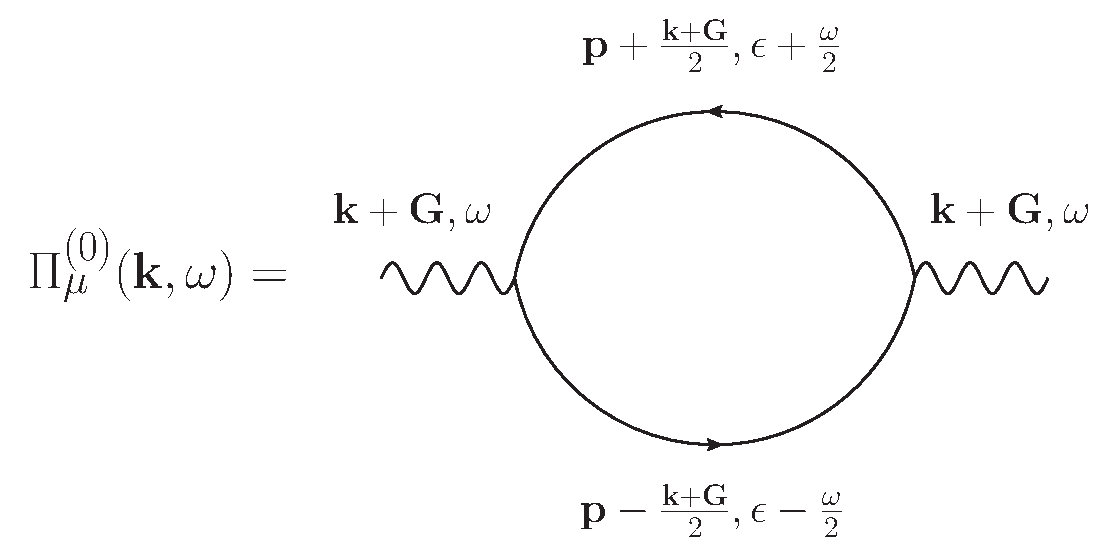
\includegraphics[width=0.5\textwidth]{bubble_diagram.eps}
	\caption{caption}
	\label{fig:bubble diagram}
\end{figure}
%
The bubble diagram is the lowest order of the full polarization operator.
In the following this diagram is computed in detail.
The first order of the polarization bubble is given by
%
\begin{align}
	\Pi_{\mu}^{(0)}(\vb{k}, \omega) = 
		i 
		\sum\limits_{\vb{P}}
		\int\limits_{|p| \leq |p_{\mt{F}}} \frac{\dd[2]{\vb{p}}}{(2\pi)^{2}} 
		\int\limits_{-\infty}^{\infty} \frac{\dd{\epsilon}}{2\pi}\,
		\mathcal{G}_{\mt{a}}^{(0)}(\vb{p}+\frac{\vb{k}}{2}, \epsilon+\frac{\omega}{2})
		\mathcal{G}_{\mt{b}}^{(0)}(\vb{p}-\frac{\vb{k}}{2}, \epsilon-\frac{\omega}{2}).
\end{align}
%
Here the outer momentum and frequency is shfited to symmetrizie the argument of both fermionic Green functions.
The Green function is given by
%
\begin{align}
	 \mathcal{G}_{\alpha}^{(0)}(\vb{k},\omega) := \green{\Psi_{\alpha}}{\Psi_{\alpha}^{\dag}}_{\omega} = \sum\limits_{\vb{G}} \frac{1}{\omega - \epsilon_{\alpha}(\vb{k}+\vb{G})}, 
	 \label{appeq:free electron propagator}
\end{align}
%
where the species of the corresponding fermions is indicated with the index $\alpha = \mt{a},\mt{b}$.
First of all, the dispersion relation of the fermions is investigated.
Spin fluctuations interact only with fermions near the Fermi surface.
Under this condition, the dispersion relation of the fermions of species a is expanded.
%
\begin{align}
	\epsilon_{\mt{a}}(\vb{p} + \frac{\vb{k} + \vb{G}}{2}) &= 
		\frac{\big(p_{x} + \frac{k_{x} + G_{x}}{2}\big)^{2}}{2m_{1}} 
		+ 
		\frac{\big(p_{y} + \frac{k_{y} + G_{y}}{2}\big)^{2}}{2m_{2}} 
		\notag \\ 
	\Leftrightarrow\ \epsilon_{\mt{a}}(\vb{p} + \frac{\vb{k} + \vb{G}}{2}) &=
		\frac{p_{x}^{2}}{2m_{1}} + \frac{1}{2} \frac{p_{x}}{m_{1}}(k_{x}+G_{x}) + \frac{(k_{x}+G_{x})^{2}}{8m_{1}}
		\notag \\ &+
		\frac{p_{y}^{2}}{2m_{2}} + \frac{1}{2} \frac{p_{y}}{m_{2}}(k_{y}+G_{y}) + \frac{(k_{y}+G_{y})^{2}}{8m_{2}}
		\notag \\
	\Leftrightarrow\ \epsilon_{\mt{a}}(\vb{p} + \frac{\vb{k} + \vb{G}}{2}) &\approx
		\xi_{\mt{a}} + \frac{1}{2} \vb{v}_{\mt{a,F}}(\vb{k} + \vb{G}) + \mu
\end{align} 
%
where the quadratic term with respect to $\vb{k}$ is neglected and $\xi_{\mt{a}}$ is the dispersion denoted in equation \eqref{eq:dispersion relations}.
Moreover, the velocity $\vb{v}_{a}$ of the fermion of species a is introduced.
Since only fermions near the Fermi surface are considered the velocity is assumed to be the Fermi velocity.
The same procudure is valid for the fermions of species b.
Finally, the normalized momentum vector $\vb{n} = \frac{\vb{p}}{|\vb{p}|}$ is introduced.
The Fermi velocity of fermions of species a is then given by $\vb{v}_{\mt{a,F}} = v_{\mt{a,F}} \vb{n}$ and equally for b.
The scalar product between the normalized momentum vector $\vb{n}$ and the bosonic spin density wave vector $\vb{k} + \vb{G}$ is rewriten as the magnitude multiplied with $\cos(\vartheta)$, where $\vartheta$ is the angle between both.

In the investigated model, the points of interaction between the fermions caused by spin fluctuations are hot-spots (see chapter \ref{ch:spin fermion model}).
This are certain points on the Fermi surface seperated by the momentum vector $\vb{Q}$.
The energy and the magnitudes of the Fermi velocities are equal on these points connected wby $\vb{Q}$.
%
\begin{align}
	\xi := \xi_{\mt{a}} = \xi_{\mt{b}} \qquad v_{\mt{F}} := v_{\mt{a,F}} = v_{\mt{b,F}}
\end{align}
%
The direction of the velocities have to be unequal
Otherwise, the angle $\vartheta$ is $0$ or $\pi$ and the imaginary part of $\Pi_{\mu}$ is zero.
Using these conversions and assumptions, the polarization operator is given by
%
\begin{align}
	\Pi_{\mu}^{(0)}(\vb{k}, \omega) &= 
		i \nu_{\mt{F}}
		\int\limits_{0}^{\pi} \dd{\vartheta}
		\int\limits_{\xi \leq \xi_{\mt{F}}} \dd{\xi}
		\int\limits_{-\infty}^{\infty} \frac{\dd{\epsilon}}{2\pi}
		\notag \\ &\times
		\frac{1}{\epsilon + \frac{\omega}{2} - \xi - \frac{1}{2} v_{\mt{F}} |\vb{k} + \vb{G}| \cos(\vartheta) + i \eta \sign(\epsilon + \frac{\omega}{2})}
		\notag \\ &\times
		\frac{1}{\epsilon - \frac{\omega}{2} - \xi + \frac{1}{2} v_{\mt{F}} |\vb{k} + \vb{G}| \cos(\vartheta) + i \eta \sign(\epsilon - \frac{\omega}{2})}.
	\label{appeq:pol operator before epsilon integration}
\end{align}
%
Here, the two dimensional momentum integral is firstly transformed in plane polar coordinates and then the $k$-integral is transformed into an energy integral over the density of states.
The density of states is approximated with the value of the density of states at the Fermi surface, $\nu_{\mt{F}} := \nu(\xi_{\mt{F}})$, since only fermions near the Fermi surface are considered.
The energy integral is limited by the Fermi energy $\xi_{\mt{F}}$.

The further treatment is started by computing the frequency integral.
The integral over $\epsilon$ is transformed into a complex contour integral, where the contour $\Gamma$ is chosen in two different ways.
According to the singularities of the integrand the countour is closed in the upper or lower half plane using a semicircle with radius infinity.
In both cases the contribution of the semicircle is zero, since the integrand is proportional to $\flatfrac{1}{\epsilon}$.
The equality between the integral along the real axis and the complex contour integral is ensured due to the non-contributing of the semicircle.
The investigated integrand has two singularities at
%
\begin{align}
	\epsilon_{1} := \xi - \frac{1}{2}\big(\omega - v_{\mt{F}} |\vb{k} + \vb{G}| \cos(\vartheta)\big) 
	\qq{and}
	\epsilon_{2} := \xi + \frac{1}{2}\big(\omega - v_{\mt{F}} |\vb{k} + \vb{G}| \cos(\vartheta)\big),
\end{align}
%
where both singularities are of first order.
The poles are located in the upper or lower plane, according to the signum function in the denominator.
In total four different constitutions are possible.
On the one hand, both singularities can be located in the lower or upper complex plane, which yield in both cases zero.
On the other hand, one pole is sited in the upper plane, while the other one is sited in the lower plane, or vice versa, where both yield the same contribution
%
\paragraph{1. case:} $\sign(\epsilon + \frac{\omega}{2}) = \sign(\epsilon - \frac{\omega}{2})$\\
%
Both singularities are located in the upper or in the lower complex half plane.
The contour is therefore closed in the upper or lower plane, respectivily, enclosing both poles .
In the first case the winding number is $1$, since the pole is enclosed counterclockwise.
Accordingly, the winding number is $-1$ in the second case.
%
\begin{align}
	&\mt{I}_{\omega}^{\mt{e}} := i \oint_{\Gamma} \frac{\dd{\omega}}{2\pi i}\, \frac{1}{\omega - \omega_{1} \mp i\eta} \cdot \frac{1}{\omega - \omega_{2} \mp i\eta}
	\notag \\
	\Leftrightarrow\ &\mt{I}_{\omega}^{\mt{e}} = \pm i \bigg[ \frac{1}{\omega_{2} - \omega_{1}} + \frac{1}{\omega_{1} - \omega_{2}}\bigg] = 0,
\end{align}
%
where the index "e" stands for even and means, that both poles are located in the same half plane.
%
\paragraph{2. case:} $\sign(\epsilon + \frac{\omega}{2}) \neq \sign(\epsilon - \frac{\omega}{2})$\\
%
The singularities are sited in different complex half planes, one in the upper and accordingly the other in the lower half plane.
It is arbitrary in which half plane the contour is closed as long as one pole is enclosed.
In the following computation the contour is closed in the upper half plane.
%
\begin{align}
	&\mt{I}_{\omega}^{\mt{o}} := i \oint_{\Gamma} \frac{\dd{\omega}}{2\pi i}\, \frac{1}{\omega - \omega_{1} \mp i\eta} \cdot \frac{1}{\omega - \omega_{2} \pm i\eta}
	\notag \\
	\Leftrightarrow\ &\mt{I}_{\omega}^{\mt{o}} = \frac{\pm i}{\omega_{2} - \omega_{1} \pm i\eta}
\end{align}
%
where the index "o" stands for odd and mean, that both poles are located in opposite half planes.

After inserting both expressions for the singularities $\omega_{1}$ and $\omega_{2}$, the intergand is independent with respect to $\xi$
The signum functions in \eqref{appeq:pol operator before epsilon integration} is equivalent to the signum functions $\sign(\xi \pm \frac{1}{2} v_{\mt{F}} |\vb{k} + \vb{G}| \cos(\vartheta))$ in energy representation.
The energy $\xi$ is dropped, since the integrand is independent of $\xi$, and the constant positive factors are neglectable. 
Then, the signum function is expressed as $\sign[|\vb{k} + \vb{G}| \cos(\vartheta))$.
Finally, the integrals limits are set to $\pm \frac{1}{2} v_{\mt{F}} |\vb{k} + \vb{G}| \cos(\vartheta)$, which follows directly from the localization of both poles.
$\omega_{1}$ is assumed to be in the lower half plane, while $\omega_{2}$ is then assumed in the opposite one.
This implies that $\epsilon + \frac{\omega}{2} > 0$ and $\epsilon - \frac{\omega}{2} < 0$, respectivily.
Transforming into energy representation the obtained expression yield the definition interval of $\xi$.
The polarization operator is therefore given by
%
\begin{align}
	\Pi_{\mu}^{(0)}(\vb{k}, \omega) &= 
		i \nu_{\mt{F}}
		\int\limits_{0}^{\pi} \dd{\vartheta} 
		\int\limits_{-\xi_{0}}^{\xi_{0}} \dd{\xi}
		\frac{i \sign(|\vb{k} + \vb{G}| \cos(\vartheta))}{\omega - v_{\mt{F}} |\vb{k} + \vb{G}| \cos(\vartheta) + i\eta \sign(|\vb{k} + \vb{G}| \cos(\vartheta))},
\end{align}
%
where the abbreviation $\xi_{0} = \flatfrac{v_{\mt{F}}|\vb{k}+\vb{G}|\cos(\vartheta)}{2}$ is introduced.
The integration over $\xi$ yields the factor $v_{\mt{F}}|\vb{k}+\vb{G}|\cos(\vartheta)$.
Subsequently the signum function is reexpressed in frequency representation corresponding to $\sign(\omega)$.
Since our interest is attracted to damping of the spin fluctuations, the imaginary part of the polarization operator is taken:
%
\begin{align}
	\Im{\Pi_{\mu}^{(0)}(\vb{k}, \omega)} &= 
		\nu_{\mt{F}} \pi
		\int\limits_{0}^{\pi} \dd{\vartheta}
		v_{\mt{F}} |\vb{k}+\vb{G}| \cos(\vartheta) \delta(\omega - v_{\mt{F}} |\vb{k} + \vb{G}| \cos(\vartheta)).
	\label{appeq:imaginary part of pol operator before theta integration}
\end{align}
%
Here the formula $\frac{1}{x \pm i\eta} = \PV{\frac{1}{x}} \mp i \pi \delta(x)$ is used.
The obtained $\delta$-distribution has a function $g(\vartheta)$  as argument.
Using formula
%
\begin{align}
	\delta(g(x)) = \sum\limits_{i=1} \frac{\delta(x-x_{0,i})}{|g'(x_{0,i})|},
\end{align}
%
the $\delta$-distribution is rewriten as a sum over $\delta$-distributions with the zeros of $g(\theta)$ as argument.
In the above formula, the sum runs over all zeros of $g(x)$, which are denoted as $x_{0,i}$.
The derivative with respect to $x$ is labeled with a prime at $g$ and is evaluated at the corresponding zero $x_{0,i}$.

In our observed case, the argument of $\delta(g(\vartheta))$ contains only one zero at $\vartheta_{0} = \cos[-1](\flatfrac{\omega}{(v_{\mt{F}} |\vb{k} + \vb{G}|)})$ inside the integral boundaries.
The $\delta$-distribution is rewriten as:
%
\begin{align}
	&\delta(\omega - v_{\mt{F}} |\vb{k} + \vb{G}| \cos(\vartheta)) = \Big(v_{\mt{F}} |\vb{k} + \vb{G}| \cdot |\sin(\vartheta_{0})|\Big)^{-1} \delta(\vartheta - \vartheta_{0})
	\notag \\
	\Rightarrow\ &\delta(\omega - v_{\mt{F}} |\vb{k} + \vb{G}| \cos(\vartheta)) \approx \Big(v_{\mt{F}} |\vb{k} + \vb{G}|\Big)^{-1} \delta(\vartheta - \vartheta_{0}).
\end{align}
%
In the second line the limit of small frequancies $\omega$ is taken, which is valid in our observed low-energy theory in the spin fermion model.
The integration over $\vartheta$ is now performed and the imaginary part of the polarization operator is given by
%
\begin{align}
	\Im{\Pi_{\mu}^{(0)}(\vb{k}, \omega)} &= \frac{\nu_{\mt{F}} \pi}{v_{\mt{F}} |\vb{k} + \vb{G}|} \cdot \omega = \gamma \omega,	 
\end{align}
%
where the damping parameter $\gamma$ is introduced.
As above demonstrated, the damped spin density propagator is determined by the Dyson equation \eqref{appeq:Dyson equation}.
The polarization operator is reperated into real and imaginary part.
Inserting the free spin density propagator and the obtained result for $\Im{\Pi_{\mu}}$, the damped spin density popagator is obtained to
%
\begin{align}
	\mathcal{D}_{\mu}(\vb{k}, \omega) = \sum\limits_{\vb{G}} \frac{1}{(\vb{k}+\vb{G})^{2} + r - (\flatfrac{\omega}{v_{\mt{S}}})^{-2} - i \gamma \omega}
	\label{appeq:damped spin density propagator with real omega}
\end{align}
%
where the abbreviation $r = r_{0} - \Re{\Pi_{\mu}(\vb{k}, \omega)}$ is used.
In the vicinity of the quantum critical point the real part of $\Pi_{\mu}$ is canceled by $r_{0}$, since the correlations length is divergent and $r=\xi^{-2}$
In low-energy theory, the $\omega^{2}$-term is further neglectable.
%
%
\section{Transformation into Matsubara Frequency Space}
\label{appsec:transformation into Matsubara frequency space}
%
%
The spin density wave propagator, obtained in the previous section, is a complex function of the real quantity $\omega$.
In the following, the quantity $\omega$ is transformed into an imaginary quantity $i\omega_{n}$, known as Matsubara frequancies.
The real and imaginary part of the propagator $\mathcal{D}_{\mu}(\vb{k}, i\omega_{n})$ with respect to Matsubara frequencies is evaluated using the Kramers-Kronig relations \cite{Schwabl}.
The propagator in \eqref{appeq:damped spin density propagator with real omega} is seperated into real and imaginary part, extending with the complex conjugated denominater.
%
\begin{align}
	\mathcal{D}_{\mu}(\vb{k}, \omega) = \sum\limits_{\vb{G}} \bigg[\frac{(\vb{k}+\vb{G})^{2}}{(\vb{k}+\vb{G})^{4} + (\gamma\omega)^{2}} + i \frac{\gamma \omega}{(\vb{k}+\vb{G})^{4} + (\gamma\omega)^{2}}\bigg],
	\label{appeq:real and imaginary part of D}
\end{align}
%
where $r$ and $\xi$ is set to zero.
For the following treatment it is usefull to investigate the symmetries of the real and imaginary part.
The real part is a symmetric function and the imaginary part is an antiysmmetric funtion, with respect to $\omega$.
The imarginary part of $\mathcal{D}_{\mu}(\vb{k}, i\omega_{n})$ is evaluated to zero, since its defined as the integral over the real part of $\mathcal{D}_{\mu}(\vb{k}, \omega)$ divided by $\omega$.
The integrand is therefore an odd function and the integral over all frequencies $\omega$ is zero.
In Matsubara frequency space, the damped propagator is given by its real part.
%
\begin{align}
	\mathcal{D}_{\mu}(\vb{k}, i\omega_{n}) = \Re{\mathcal{D}_{\mu}(\vb{k}, i\omega_{n})} = \frac{1}{\pi}\: \PV{\int\limits_{-\infty}^{\infty} \dd{\omega} \frac{\Im{\mathcal{D}_{\mu}(\vb{k}, \omega)}}{\omega - i\omega_{n}}}
\end{align}
%
where $\PV$ represents that the integrals is evaluated using the principal value.
The integral is speperated into two parts. 
In the first one $\omega$ is substituted by $-\omega$ and the antismmetry of $\Im{\mathcal{D}_{\mu}(\vb{k}, \omega)}$ is utilizied.
%
\begin{align}
	&\mathcal{D}_{\mu}(\vb{k}, i\omega_{n}) = \frac{1}{\pi} \int\limits_{0}^{\infty} \dd{\omega} \Im{\mathcal{D}_{\mu}(\vb{k}, \omega)} \Bigg[
		\frac{1}{\omega + i\omega_{n}}
		+
		\frac{1}{\omega - i\omega_{n}}
	\Bigg]
	\notag \\
	\Leftrightarrow\ &\mathcal{D}_{\mu}(\vb{k}, i\omega_{n}) = 
		\frac{2}{\pi} \sum\limits_{\vb{G}} \int\limits_{0}^{\infty} \dd{\omega} 
		\frac{\gamma \omega}{(\vb{k}+\vb{G})^{4} + (\gamma\omega)^{2}} \cdot
		\frac{\omega}{\omega^{2} + \omega_{n}^{2}}
	\notag \\
	\Leftrightarrow\ &\mathcal{D}_{\mu}(\vb{k}, i\omega_{n}) = 
		\sum\limits_{\vb{G}} \frac{1}{(\vb{k}+\vb{G})^{2} + \gamma|\omega_{n}|}
	\label{eq: damped propagator Matsubara representation}
\end{align}
%
In the last step the integral formula
%
\begin{align}
	\int\limits_{0}^{\infty} \dd{x} \frac{x}{a^{2} + x^{2}} \cdot \frac{x}{y^{2} + x^{2}} = \frac{\pi}{2} \frac{1}{a + |y|}
\end{align}
%
is used, which can be shown by transforming into a complex contour integral.

















%The spin fermion model considers an interaction between electrons on different Fermi surfaces, where the interaction is originated by spin density waves.
%On that reason the propagation of the spin density waves is damped.
%The damping should be considered in the propagator via doing pertubation theory.

%Because the damping is originated by the interaction between electrons the free electron propagator is also needed in the following calculation.
%The propagator can be calculated in the same way as the  one for free spin density waves.
%This handwork shouldn't be done here explicitly.
%The free electron propagator is given by
%
%\begin{align}
%	 \mathcal{G}_{\alpha}^{(0)}(\vb{k},\omega) := \green{\Psi_{\alpha}}{\Psi_{\alpha}^{\dag}}_{\omega} = \sum\limits_{\vb{G}} \frac{1}{\omega - \epsilon_{\alpha}(\vb{k}+\vb{G})}, 
%	 \label{eq: free electron propagator}
%\end{align}
%
%where $\alpha = \mt{a,b}$ denotes the Fermi surface of the respective electrons.
%The damped spin density wave propagator is computed using the usually method of pertubation theory in quantum field theory.



 %done
%
%
%
\chapter{Time Derivative of Momentum P and Current J}
\label{appch:time derivative P and J}
%
%
%
The time derivative of the momentum and current operator are designated for the case of non-pertubation and pertubation in chapter \ref{ch:spin fermion model}.
In this appendix, the computation is outlined of them.
Our further approach is to compute Hamiltonian, momentum and current operator, using the energy-momentum-tensor and current-tensor \cite{Iliev}.
The time derivative of momentum and current is then calculated, using the Heisenberg equation of motion.
In the end, umklapp scattering is observed and the effect to momentum and current are discussed.

Our starting point is the Lagrangian $\mathcal{L} = \mathcal{L}_{\Psi} + \mathcal{L}_{\Phi} + \mathcal{L}_{\Psi\Phi}$, as suggested in \cite{Patel&Sachdev} of the spin-fermion-model.
In Matsubara time $\tau = it$, the single Lagrangians are given by
%
\begin{align}
	\mathcal{L}_{\Psi} = 
		\vb{\Psi}^{\dag}(\vb{x},\tau)
		\twoTwoMatrix{\sigma_{0} (\partial_{\tau}+\mu_{0}+\xi_{a})}{0}{0}{\sigma_{0} (\partial_{\tau}+\mu_{0}+\xi_{b})}
		\vb{\Psi}(\vb{x},\tau)
\end{align}
%
\begin{align}
	\mathcal{L}_{\Phi} &= 
		\frac{1}{2} \big[\partial_{i}\Phi_{\mu}(\vb{x},\tau)\big] \big[\partial_{i}\Phi_{\mu}(\vb{x},\tau)\big] 
		+ 
		\frac{\epsilon}{2} \big[\partial_{\tau}\Phi_{\mu}(\vb{x},\tau)\big] \big[\partial_{\tau}\Phi_{\mu}(\vb{x},\tau)\big] 
		\notag \\&+
		\frac{u}{6} \Big[\Phi_{\mu}(\vb{x},\tau) \Phi_{\mu}(\vb{x},\tau) + \frac{3}{g}\Big]^{2}
\end{align}
%
\begin{align}
	\mathcal{L}_{\Psi\Phi} =
		\lambda\Phi_{\mu}(\vb{x},\tau) \Big[\Psi_{\mt{a}}^{\dag}(\vb{x},\tau) \sigma_{\mu} \Psi_{\mt{b}}(\vb{x},\tau) + \Psi_{\mt{b}}^{\dag}(\vb{x},\tau) \sigma_{\mu} \Psi_{\mt{a}}(\vb{x},\tau)\Big]
\end{align}
%
Here $\vb{\Psi} = (\Psi_{\mt{a}}, \Psi_{\mt{b}})$ is a vector containing the two-component spinors $\Psi_{\mt{a}}$, $\Psi_{\mt{b}}$.
$\Phi_{\mu}$ is the three component bosnoic field operator and describes the spin fluctuations in the spin-fermion-model.
Since the spin fluctuations arise at the phase transition, $\Phi_{\mu}$ is order parameter as well.
The chemical potential is denoted with $\mu_{0}$ and the Pauli matrix are labeled with $\sigma_{0}$ and $\sigma_{\mu}$.
The abbreviation $\epsilon = v_{\mt{S}}^{-2}$ is introduced, where $v_{\mt{S}}$ is the spin velocity.
In the Lagrangian $\mathcal{L}_{\Phi}$, the term in the second line is neglectable in the low-energy theory of the spin fermion model.
The anisotropic parabolical dispersion relations $\xi_{\mt{a}}$ and $\xi_{\mt{b}}$ are given by 
%
\begin{align}
	\xi_{\mt{a}} = \frac{\partial_{x}^{2}}{2m_{1}} + \frac{\partial_{y}^{2}}{2m_{2}} \qquad \xi_{\mt{b}} = \frac{\partial_{x}^{2}}{2m_{2}} + \frac{\partial_{y}^{2}}{2m_{1}}
\end{align}
%
The Hamiltonian for umklapp scattering is assumed to be 
%
\begin{align}
	\mathcal{H}_{\mt{umklapp}}= \mt{J}(\vb{R}) \Phi_{\mu}(\vb{x},\tau) \Phi_{\mu}(\vb{x},\tau)
\end{align}
%
where $\mt{J}(\vb{R})$ is a coupling parameter and $\vb{R}$ is a lattice vector.
In a first step, the Hamiltonian for the unpertubated spin-fermion-model is calulated using the energy-momentum-tensor and current-tensor \cite{Iliev}.
%
\begin{align}
	\mathcal{T}_{\mu\nu} = 
		\frac{1}{2} \sum\limits_{\zeta_{n}} \bigg[ 
		\Big(\frac{\partial\mathcal{L}}{\partial(\partial_{\mu}\zeta_{n})}\Big) (\partial_{\nu}\zeta_{n}) 
		+
		(\partial_{\nu}\zeta_{n})^{\dag} \Big(\frac{\partial\mathcal{L}}{\partial(\partial_{\mu}\zeta_{n})}\Big)^{\dag}
		\bigg]
		-\eta_{\mu\nu}\mathcal{L}
\end{align}
%
%
\begin{align}
	\mathcal{J}_{\mu} = -i \sum\limits_{\{\zeta_{n}\}} \epsilon(\zeta_{n}) \bigg[
		\Big(\frac{\partial\mathcal{L}}{\partial(\partial_{\mu}\zeta_{n})}\Big) \zeta_{n}
		-
		\zeta_{n}^{\dag} \Big(\frac{\partial\mathcal{L}}{\partial(\partial_{\mu}\zeta_{n})}\Big)^{\dag}
		\bigg],
\end{align}
%
Here, $\zeta_{n}$ is the set of all contributing operator fields, which is in our case $\{\Psi_{\mt{a}},\Psi_{\mt{b}}, \Phi_{\mu}\}$.
The function $\epsilon(\zeta_{n})$ attains the values 0 of 1 in the case of real or complex fields, respectively.
$\eta_{\mu\nu}$ is the Minkowski metric, where the definition $(1,-1,-1,-1)$ is used here.
In chapter \ref{ch:spin fermion model}, the concept of hot spots is introduced.
Fermions on different Fermi surfaces interact via spin fluctations, described by $\Phi_{\mu}$.
The bosonic field operators are supposed to be real quantities, since the interaction is assumed to be on the hot spots and not in a vicinity regime around them.
Furthermore, the spatial derivative in $\mathcal{L}_{\Psi}$ is rewriten. using relation $\Psi^{\dag} (\partial_{i}^{2} \Psi) = -(\partial_{i} \Psi^{\dag}) (\partial_{i} \Psi)$.
This relation is evaluated, integrating the left hand side by parts.

The (00)-component of the energy-momnetum-tensor represents the Hamiltonian of a system.
This quantity is computed in the following.
%
\begin{align}
	\mathcal{H} &= 
		\frac{1}{2} \sum\limits_{\zeta_{n}} \bigg[
		\Big(\frac{\partial\mathcal{L}}{\partial(\partial_{\tau}\zeta_{n})}\Big) (\partial_{\tau}\zeta_{n}) 
		-
		(\partial_{\tau}\zeta_{n}^{\dag}) \Big(\frac{\partial\mathcal{L}}{\partial(\partial_{\tau}\zeta_{n})}\Big)^{\dag}
		\bigg]
		-
		\mathcal{L}
		\notag \\
	\Leftrightarrow\ \mathcal{H} &= 
		\Psi_{\mt{a}}^{\dag} (\partial_{\tau}\Psi_{\mt{a}}) 
		+
		\Psi_{\mt{b}}^{\dag} (\partial_{\tau}\Psi_{\mt{b}}) 
		+
		\epsilon  (\partial_{\tau} \Phi_{\mu}) (\partial_{\tau} \Phi_{\mu}) 
		-
		\mathcal{L}
	\notag \\
	\Leftrightarrow\ \mathcal{H} &= 
		-
		\Psi_{\mt{a}}^{\dag}(\vb{x},\tau) \big(\frac{\partial_{x}^{2}}{2m_{1}} + \frac{\partial_{y}^{2}}{2m_{2}} + \mu_{0}\big) \Psi_{\mt{a}}(\vb{x},\tau)
		\notag \\&
		- 
		\Psi_{\mt{b}}^{\dag}(\vb{x},\tau) \big(\frac{\partial_{x}^{2}}{2m_{2}} + \frac{\partial_{y}^{2}}{2m_{1}} + \mu_{0}\big) \Psi_{\mt{b}}(\vb{x},\tau)
		\notag \\&
		- 
		\frac{1}{2} \big(\partial_{i} \Phi_{\mu}(\vb{x},\tau)\big) \big(\partial_{i} \Phi_{\mu}(\vb{x},\tau)\big)
		+ 
		\frac{1}{2\epsilon} \pi_{\mu}(\vb{x},\tau) \pi_{\mu}(\vb{x},\tau)
		\notag \\&
		-	
		\lambda \Phi_{\mu}(\vb{x},\tau) \big(\Psi_{\mt{a}}^{\dag}(\vb{x},\tau) \sigma_{\mu} \Psi_{\mt{b}}(\vb{x},\tau) + \Psi_{\mt{b}}^{\dag}(\vb{x},\tau) \sigma_{\mu} \Psi_{\mt{a}}(\vb{x},\tau)\big)
\end{align}
%
Here, the usual time derivative is transformed into the Matsubara time, using $\partial_{t} = -i\partial_{\tau}$.
The Hermitain of the $\tau$-derivative is given by $(\partial_{\tau})^{\dag} = -\partial_{\tau}$, which is also used.
The canonical momentum of $\Phi_{\mu}$, given by $\pi_{\mu}(\vb{x},\tau) = \epsilon \partial_{\tau} \Phi_{\mu}(\vb{x},\tau)$, is used in the last step.
The $\mathcal{T}_{0j}$-component is identified with the $j$-component of the momentum operator, which is calculated as next.
%
\begin{align}
	\mathcal{P}_{j} &= 
		\frac{-i}{2} \sum\limits_{\zeta_{n}} \bigg[ 
		\Big(\frac{\partial\mathcal{L}}{\partial(\partial_{\tau}\zeta_{n})}\Big) (\partial_{j}\zeta_{n}) 
		+
		(\partial_{j}\zeta_{n})^{\dag} \Big(\frac{\partial\mathcal{L}}{\partial(\partial_{\tau}\zeta_{n})}\Big)^{\dag}
		\bigg]
		-
		\eta_{0j}\mathcal{L}
		\notag \\
	\Leftrightarrow\ \mathcal{P}_{j} &= 
		\frac{-i}{2} \bigg[
			\Psi_{\mt{a}}^{\dag}(\vb{x},\tau) \big(\partial_{j} \Psi_{\mt{a}}(\vb{x},\tau)\big)
			- 
			\big(\partial_{j} \Psi_{\mt{a}}^{\dag}(\vb{x},\tau)\big) \Psi_{\mt{a}}(\vb{x},\tau)
			\notag \\&
			+
			\Psi_{\mt{b}}^{\dag}(\vb{x},\tau) \big(\partial_{j} \Psi_{\mt{b}}(\vb{x},\tau)\big)
			- 
			\big(\partial_{j} \Psi_{\mt{b}}^{\dag}(\vb{x},\tau)\big) \Psi_{\mt{b}}(\vb{x},\tau)
		\bigg]
		- 
		i\pi_{\mu}(\vb{x},\tau)) \big(\partial_{j} \Phi_{\mu}(\vb{x},\tau)\big)
	\notag \\
	\Rightarrow\ \vb{\mathcal{P}} &= 
		\frac{-i}{2} \bigg[
			\vb{\Psi}^{\dag}(\vb{x},\tau) \big(\nabla \vb{\Psi}(\vb{x},\tau)\big)
			- 
			\big(\nabla \vb{\Psi}^{\dag}(\vb{x},\tau)\big) \vb{\Psi}(\vb{x},\tau)
		\bigg]
		-
		i \pi_{\mu}(\vb{x},\tau) \big(\nabla \Phi_{\mu}(\vb{x},\tau)\big)
\end{align}
%
The Hermitian of the $\tau$-derivative and the canonical momentum is again used at this computation.
The two-component vector $\vb{\Psi}$ is inserted to write the vector components as vector.
Now, the $x$-component of the current is caluclated.
%
\begin{align}
	\mathcal{J}_{x} &= 
		-i \sum\limits_{\zeta_{n}} \epsilon(\zeta_{n}) \bigg[
			\Big(\frac{\partial\mathcal{L}}{\partial(\partial_{x}\zeta_{n})}\Big) \zeta_{n}
			-
			\zeta_{n}^{\dag} \Big(\frac{\partial\mathcal{L}}{\partial(\partial_{x}\zeta_{n})}\Big)^{\dag}
		\bigg]
	\notag \\
	\Leftrightarrow\ \mathcal{J}_{x} &=
		\frac{-i}{2} \bigg[
		\frac{1}{m_{1}} \Big[
			\big(\partial_{x} \Psi_{\mt{a}}^{\dag}(\vb{x},\tau)\big) \Psi_{\mt{a}}(\vb{x},\tau)
			-
			\Psi_{\mt{a}}^{\dag}(\vb{x},\tau) \big(\partial_{x} \Psi_{\mt{a}}(\vb{x},\tau)\big)
		\Big]
		\notag \\&
		+
		\frac{1}{m_{2}} \Big[
			\big(\partial_{x} \Psi_{\mt{b}}^{\dag}(\vb{x},\tau)\big) \Psi_{\mt{b}}(\vb{x},\tau)
			-
			\Psi_{\mt{b}}^{\dag}(\vb{x},\tau) \big(\partial_{x} \Psi_{\mt{b}}(\vb{x},\tau)\big)
		\Big]
		\bigg]
\end{align}
%
The $x$-component of the current is compted analogical, where an interchange of the mass $(m_1 \leftrightarrow m_2)$ is the only difference. 
These three quantities are now transformed into momentum space, since all of them contains spatial derivatives.
This is obstructive in the later caluclation of the time derivative of P and J, since commutator relations of fermionic and bosonic fields are therefore used.
%
\begin{align}
	\mt{H} &= 
	 	\int_{\vb{k}}
	 	\Bigg[ \sum\limits_{\alpha} \epsilon_{\alpha}(\vb{k}) \Psi_{\alpha}^{\dag}(\vb{k},\tau) \Psi_{\alpha}(\vb{k},\tau)
		-
		\frac{\vb{k}^{2}}{2} \Phi_{\mu}(\vb{k},\tau) \Phi_{\mu}(-\vb{k},\tau)
		+
		\frac{1}{2\epsilon} \pi_{\mu}(\vb{k},\tau) \pi_{\mu}(-\vb{k},\tau)
		\notag \\ &
		-
		\lambda \int_{\vb{q}} \Phi_{\mu}(\vb{k}-\vb{q},\tau)
		\bigg[
			\Psi_{\mt{a}}^{\dag}(\vb{k},\tau) \sigma_{\mu} \Psi_{\mt{b}}(\vb{q},\tau)
			+
			\Psi_{\mt{b}}^{\dag}(\vb{k},\tau) \sigma_{\mu} \Psi_{\mt{a}}(\vb{q},\tau)
		\bigg]
		\Bigg]
\end{align}
%
%
\begin{align}
	\mt{P}_{j} &= \int_{\vb{k}}
		k_{j} \Bigg[ \sum\limits_{\alpha} \Psi_{\alpha}^{\dag}(\vb{k},\tau) \Psi_{\alpha}(\vb{k},\tau)
	 	-
	 	\pi_{\mu}(\vb{k},\tau)
	 	\Phi_{\mu}(-\vb{k},\tau)
	\Bigg]
\end{align}
%
%
\begin{align}
	\mt{J}_{x} &= - \int_{\vb{k}} \Bigg[
		\frac{k_{x}}{m_{1}}
		\Psi_{\mt{a}}^{\dag}(\vb{k},\tau)
		\Psi_{\mt{a}}(\vb{k},\tau)
		+
		\frac{k_{x}}{m_{2}}
		\Psi_{\mt{b}}^{\dag}(\vb{k},\tau)
		\Psi_{\mt{b}}(\vb{k},\tau)
	\Bigg]
\end{align}
%
The sum over $\alpha$ summarizes over the two species of fermions a and b.
Their dispersion relations are given by $\epsilon_{\mt{a}}(\vb{k}) = \frac{k_{x}^{2}}{2m_{1}} + \frac{k_{y}^{2}}{2m_{2}} - \mu_{0}$ und $\epsilon_{\mt{b}}(\vb{k}) = \frac{k_{x}^{2}}{2m_{2}} + \frac{k_{y}^{2}}{2m_{1}} - \mu_{0}$ in momentum space.
All integrals are extended over the first Brillouin zone.

Now, the time derivative of momentum P and current J is computed.
The Heisenberg equation of motion is the usual way to calculate the derivative of an operator in quantum mechanics.
The simplicity of this method is, that only the commutator between the Hamiltonian and the observed operator has to be computed.
For the further approach, the commutator relations for bosonic and fermionic fields are required.
Beside these two ones, all other commutator relations yield zero.
%
\begin{align}
	\acomm{\Psi_{\mt{\alpha}}(\vb{k},\tau)}{\Psi_{\mt{\beta}}^{\dag}(\vb{p},\tau)} &= (2\pi)^{2} \delta_{\mt{\alpha}\mt{\beta}} \delta(\vb{p}-\vb{k})
	\\
	\comm{\Phi_{\mu}(\vb{k},\tau)}{\pi_{\lambda}(\vb{p},\tau)} &= (2\pi)^{2} \delta_{\mu\lambda} \delta(\vb{p}+\vb{k})
\end{align}
%
At first the commutator between the Hamiltonian H and the $x$-component of P is computed.
All integrals are extended over the first Brillouin zone, while the sums over greek letters runs over the fermionic species a and b.
The condition $\alpha \neq \beta$ means that in this case both greek latters has to be different.
The commutator has to be transformed into component representation, if Pauli matricies $\sigma_{\mu}$ connects to fermionic field operators.
The above commutator relations are also valid in this representation.
%
\begin{align}
	\comm{\mt{H}}{\mt{P}_{x}} &= 
		\int_{\vb{k}} \int_{\vb{p}}
		p_{x}
		\sum\limits_{\alpha,\beta} 
		\epsilon_{\alpha}(\vb{k})
		\comm{\Psi_{\alpha}^{\dag}(\vb{k},\tau) \Psi_{\alpha}(\vb{k},\tau)}{\Psi_{\beta}^{\dag}(\vb{k},\tau) \Psi_{\beta}(\vb{k},\tau)}
		\notag \\&
		+
		\int_{\vb{k}} \int_{\vb{p}}
		p_{x}
		\bigg[
			\frac{k^{2}}{2}
			\comm{\Phi_{\mu}(\vb{k},\tau) \Phi_{\mu}(-\vb{k},\tau)}{\pi_{\lambda}(\vb{p},t) \Phi_{\lambda}(-\vb{p},t)}
			\notag \\& \hspace{2cm}
			-
			\frac{1}{2\epsilon}
			\comm{\pi_{\mu}(\vb{k},\tau) \pi_{\mu}(-\vb{k},\tau)}{\pi_{\lambda}(\vb{p},t) \Phi_{\lambda}(-\vb{p},t)}
		\bigg]
		\notag \\&
		-
		\lambda
		\int_{\vb{k}} \int_{\vb{p}} \int_{\vb{q}}
		p_{x}
		\Phi_{\mu}(\vb{k}-\vb{q},\tau)
		\sum\limits_{\alpha\neq\beta}
		\sum\limits_{\gamma}
		\comm{\Psi_{\alpha}^{\dag}(\vb{k},\tau) \sigma_{\mu} \Psi_{\beta}(\vb{q},\tau)}{\Psi_{\gamma}^{\dag}(\vb{p},t) \Psi_{\gamma}(\vb{p},t)}
		\notag \\&
		+
		\lambda
		\int_{\vb{k}} \int_{\vb{p}} \int_{\vb{q}}
		p_{x}
		\sum\limits_{\alpha\neq\beta}
		\Psi_{\alpha}^{\dag}(\vb{k},\tau) \sigma_{\mu} \Psi_{\beta}(\vb{q},\tau)
		\comm{\Phi_{\mu}(\vb{k}-\vb{q},\tau)}{\pi_{\lambda}(\vb{p},t) \Phi_{\lambda}(-\vb{p},t)}
	\notag \\
	\Leftrightarrow\ \comm{\mt{H}}{\mt{P}_{x}} &=	
		-
		\lambda
		\int_{\vb{k}} \int_{\vb{q}}
		(q_{x}-k_{x})
		\Phi_{\mu}(\vb{k}-\vb{q},\tau)
		\sum\limits_{\alpha\neq\beta}
		\Psi_{\alpha}^{\dag}(\vb{k},\tau) \sigma_{\mu} \Psi_{\beta}(\vb{q},t)
		\notag \\&
		+
		\lambda
		\int_{\vb{k}} \int_{\vb{q}}
		(q_{x}-k_{x})
		\Phi_{\mu}(\vb{k}-\vb{q},t)
		\sum\limits_{\alpha\neq\beta}
		\Psi_{\alpha}^{\dag}(\vb{k},\tau) \sigma_{\mu} \Psi_{\beta}(\vb{q},\tau)
	\notag \\
	\Leftrightarrow\ \comm{\mt{H}}{\mt{P}_{x}} &= 0
\end{align}
%
This result is also obtained for the $y$-direction of the momentum.
As consequence, the time derivative of momentum is zero, $\dot{\mt{P}} = 0$.
In the spin-fermion-model, described by the Hamiltonian H, momentum is a conserved quantity.
This implies a unbroken translation symmetry.
At next, the time derivative of the current in $x$-direction is calculated.
The notation is equal to this used by the momentum above.
%
\begin{align}
	\comm{\mt{H}}{\mt{J}_{x}} &=
		\int_{\vb{k}} \int_{\vb{p}}
		\frac{p_{x}}{m_{1}}
		\sum\limits_{\alpha} 
		\epsilon_{\alpha}(\vb{k})
		\comm{
			\Psi_{\alpha}^{\dag}(\vb{k},\tau) 
			\Psi_{\alpha}(\vb{k},\tau)
		}{	
			\Psi_{\mt{a}}^{\dag}(\vb{p},\tau)	
			\Psi_{\mt{a}}(\vb{p},\tau)
		}
		\notag \\&
		+
		\int_{\vb{k}} \int_{\vb{p}}
		\frac{p_{x}}{m_{2}}
		\sum\limits_{\alpha} 
		\epsilon_{\alpha}(\vb{k})
		\comm{
			\Psi_{\alpha}^{\dag}(\vb{k},\tau) 
			\Psi_{\alpha}(\vb{k},\tau)
		}{	
			\Psi_{\mt{b}}^{\dag}(\vb{p},\tau)
			\Psi_{\mt{b}}(\vb{p},\tau)
		}
		\notag \\&
		+
		\lambda
		\int_{\vb{k}} \int_{\vb{p}} \int_{\vb{q}}
		\Phi_{\mu}(\vb{k}-\vb{q},\tau)
		\frac{p_{x}}{m_{1}}
		\sum\limits_{\alpha\neq\beta}
		\comm{
			\Psi_{\alpha}^{\dag}(\vb{k},\tau) 
			\sigma_{\mu} 
			\Psi_{\beta}(\vb{q},t)
		}{
			\Psi_{\mt{a}}^{\dag}(\vb{p},\tau)	
			\Psi_{\mt{a}}(\vb{p},\tau)
		}
		\notag \\&
		+
		\lambda
		\int_{\vb{k}} \int_{\vb{p}} \int_{\vb{q}}
		\Phi_{\mu}(\vb{k}-\vb{q},\tau)
		\frac{p_{x}}{m_{2}}
		\sum\limits_{\alpha\neq\beta}
		\comm{
			\Psi_{\alpha}^{\dag}(\vb{k},\tau) 
			\sigma_{\mu} 
			\Psi_{\beta}(\vb{q},t)
		}{
			\Psi_{\mt{b}}^{\dag}(\vb{p},\tau)
			\Psi_{\mt{b}}(\vb{p},\tau)
		}
	\notag \\
	\Leftrightarrow \comm{\mt{H}}{\mt{J}_{x}} &=
		\lambda
		\int_{\vb{k}} \int_{\vb{q}}
		\Phi_{\mu}(\vb{k}-\vb{q},\tau) 
		\notag \\&
		\times \Big[
			\Big(\frac{q_{x}}{m_{1}} - \frac{k_{x}}{m_{2}}\Big)
			\Psi_{\mt{b}}^{\dag}(\vb{k},\tau) \sigma_{\mu} \Psi_{\mt{a}}(\vb{q},\tau)
			+
			\Big(\frac{q_{x}}{m_{2}} - \frac{k_{x}}{m_{1}}\Big)
			\Psi_{\mt{a}}^{\dag}(\vb{k},\tau) \sigma_{\mu} \Psi_{\mt{b}}(\vb{q},\tau)
		\Big]
\end{align}
%
In the investigated spin-fermion-model, the time derivative of the current is non-zero and as a consequence the current is unconserved.
This property of the model is important for the calculation of the static conductivity.
The effect of umklapp scatering respective the time derivative of P and J is following computed.
The Hamiltonian $\mt{H}_{\mt{umklapp}}$ is given by
%
\begin{align}
	\mt{H}_{\mt{umklapp}}= \sum\limits_{\vb{G}} \mt{J}_{\vb{G}} \int_{\vb{k}} \Phi_{\mu}(\vb{k},\tau) \Phi_{\mu}(-\vb{k}+\vb{G},\tau)
\end{align}
%
in momentum space.
The intergal is extended over the first Brillouin zone and the sum runs over all reciprocal lattice vectors.
The quantities P and J are not altered considering Umklapp scattering, since momentum and current only emerged, if the Hamiltonian possesses time or spatial derivatives, respectiviely.
Both are not existing in the Hamiltonian $\mt{H}_{\mt{umklapp}}$.
Nevertheless, the time derivative of P and J are possible modified.
The contribution of umklapp scattering to the latter is zero. 
The field operators of the current are of fermionic nature, while these of the Hamiltonian $\mt{H}_{\mt{umklapp}}$ are of bosonic nature.
The time derivative of P is in contrast non-zero.
%
\begin{align}
	\dot{\mt{P}}_{j} &= -i \sum\limits_{G} \mt{J}_{\vb{G}} 
		\int_{\vb{k}} \int_{\vb{p}}
		p_{j}
		\comm{\Phi_{\mu}(k) \Phi_{\mu}(-k+G)}{\pi_{\lambda}(p) \Phi_{\lambda}(-p)}
	\notag \\
	\dot{\mt{P}}_{j} &= -i \sum\limits_{G} \mt{J}_{\vb{G}} 
		\int_{\vb{k}} \int_{\vb{p}} 
		p_{j} \bigg[
			\Phi_{\mu}(k) \comm{\Phi_{\mu}(-k+G)}{\pi_{\lambda}(p)} \Phi_{\lambda}(-p)
			\notag \\ &\hspace{4.05cm}+
			\comm{\Phi_{\mu}(k)}{\pi_{\lambda}(p)} \Phi_{\mu}(-k+G) \Phi_{\lambda}(-p)
		\bigg]
	\notag \\
	\dot{\mt{P}}_{j} &= -i \sum\limits_{G} \mt{J}_{\vb{G}} 
		\int_{\vb{k}} 
		\bigg[
			(k_{j} - G_{j}) \Phi_{\mu}(k) \Phi_{\mu}(-k+G)
			-
			k_{j} \Phi_{\mu}(-k+G) \Phi_{\mu}(k)
		\bigg]
	\notag \\
	\dot{\mt{P}}_{j} &= i \sum\limits_{G} \mt{J}_{\vb{G}} 
		\int_{\vb{k}} G_{j} \Phi_{\mu}(k) \Phi_{\mu}(-k+G)
	\label{appeq:time derivative momentum}
\end{align}
%
Considering umklapp scattering the time derivative of P is determined to an finite value.
As a consequence the momentum is not conserved any longer.
The characteristic of the considered pertubation to change momentum and leave current unchange is important for the compuation of the static electrical conductivity.












 %done
%\input{chapters/appendix_conversion_expectation_value}
%
%
\chapter{Computation of the Static Susceptibility}
\label{appch:static susceptibility}
%
%
In this appendix, the static susceptibility $\chi_{\mt{JP}}(\omega=0)$ is explicitely calculated.
The temperature dependence of $\chi_{\mt{JP}}$ is expected to be non-existent, since momentum and current are not explicitly time dependent.
Using equation \eqref{eq:relation between C, Phi and chi}, the static susceptibility is directly proportional to the Kubo relaxation function \eqref{eq:Kubo relaxation function} at $t=0$.
%
\begin{align}
	\chi_{\mt{PJ}}(\omega = 0) = \Phi_{\mt{PJ}}(t = 0) = i \int\limits_{0}^{\infty} \dd{t'} \expval{\comm{\mt{P}_{j}(t')}{\mt{J}_{j}(0)}}
\end{align}
%
In the formula above, the limit $s\to0$ is dropped, since the integral is assumed to be convegent.
The spatial direction of P and J is signified by the index $j$.
The integral is transformed into Matsubara time $\tau = it$, firstly.
The Jacobi determinate is $-i$ and the integral's limits is set to $0$ and $\beta$.
Observing only the zeroth order in pertubation theory the static susceptibility is given by
%
\begin{align}
	\chi_{\mt{PJ}}(\omega = 0) = \int\limits_{0}^{\beta} \dd{\tau} \expval{\mathcal{T}_{\tau} \mt{P}_{j}(\tau) \mt{J}_{j}(0)}_{0}.
\end{align}
%
The momentum and current operators are named in equation \eqref{eq:momentum operator} and \eqref{eq:current operator}, respetivily.
Inserting them, expectation values are generated including four operators.
Only if these operators are of the same species, $\Phi_{\mu}$, $\Psi_{\mt{a}}$ or $\Psi_{\mt{b}}$, the expectation values yield connected diagrams.
This happens two times in the case of fermionic operators.
%
\begin{figure}[t]
	\centering
	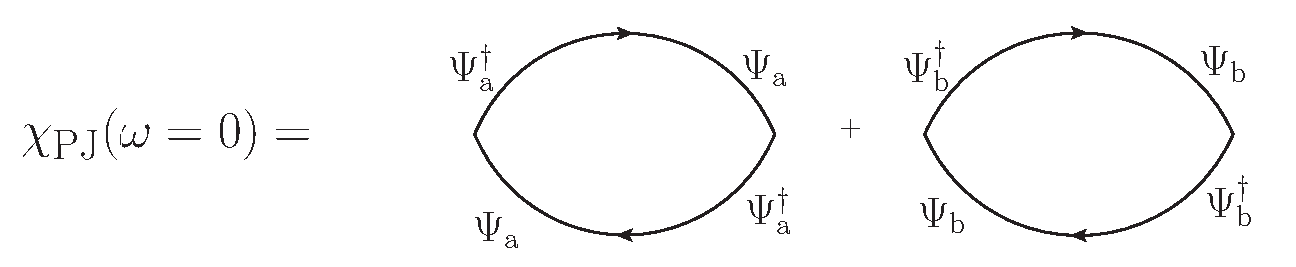
\includegraphics[width=0.8\textwidth]{static_susceptibility.eps}
	\caption{caption}
	\label{fig:static susceptibility}
\end{figure}
%
Wick's theorem is used to seperate the remaining two expectation values in terms of free Green functions.
The contraction of operators with different time argument is generated the two bubble diagrams, depicted in figure \ref{fig:static susceptibility}
The static susceptibility is given by
%
\begin{align}
	\chi_{\mt{PJ}}(\omega = 0) &= 
		\int\limits_{0}^{\beta} \dd{\tau} 
		\int_{\vb{k}} 
		k_{j}^{2}
		\bigg[
			\frac{1}{m_{1}}
			\mathcal{G}_{\mt{a}}^{(0)}(\vb{k},-\tau)
			\mathcal{G}_{\mt{a}}^{(0)}(\vb{k},\tau)
			+
			\frac{1}{m_{2}}
			\mathcal{G}_{\mt{b}}^{(0)}(\vb{k},-\tau)
			\mathcal{G}_{\mt{b}}^{(0)}(\vb{k},\tau)
		\bigg].
\end{align}
%
Here the free fermionic propagator $\mathcal{G}_{\alpha}^{(0)}(\vb{k},\tau) = -\expval*{\mathcal{T}_{\tau} \Psi_{\alpha}(\vb{k},\tau) \Psi_{\alpha}^{\dag}(\vb{k},0)}$ with $\alpha \in \{\mt{a},\mt{b}\}$ is inserted.
Both fermionic Green functions are transformed into the Matsubara frequency space.
The only $\tau$-dependence is thus given by the exponential functions.
The $\tau$-integral is evaluated, using the definition of the $\delta$-distribution in Matsubara space, $\int_{0}^{\beta} \dd{\tau} \exp(i(\omega_{m} - \omega_{n})\tau) = \beta \delta(\omega_{m} - \omega_{n})$.
One of the two sums over Matsubara frequencies is easily performed due to this $\delta$-distribution.
The obtained expression is given by
%
\begin{align}
	\chi_{\mt{PJ}}(\omega = 0) &= 
		\frac{1}{\hbar} 
		\int_{\vb{k}} 
		k_{j}^{2}
		\bigg[
			\frac{1}{m_{1}}
			S_{\mt{a}}(\omega_{n})
			+
			\frac{1}{m_{2}}
			S_{\mt{b}}(\omega_{n})
		\bigg].
\end{align}
%
The Matsubara sum $S_{\alpha}(\omega_{n}) = \beta^{-1} \sum_{\omega_{n}} \mathcal{G}_{\alpha}^{(0)}(\vb{k},\omega_{n}) \mathcal{G}_{\alpha}^{(0)}(\vb{k},\omega_{n})$, where $\alpha = \mt{a}, \mt{b}$, is defined.
This sum is transformed into a complex contour integral, offering the use of the usual complex analysis.
The product of Green functions multiplied with the Fermi distribution are generated the integrand of this contour integral.
The full transformation rule is given by
%
\begin{align}
	S = \frac{1}{\beta} \sum\limits_{\omega_{n}} \mathcal{G}(\omega_{n}) = -\frac{1}{2\pi i} \oint_{\Gamma} \dd{z} n_{\mt{F}}(z) \mathcal{G}(z).
\end{align}
%
The choice of the contour is arbitrary beside one condiction.
All singularies of the Green functions are excluded in the contour, while the infinite poles $\omega_{n} = \flatfrac{(2n+1)\pi}{\beta}$, where $n\in\mathbb{Z}$, of the Fermi distribution are included in the contour.
Our starting contour $\Gamma$ is depicted on the left hand side in figure \ref{fig:contour simple poles}.

The contour is generated by to path along the imaginary axis, from $i\infty$ to $-i\infty$ and vice versa.
Both paths are connected in plus and minus infinity and shifted infinitesimal aside the imaginary axis.
This contour is now expaned to a circle with radius infinity, where always the singularities of the Green function is excluded.
The obtained contour is depicted on the right hand side in figure \ref{fig:contour simple poles}.
The same magnitude with opposite sign is generated by the paths from infinity to the poles and vice versa.
Therefore, the contour is seperated into small circles around the poles of the Green functions and into one circle with infinite radius.
The contribution of the latter is zero, since the Green function is proportional to $\flatfrac{1}{z}$.
In the remaining contour integrals the product of Green functions is now inserted, where the single free fermionic Green function is given by
%
\begin{figure}[t]
	\centering
	\includegraphics[width=0.8\textwidth]{contour_simple_poles.pdf}
	\caption{caption}
	\label{fig:contour simple poles}
\end{figure}
%
%
\begin{align}
	\mathcal{G}_{\alpha}(\vb{k}, i\omega_{n}) = \frac{1}{i\omega_{n} - \epsilon_{\alpha}(\vb{k})}.
\end{align}
%
$\epsilon_{\alpha}(\vb{k})$, where $\alpha = \mt{a},\mt{b}$, is the fermion's dispersion and also the singularity of the Green function.
The explicite expression is denoted in equation \eqref{eq:dispersion relations}.
Besides this singularity, the Green function is holomoph in the whole complex plane.
The contour integral is evaluated using the resiuum theorem, which yields
%
\begin{align}
	\chi_{\mt{PJ}}(\omega = 0) &= 
		- \int_{\vb{k}} 
		k_{j}^{2}
		\bigg[
			\frac{1}{m_{1}}
			\dv{n_{\mt{F}}(\epsilon_{\mt{a}}(\vb{k}))}{\epsilon_{\mt{a}}(\vb{k})}
			+
			\frac{1}{m_{2}}
			\dv{n_{\mt{F}}(\epsilon_{\mt{b}}(\vb{k}))}{\epsilon_{\mt{b}}(\vb{k})}
		\bigg]
\end{align}
%
The derivatives of the distribution function with respect to the dispersion relation are generated, since the integrand has a singularity of second order at $z_{0} = \epsilon_{\alpha}(\vb{k})$.
These two obtained integrals are exactly solvable.
Therefore the inetegrals are transformed into plane polar coordinates, where the transformation rule is given by $(k_{x}, k_{y}) = (q\sqrt{2m_{1,2}}\cos(\phi), q\sqrt{2m_{2,1}}\sin(\phi))$.
Two typs of transformation are used, since the dispersion relation of the two species of fermions differs in the contained mass terms.
The only angular dependece is originated by the $k_{j}^{2}$-term.
This term yields $\cos[2](\phi)$ or $\sin[2](\phi)$ for the $x$- or $y$-direction, respectivily.
Since the limits of the $\phi$-integral are $0$ and $2\pi$, the contribution is $\pi$ in both cases.
The upper limit of the $q$-integral is set to infity, since the integrand is decreasing fast to zero for large values of $q$.
%
\begin{align}
	\chi_{\mt{PJ}}(\omega = 0) = 
		\frac{8 \beta \pi}{(2\pi)^{2}} \sqrt{m_{1} m_{2}}
		\int\limits_{0}^{\infty} \dd{q}
		q^{3} \frac{e^{\beta(q^{2} - \mu)}}{(e^{\beta(q^{2} - \mu)} + 1)^{2}}
\end{align}
%
The obtained integral is solved, substituting $x = \beta(q^{2} - \mu)$.
The first of the two obtained integrals is evaluated using integration by parts, while the derivative of the Fermi distribution with respect to $x$ is originated in the second integral.
Performing these integrals the static susceptibility of J and P is given by
%
\begin{align}
	\chi_{\mt{PJ}}(\omega = 0) = \frac{\sqrt{m_{1} m_{2}}}{\pi \beta}\ln(e^{\beta \mu} + 1)
\end{align}
%
In the case of $\mu \gg k_{\mt{B}} T$, the exponential function is large compared to 1 and neglectable.
The static susceptibility is then temperature independent in the leading order and given by
%
\begin{align}
	\chi_{\mt{PJ}}(\omega = 0) \to \frac{\mu \sqrt{m_{1} m_{2}}}{\pi} \qquad (T \to 0)
\end{align}
% %done
%
%
\chapter{Finite Conductivity because of Breaking the Translation Symmetry via Umklapp Scattering}
\label{appch:green function}
%
%
The computation of the Green function $\mathcal{G}_{\dot{\mt{P}}\dot{\mt{P}}}(\vb{k}, z)$ in \eqref{eq:static conductivity formula} is displayed in detail in the following appendix.
The Green function is given by equation \eqref{eq:Green function}.
For using the diagrammatic technique the integral is transformed into Matsubara time $\tau = it$.
The magnitude of the Jacobi determinate is $-i$ and the upper limit is changed to $\beta = T^{-1}$.
Each time derivative is further generated an imaginary unit $i$.
The Green function is represented in Matsubara time as
%
\begin{align}
	\mathcal{G}_{\dot{\mt{P}}\dot{\mt{P}}}(\vb{k}, z) = i \int\limits_{0}^{\beta} \dd{\tau} e^{z \tau} \expval{\mathcal{T}_{\tau} \dot{\mt{P}}_{j}(\tau) \dot{\mt{P}}_{j}(0)}_{\mt{H}}.
\end{align}
%
$z$ is a complex frequency and the direction of the momentum is marked by the index $j = x,y$.
The index $H$ denotes, that the expectation value is evaluated with respect to Hamiltonian $\mt{H} = \mt{H}_{\Psi} + \mt{H}_{\Phi} + mt{H}_{\Psi\Phi}$, where the interaction between fermions and spin fluctuations is considered by the last term.
In Matsubara interaction representation, the appearing time evoluation operator is expanded up the the zeroth order.
As a consequance, corrections of the Green function, caused by the fermion-spin fluctuation interaction, are neglected.
Only the two time derivatives of momentum are therefore contained in the expectation value.
This is the only origin, where the pertubation of umklapp scattering is considered.
The Green function is given by
%
\begin{align}
	\mathcal{G}_{\dot{\mt{P}}\dot{\mt{P}}}(\vb{k}, z) = i \int\limits_{0}^{\beta} \dd{\tau} e^{z \tau} \expval{\mathcal{T}_{\tau} \dot{\mt{P}}_{j}(\tau) \dot{\mt{P}}_{j}(0)}_{\mt{H}_{0}}
\end{align}
%
where the expectation value is now evaluated with respect to the free Hamiltonian $\mt{H}_{0} = \mt{H}_{\Psi} + \mt{H}_{\Phi}$.
The time derivative of momentum is designated in equation \eqref{eq:time derivative momentum finite}.
Inserting this expression, $\mathcal{G}_{\dot{\mt{P}}\dot{\mt{P}}}(\vb{k}, z)$ is given by
%
\begin{align}
	\mathcal{G}_{\dot{\mt{P}}\dot{\mt{P}}}(\vb{k}, z) &= 
		-i 
		\sum\limits_{\mu, \lambda}
		\sum\limits_{\vb{G}_{1}, \vb{G}_{2}} 
		\mt{J}_{\vb{G}_{1}} \mt{J}_{\vb{G}_{2}} 
		\int\limits_{0}^{\beta} \dd{\tau} e^{z \tau} 
		\int_{\vb{k}_{1}}\int_{\vb{k}_{2}} G_{1,j}  G_{2,j} 
		\notag \\
		&\times
		\expval{\mathcal{T}_{\tau} \Phi_{\mu}(\vb{k}_{1},\tau) \Phi_{\mu}(-\vb{k}_{1} - \vb{G}_{1},\tau) \Phi_{\lambda}(\vb{k}_{2},0) \Phi_{\lambda}(-\vb{k}_{2} - \vb{G}_{2},0)}_{\mt{H}_{0}}.
\end{align}
%
Here, the moment integrals are extended over the first Brillouin zone, while the sum over $\vb{G}_{1}$ and $\vb{G}_{2}$ runs over all reciprocal lattice vectors.
$\vb{G}_{i}$, where $i=1,2$, is the coupling parameter with respect to the reciprocal lattice vector.
The sum over $\mu$ and $\lambda$ runs over the spatial direction of the three component bosonic field, while the direction of P is indicated by $j$.

Wick's theorem is used to seperate the expectation value in terms of free propagators.
Three contraction are possible for a an expectation value, including four bosonic, real field operators.
One of them is not contributed, since the operators to equal times are contracted.
The remaining two diagrams are both bubble diagrams and topological equivalent.
The diagram is depicted in figure \ref{fig:spin wave bubble}.

Acting Wick's theorem in momentum representation, each interchange of the bosonic operators yields a $\delta$-distribution, or more presicely, the  commutator relation.
This signifies the momentum conservation at each vertex.
One momentum integral one sum over reciprocal lattice vector and the sum over $\lambda$ are therefore evaluated directly.
The remaining vectors are renamed into $\vb{k}$ and $\vb{G}$ for the momentum and reciprocal lattice vector, respectivily.
%
%\begin{figure}
%	\centering
%	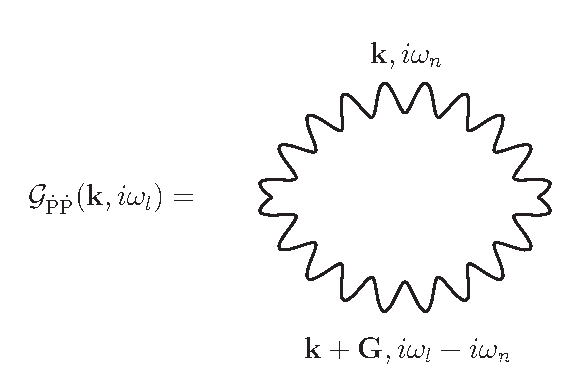
\includegraphics[width=0.5\textwidth]{spin_wave_bubble.eps}
%	\caption{}
%	\label{fig:spin wave bubble}
%\end{figure}
%
%
\begin{align}
	\mathcal{G}_{\dot{\mt{P}}\dot{\mt{P}}}(\vb{k}, z) &= 
		-2 
		\sum\limits_{\vb{G}} 
		\vert \mt{J}_{\vb{G}} \vert^{2}
		\int\limits_{0}^{\beta} \dd{\tau} e^{z \tau} 
		\int_{\vb{k}} G_{j}^{2}
		\notag \\
		&\times
		\expval{\mathcal{T}_{\tau} \Phi_{\mu}(\vb{k},\tau) \Phi_{\mu}(-\vb{k},0)}_{\mt{H}_{0}} 
		\expval{\mathcal{T}_{\tau} \Phi_{\mu}(-\vb{k} - \vb{G},\tau) \Phi_{\mu}(\vb{k}+\vb{G},0)}_{\mt{H}_{0}},
\end{align}
%
The factor of 2 is originated by the sum over both identical diagrams.
Furthermore, the relation $\mt{J}_{-\vb{G}} = \mt{J}_{\vb{G}}^{*}$ is used, where the complex conjugated is denoted by the asterisk.
The obtained expectation values are the free spin density propagtors $\mathcal{D}_{\mu}^{(0)}(\vb{k},\tau)$.
Both propagators are transformed into Matsubara frequency space, using the transformation rule
%
\begin{align}
	\mathcal{D}_{\mu}^{(0)}(\vb{k},\tau) = \frac{1}{\beta} \sum\limits_{\omega_{n}} e^{-i\omega_{n}\tau} \mathcal{D}_{\mu}^{(0)}(\vb{k},i\omega_{n})
\end{align}
%
where the summation runs over all bosonic Matsubara frequencies $\omega_{n} = \flatfrac{2n\pi}{\beta}$, where $n\in\mathbb{Z}$.
The frequency argument of the Green function is set to $z = i\omega_{l}$, since the Green function is now investigated onto the imaginary frequency axis.
The exponential functions are generated the only $\tau$-dependence and the $\tau$-integral is evaluated to $\beta \delta_{\omega_{m}+\omega_{l}-\omega_{n}}$.
One of the two sums over Matsubara frequencies is evaluated as well.
The following expression is obtained:
%
\begin{align}
	\mathcal{G}_{\dot{\mt{P}}\dot{\mt{P}}}(\vb{k}, i\omega_{l}) &= 
		-2 
		\sum\limits_{\vb{G}} 
		\vert \mt{J}_{\vb{G}} \vert^{2}
		\int_{\vb{k}} G_{j}^{2}
		\frac{1}{\beta} \sum\limits_{\omega_{n}}
		\mathcal{D}_{\mu}(\vb{k},i\omega_{n}) \,
		\mathcal{D}_{\mu}(-\vb{k}-\vb{G},i\omega_{l}-i\omega_{n}).
		\label{appeq:Green function on the imaginary axis}
\end{align}
%
In the following the Matsubara sum is evaluated.
Therefore, the singularities of both propgators are observed.
A discontinuity of the propagator, denoted in \eqref{eq:damped spin propagator}, is generated if the term of Matsubara frequancies in the denominator becomes to be zero.
%
\begin{figure}[t]
	\centering
	\includegraphics[width=\textwidth]{contour_branch_cut.pdf}
	\caption{
This figure shows the starting contour of the complex integral appearing at the computation of the Green function $\mathcal{G}_{\dot{\mt{P}}\dot{\mt{P}}}$.
The contour is seperated into three parts due to the two discontinuities at $0$ and $\omega_{l}$ (red crosses) of the Green function, reflected as branch cuts in the complex plane.
This is depicted on the left hand side.
All three contours are expanded to infinity, depicted on the right hand side.
The semicircles and the paths between both branches yield no contributions.
The remaining paths are four ones, along each side of two branches.
	}
	\label{fig:contour branch cut}
\end{figure}
%
This type of singularity is called branch cut, since the whole horizontal line along the singularity is forbidden.
In the investigated case, two singularity of them arise, where one is sited at $\omega_{n} = 0$ and the other one is sited at $\omega_{n} = \omega_{l}$.
To transform the Matsubara sum into a complex contour integral, both singularities are seperated from the sum.
For reasons of clarity the momentum argument of the second propagator is abbreviatied by $\vb{k}'=-\vb{k}-\vb{K}$ and the momentum arguments are written as a lower index.
%
\begin{align}
	S(i\omega_{l}) :&= \frac{1}{\beta} \sum\limits_{\omega_{n}} \mathcal{D}_{\mu,\vb{k}}(i\omega_{n}) \, \mathcal{D}_{\mu,\vb{k}'}(i\omega_{l}-i\omega_{n})
	\notag \\
	\Leftrightarrow\ S(i\omega_{l}) :&= 
		\frac{1}{\beta} \mathcal{D}_{\mu,\vb{k}}(0) \, \mathcal{D}_{\mu,\vb{k}'}(i\omega_{l})
		+
		\frac{1}{\beta} \mathcal{D}_{\mu,\vb{k}}(i\omega_{l}) \, \mathcal{D}_{\mu,\vb{k}'}(0)
		\notag \\
		&+
		\frac{1}{\beta} \sum\limits_{\substack{n \neq 0 \\ n \neq l}} \mathcal{D}_{\mu,\vb{k}}(i\omega_{n}) \, \mathcal{D}_{\mu,\vb{k}'}(i\omega_{l}-i\omega_{n})
	\label{appeq:seperated Matsubara sum}
\end{align}
%
The remaining sum, labeled with $\mt{I}_{MS}(\omega_{l})$ in the following, is now transformed into a complex contour integral.
All Matsubara frequencies are included into the contour $\Gamma$, beside the two seperated frequencies.
Similar to the case of simple poles, see \ref{appch:static susceptibility}, the contour runs along the imaginary axis.
The contour is closed infinitesimal above and below the banches, since crossing of the branches is forbidden.
The contour $\Gamma$ is depicted on the left hand side in figure \ref{fig:contour branch cut}.
Since the spin propagators are bosonic, the Bose distribution $n_{\mt{B}}(z)$ is considered, transforming the sum into a contour integral.
%
\begin{align}
	\mt{I}_{MS}(\omega_{l}) := 
		\frac{1}{\beta} \sum\limits_{\substack{n \neq 0 \\ n \neq l}} \mathcal{D}_{\mu,\vb{k}}(i\omega_{n}) \, \mathcal{D}_{\mu,\vb{k}'}(i\omega_{l}-i\omega_{n})
		=
		\oint\limits_{\Gamma} \frac{\dd{z}}{2\pi i} n_{\mt{B}}(z) \mathcal{D}_{\mu,\vb{k}}(z) \, \mathcal{D}_{\mu,\vb{k}'}(i\omega_{l}-z)
\end{align}
%
As shown in figure \ref{fig:contour branch cut} $\Gamma$ is seperated in three single contours, denoted as $\Gamma_{1}$, $\Gamma_{2}$ and $\Gamma_{3}$.
These three contours are expanded to infity where the contour path is never allowed to cross the horizontal line at $\omega_{l}$ or $0$.
The obtained contour is depicted on the right hand side in figure \ref{fig:contour branch cut}.

The contour $\Gamma_{1}$ is taken along the real axis in negative direction and is closed by a semi-circle with infinite radius in the lower complex plane.
$\Gamma_{2}$ is the contour between both branch cuts.
The contour is started along the real axis in positive direction.
At infinity the contour is perfomed up to the branch at $\omega_{n}$.
The path is taken in oppsite direction to minus infinity and from there dwon to the starting point.
The last contour $\Gamma_{3}$ is taken along the $\omega_{n}$-axis in positive direction and is closed by a semi-circle with infinite radius in the upper complex plane.
The contours parallel the real and $\omega_{n}$-axis is set infinitesimal beside these axis, which is indicated with the term $\pm i\eta$.
The sign is chosen according to the corresponding contour.

Each one of these three contour integrals can be splitted in parts, where only the parts parallel to the real axis do not vanish.
In all other segments the path is lying in infinity and, since the integrand is decreasing faster than $\flatfrac{1}{z}$ for $z \to \infty$, these part are zero.
Only, the paths survive along the two branch cuts.
%
\begin{align}
	\mt{I}_{MS}(\omega_{l}) &= 
		\int\limits_{-\infty}^{\infty} \frac{\dd{\epsilon}}{2\pi i} 
			\mathcal{D}_{\mu,\vb{k}'}(i\omega_{l}-\epsilon)
			\bigg[
				n_{\mt{B}}(\epsilon - i\eta) 
				\mathcal{D}_{\mu,\vb{k}}(\epsilon - i\eta) 
				- 
				n_{\mt{B}}(\epsilon + i\eta) 
				\mathcal{D}_{\mu,\vb{k}}(\epsilon + i\eta)
			\bigg]
		\notag \\ &+
		\int\limits_{-\infty}^{\infty} \frac{\dd{\epsilon}}{2\pi i} 
			\mathcal{D}_{\mu,\vb{k}}(i\omega_{l} + \epsilon)
			\bigg[
				n_{\mt{B}}(i\omega_{l} + \epsilon - i\eta)  
				\mathcal{D}_{\mu,\vb{k}'}(\epsilon - i\eta) 
				\notag \\& \hspace{3.6cm}- 
				n_{\mt{B}}(i\omega_{l} + \epsilon + i\eta)
				\mathcal{D}_{\mu,\vb{k}'}(\epsilon + i\eta)
			\bigg]
	\label{appeq:Matsubara sum along axes parallel to real axis}
\end{align}
%
The limit $\eta \to 0^{+}$ is implied and the symmetry property with respect to the frequency is used.
Now, the Bose distribution is simplified.
Firstly the relation $n_{\mt{B}}(z+i\omega_{l}) = n_{\mt{B}}(z)$ is used, which follows directly from the definition of the bosonic Matsubara frequencies $\omega_{n} = \flatfrac{2n\pi}{\beta}$, where $n\in\mathbb{Z}$.
Inserting them into the Bose distribution, the exponential function is always evaluated to 1, since $\exp(i2\pi) = 1$.
The Bose distribution is transformed onto the real axis using analytical continuation.
The complex frequency $z$ is expressed as $\epsilon \pm i\eta$, where the limit $\eta \to 0^+$ is implied.
The exponential function in $n_{\mt{B}}(\epsilon \pm i\eta)$ is expanded up the second order, since the first order is chanceled.
%
\begin{align}
	n_{\mt{B}}(\epsilon \pm i\eta) \approx \frac{\beta^{-1}}{\epsilon \pm i\eta} = \beta^{-1} \Big( \PV{\frac{1}{\epsilon}} \mp i\pi\delta(\epsilon) \Big) \approx n_{\mt{B}}(\epsilon) \mp i\pi \beta^{-1} \delta(\epsilon),
	\label{appeq:Bose distribution in real and imaginary part}
\end{align}
%
The last equality is only valid for small frequencies.
In equation \eqref{appeq:Matsubara sum along axes parallel to real axis}, the Matsubara frequencies are eliminated in the argument of both Bose distributions.
Both squared brackets under the integral are quite identical, beside the different momentum argument of the propagator.
Our next approach is writing the Bose distribution  and the propagators into real and imaginary parts.
The real part of them are symmetric and the imaginary part of them is antisymmetric with respect to change $\eta$ to $-\eta$.
The following expression is obtained for the squared brackets in the first line of \eqref{appeq:Matsubara sum along axes parallel to real axis}:
%
\begin{align}
	2i\Big[ \Re{n_{\mt{B}}(\epsilon+i\eta)} \Im{\mathcal{D}_{\mu, \vb{k}}(\epsilon+i\eta)} + \Im{n_{\mt{B}}(\epsilon+i\eta)} \Re{\mathcal{D}_{\mu, \vb{k}}(\epsilon+i\eta)} \Big].
	\label{appeq:conversion of squared brackets}
\end{align}
%
An analogical expression is obtained for the squared brackets in the second line changing $\vb{k}$ to $\vb{k}'$ and vice versa.
The second term of \eqref{appeq:conversion of squared brackets} is evaluated first.
The imaginary part of the Bose distribution is given by equation \eqref{appeq:Bose distribution in real and imaginary part}.
The equivalent procedure is performed for the second bracket in \eqref{appeq:Matsubara sum along axes parallel to real axis}.
Both relations are integrated with respect to $\epsilon$.
Using relation $\Re{\mathcal{D}_{\mu,\vb{k}}(0)} = \mathcal{D}_{\mu,\vb{k}}(0)$, the obtained expression is equivalent to the seperated terms in equation \eqref{appeq:seperated Matsubara sum}, beside a minus sign.
%
\begin{align}
	-\frac{1}{\beta} \mathcal{D}_{\mu,\vb{k}'}(i\omega_{l}) \mathcal{D}_{\mu,\vb{k}}(0) - \frac{1}{\beta} \mathcal{D}_{\mu,,\vb{k}}(i\omega_{l}) \mathcal{D}_{\mu,\vb{k}'}(0)
\end{align}
%
These both therms are chanceled the seperated terms in \eqref{appeq:seperated Matsubara sum}
The remaining contributions of $S(i\omega_{l})$ are given by the first term of equation \eqref{appeq:conversion of squared brackets} and the corresponding term for the second squared brackets in \eqref{appeq:Matsubara sum along axes parallel to real axis}.
The real part of the Bose distribution $n_{\mt{B}}(\epsilon + i\eta)$ is the Bose distribution itself (see \eqref{appeq:Bose distribution in real and imaginary part})
Since the imaginary part of $\mathcal{D}_{\mu}$ is independent of the additional part $i\eta$ the Matsubara sum is given by
%
\begin{align}
	S(i\omega_{l}) = \int\limits_{-\infty}^{\infty} \frac{\dd{\epsilon}}{\pi} 
			n_{\mt{B}}(\epsilon) 
			\bigg[
				\mathcal{D}_{\mu,\vb{k}'}(i\omega_{l} - \epsilon) \Im{\mathcal{D}_{\mu, \vb{k}}(\epsilon)}
				+ 
				\mathcal{D}_{\mu,\vb{k}}(i\omega_{l} + \epsilon) \Im{\mathcal{D}_{\mu, \vb{k}'}(\epsilon)}
			\bigg]
\end{align}
%
$S(i\omega_{l})$ is now transformed on the real axis, using analytical continuation, $i\omega_{l} = \omega + i\eta =: \tilde{\omega}$.
The Matsubara sum is given by
%
\begin{align}
	S(\omega) = \int\limits_{-\infty}^{\infty} \frac{\dd{\epsilon}}{\pi} 
			n_{\mt{B}}(\epsilon) 
			\bigg[
				\mathcal{D}_{\mu,\vb{k}'}^{*}(\epsilon - \omega) \Im{\mathcal{D}_{\mu, \vb{k}}(\epsilon)}
				+ 
				\mathcal{D}_{\mu,\vb{k}}(\epsilon + \omega) \Im{\mathcal{D}_{\mu, \vb{k}'}(\epsilon)}
			\bigg]
\end{align}
%
Here, relation $\mathcal{D}_{\mu,\vb{k}'}(\omega - \epsilon) = \mathcal{D}_{\mu,\vb{k}'}^{*}(\epsilon - \omega)$ is used, following from equation \eqref{appeq:damped spin density propagator with real omega}.
The frequency argument is shifted from $\epsilon - \omega$ to $\epsilon$ in the first term.
The imaginary part of the retarded Green function is used in the calculation of the conductivity or resistance.
Considering equation \eqref{appeq:Green function on the imaginary axis}, the Matsubara sum is the only observed complex quantity.
The imaginary part of the Matsubara sum is given by
%
\begin{align}
	\Im{S(\omega)} = 
		\int\limits_{-\infty}^{\infty} \frac{\dd{\epsilon}}{\pi} 
		\bigg[ n_{\mt{B}}(\epsilon) - n_{\mt{B}}(\epsilon + \omega)\bigg] 
		\Im{\mathcal{D}_{\mu}(-\vb{k}-\vb{G},\epsilon)} 
		\Im{\mathcal{D}_{\mu}(\vb{k}, \epsilon + \omega)}
\end{align}
%
where $\Im{\mathcal{D}^{*}} = - \Im{\mathcal{D}}$ is used.
The imaginary part of the retarded Green function is obtained by inserting the expression for $\Im{S(\omega)}$.
%
\begin{align}
	\Im{\mathcal{G}_{\dot{\mt{P}}\dot{\mt{P}}}^{\mt{ret}}(\omega)} &= 
		-2 
		\sum\limits_{\vb{G}} 
		\vert \mt{J}_{\vb{G}} \vert^{2}
		\int\limits_{-\infty}^{\infty} \frac{\dd{\epsilon}}{\pi} 
		\bigg[n_{\mt{B}}(\epsilon) - n_{\mt{B}}(\epsilon + \omega)\bigg]
		\notag \\
		&\times
		\int_{\vb{k}} G_{j}^{2}
		\Im{\mathcal{D}_{\mu}(-\vb{k}-\vb{G},\epsilon)} 
		\Im{\mathcal{D}_{\mu}(\vb{k}, \epsilon + \omega)},
\end{align}
%
The imaginary part of the spin propagator is denoted in equation \eqref{appeq:real and imaginary part of D}.
Small frequencies $\omega$ are considered, since our interest is based on the static electrical conductivity.
Spin propagators and Bose distributions are investigated seperately in this limit.
The latter is expanded up to the first order, since the zeroth order vanishes.
In the case of spin propagators, $\omega$ is simply set to zero.
The first derivative of the Bose distribution and both spin propagators are even function with respect to $\epsilon$.
Therefore, the lower boundary of the integral is set to zero and the integral is multiplied by 2.
Inserting the explicite expressions for the imaginary parts of the propagators, the imaginary part of the retarded Green function is obtained.
%
\begin{align}
	\Im{\mathcal{G}_{\dot{\mt{P}}\dot{\mt{P}}}^{\mt{ret}}(\omega)} &= 
		-\frac{4 \gamma^{2} \beta \omega}{\pi}
		\sum\limits_{\vb{Q}_{1}, \vb{Q}_{2}}
		\sum\limits_{\vb{G}}
		\vert \mt{J}_{\vb{G}} \vert^{2}
		\int\limits_{0}^{\infty} \dd{\epsilon}
		\frac{\epsilon^{2} e^{\beta \epsilon}}{(e^{\beta \epsilon} - 1)^{2}}
		\notag \\
		&\times
		\int_{\vb{k}} G_{j}^{2} \cdot
		\frac{1}{(\vb{k}+\vb{G}-\vb{Q}_{1})^{4} + \gamma^{2} \epsilon^{2}} \cdot
		\frac{1}{(\vb{k} + \vb{Q}_{2})^{4} + \gamma^{2} \epsilon^{2}}
		\label{appeq:imaginary part Green function on the real axis}
\end{align}
%


























 %done
%
%
\chapter{Properties of the Kubo Relaxation Function}
\label{app:properties of the Kubo relaxation function}
%
%
In section \ref{sec:kubo relaxation function} the Kubo relaxation function 
%
\begin{align}
	\Phi_{\mt{AB}}(t) = \frac{i}{\hbar} \lim\limits_{s \to 0} \int\limits_{t}^{\infty} \dd{\tau} \expval{\comm{\mt{A}_{\mt{I}}(\tau)}{\mt{B}_{\mt{I}}(0)}}_{0} e^{-s\tau}.
	\label{appeq:Kubo relaxation function}
\end{align}
%
and the three relations 
%
\begin{enumerate}
	\item $\begin{aligned}[t] \chi_{\mt{AB}}(t) = -\Theta(t) \dv{t} \Phi_{\mt{AB}}(t) \end{aligned}$\hfill \refstepcounter{equation}(\theequation)\label{appeq:relation 1 between Phi and chi}
	\item $\begin{aligned}[t] \Phi_{\mt{AB}}(t = 0) = \chi_{\mt{AB}}(\omega = 0) \end{aligned}$\hfill \refstepcounter{equation}(\theequation)\label{appeq:relation 2 between Phi and chi}
	\item $\begin{aligned}[t] \Phi_{\mt{AB}}(\omega) = \frac{1}{i\omega}\big[\chi_{\mt{AB}}(\omega) - \chi_{\mt{AB}}(\omega = 0)\big]. \end{aligned}$\hfill \refstepcounter{equation}(\theequation)\label{appeq:relation 3 between Phi and chi}
\end{enumerate}
%
connecting the dynamical susceptibility $\chi_{\mt{AB}}$ with $\Phi_{\mt{AB}}$ are introduced.
In the following we want to proof these three relations.

The first one is easly gotten by derivating the Kubo relaxation function with respect to $t$ and comparing the result with the definition of the dynamical susceptibility \eqref{eq:dynamical susceptibilty}.
%
\begin{align}
	-\Theta(t) \dv{t} \Phi_{\mt{AB}}(t) = \frac{i}{\hbar} \Theta(t) \expval{\comm{\mt{A}_{\mt{I}}(t)}{\mt{B}_{\mt{I}}(0)}}_{0} = \chi_{\mt{AB}}(t)
\end{align}
%
The second relation is found with the aim of the Laplace transformation of the Kubo relaxation function.
%
\begin{align}
	\Phi_{\mt{AB}}(\omega) = \int\limits_{0}^{\infty} \dd{t} \Phi_{\mt{AB}}(t) e^{i\omega t}
	\label{appeq:Laplace transformation imaginary axis}
\end{align}
%
In this definition of the Laplace transformation we set $s = -i\omega$ which correspond to a rotation of $\frac{\pi}{2}$ of the definition space.
Using \eqref{appeq:Laplace transformation imaginary axis} after setting $t = 0$ in \eqref{appeq:Kubo relaxation function} yield
%
\begin{align}
	\Phi_{\mt{AB}}(t=0) &= \frac{i}{\hbar} \lim\limits_{s \to 0} \int\limits_{0}^{\infty} \dd{\tau} \expval{\comm{\mt{A}_{\mt{I}}(\tau)}{\mt{B}_{\mt{I}}(0)}}_{0} e^{-s\tau}
	\notag \\
	\Leftrightarrow\ \Phi_{\mt{AB}}(t=0) &= \frac{i}{\hbar} \lim\limits_{\substack{s \to 0 \\ \omega \to 0}}\ \int\limits_{-\infty}^{\infty} \dd{\tau} \Theta(\tau) \expval{\comm{\mt{A}_{\mt{I}}(\tau)}{\mt{B}_{\mt{I}}(0)}}_{0} e^{i\omega \tau} e^{-s\tau}
	\notag \\
	\Leftrightarrow\ \Phi_{\mt{AB}}(t=0) &= \lim\limits_{\omega \to 0}\ \int\limits_{-\infty}^{\infty} \dd{\tau} \chi_{\mt{AB}}(\tau) e^{i\omega \tau}
	\notag \\
	\Leftrightarrow\ \Phi_{\mt{AB}}(t=0) &= \chi_{\mt{AB}}(\omega = 0),
\end{align}
%
where it is assumed the susceptibility is a good function in the sense they decay fast enough and the convergence generating faktor is negligible.
The third relation is computated with the aim of the first and second relation.
Therefore relation one is multiplied with $e^{i\omega t}$ and is integrated with respect to $t$.
%
\begin{align}
	\int\limits_{0}^{\infty} \dd{t} e^{i\omega t} \chi_{\mt{AB}}(t)  &= - \int\limits_{0}^{\infty} \dd{t} e^{i\omega t} \dv{t} \Phi_{\mt{AB}}(t)
	\notag \\
	\overset{\mt{PI}}{\Leftrightarrow}\ \chi_{\mt{AB}}(\omega) &= \eval{-e^{i\omega t} \Phi_{\mt{AB}}(t)}_{0}^{\infty} + i\omega \int\limits_{0}^{\infty} \dd{t} e^{i\omega t} \Phi_{\mt{AB}}(t)
	\notag \\
	\Leftrightarrow\ \chi_{\mt{AB}}(\omega) &= \Phi_{\mt{AB}}(t=0) + i\omega \Phi_{\mt{AB}}(\omega)
	\notag \\
	\Leftrightarrow\ \Phi_{\mt{AB}}(\omega) &= \frac{1}{i\omega} \big[\chi_{\mt{AB}}(\omega) - \chi_{\mt{AB}}(\omega=0)\big]
\end{align}
%
In the first step the right hand side is integrated by parts and in last step the first relation and \eqref{appeq:Laplace transformation imaginary axis} is used.
So the third relation gives us the dependence between the Kubo relaxation function and the dynamical susceptibility in frequency space. 
%\input{chapters/appendix_fierz_identity}

\endgroup
%
\backmatter
%
\cleardoublepage
\listoftodos
%
\cleardoublepage
%\printbibliography
%
\end{document}